\chapter{Top Squark Production and Backgrounds}
\label{ch:Search}

We have now motivated that the top squark, \st{}, could be the lightest squark, see Sec. \ref{subsec:StopMassSpec}. This allows us to possibly produce this squark at CMS. In Sec. \ref{sec:Baseline}, we have designed a search that will look for event with large amounts of \met{} and \nj. These events are being targeted in separate low \dm{} and high \dm{} search regions. For all of these we are interested in the expected amount of signal and background in each region. We will look at the production and decay modes of various \st{} interactions and look into the estimation of the SM background of each region. 

\section{Production and Decay Modes}
\label{sec:Production}

Now we will look at at the production modes and backgrounds of the \st{} squark decay. To produce the top squark all we need is the collision of two proton-proton beams. It is shown as a black circle in the Fig. \ref{fig:stop-gluino-production} and \ref{fig:stop-direct-production}. This is meant to represent many processes that can make a top squark. The main processes are gluon fusion, when two gluons fuse into a single gluon which then decays into a top and anti-top squark pair, or annihilation, where two quarks annihilate to a gluon propagator which thus decays into two top squarks. 

\begin{figure}[!h]
	\begin{center}
		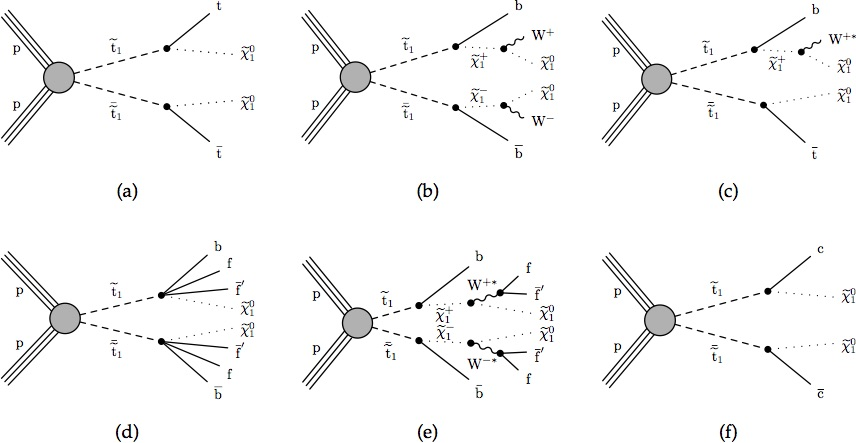
\includegraphics[width=1.00\textwidth]{T2tt_all.jpg}
	\end{center}
	\caption[Direct stop production]{Feynman diagrams for the direct \st{} production in SUSY. The allowed decay modes are (a) T2tt, (b) T2bW, (c) T2tb, (d,e) T2fbd, and (f) T2cc. }
	\label{fig:stop-direct-production}
\end{figure}

\begin{figure}[!h]
	\begin{center}
		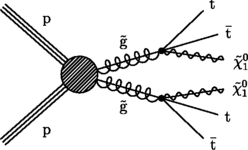
\includegraphics[width=0.32\textwidth]{T1tttt.png}
		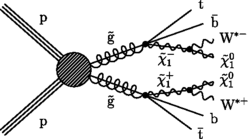
\includegraphics[width=0.32\textwidth]{T1ttbb.png} \\
		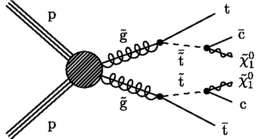
\includegraphics[width=0.32\textwidth]{T5ttcc.png}
		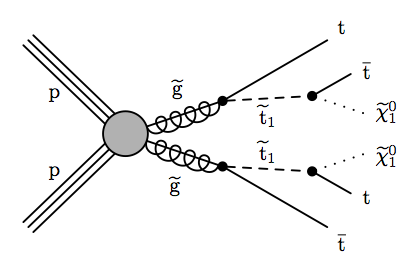
\includegraphics[width=0.32\textwidth]{T5tttt.png} \\
	\end{center}
	\caption[Gluino mediated stop production]{Feynman diagrams for the indirect \st{} production in SUSY. The allowed decay modes are T1tttt (top left), T1ttbb (top right), T5ttcc (bottom left), and T5tttt (bottom right).
	}
	\label{fig:stop-gluino-production}
\end{figure}


The main decay mode of the top squark is $\st\rightarrow t+\neutralino$ and $\st\rightarrow b+\chargino$, Fig. \ref{fig:stop-direct-production}. The top quark most likely decays as. $t\rightarrow b\W$, while the $b$ quark will decay to either a $c$ or an $u$ quark in its decay chain with an additional \W{} boson. The \neutralino{} is proposed to be a stable dark matter candidate while the \chargino could decay as, $\chargino\rightarrow\neutralino\W$. Next, a four body decay is allowed for, $\st\rightarrow b f f^\prime \neutralino$, see Fig. \ref{fig:stop-direct-production}.

\section{Standard Model Background}
\label{sec:SMBackground}

The standard model background for the top squark search is defined by a large \met{} and a multiple jets. The are a couple types of SM background that can be misinterpretted as our signal. The most likely background is that which causes many tops (or heavy particles) and missing energy. Events in the SM like \ttbar{} and \W+jets will have many jets projuced and \met{} due to missing the lepton produced. The production of heavy particles like \Znunu{} will give mutliple jets and \met{} from the neutrinos being missed by the detector. QCD events often produce events with multiple jets, due to acceptances in the detector the jets can sometimes be mis-measured which can cause large \met{}. There are also various processes that are quite rare which are quite rare but still need to be accounted for. 

\section{Lost Lepton}
\label{subsec:LL}

The contribution from the \ttbar{} and \W+jets processes arises from leptonic decays of the \W{} boson where the charged lepton is outside the kinematic acceptance of CMS or evades identificaiton by the dedicated lepton vetoes. Large \met{} can be generated by the associated neutrino and the lepton that is not reconstructed, allowing such events to enter the search regions. This background is collectively referred to as the "Lost Lepton" (LL) background. Contributions arising from $ttW$ and single-top processes also enter into this category, but with much smaller importance. 

Studies in simulation indicate that the event kinematics for different lepton flavors are similar enough to allow us to estimate them collectively from a single control sample in data that has event characteristics similar to those of the search sample. Because of this, we use the single-lepton control sample to estimate the LL background, using the method descrived in detail in Ref. [18]. The single-lepton sample consists of events that have one lepton satisfying the lepton-veto criteria. In order to suppress potential signal contamination, we require $M_T(l,\met)<100~\GeV$. If there is more than one selected lepton, we randomly select which lepton is chosen to determine the $M_T(l,\met)$. The requirement of low $M_T(l,\met)$ also ensures orthogonality to the search regions used in the search for direct top squark production in the single-lepton final state, making it possible to statistically combine the results of the two searches. The selection applied to the single-lepton control sample follows the same selection on the search variables as in the zero-lepton selection with the exception of classification according to the number of top and \W-tagged candidates. 

\subsection{Combining All Run 2 Eras}\label{sec:LLCombination}
Firstly, for this analysis we are interested in the possibility in combining the yields of each era into one estimation. This is initially done by looking at the \met{} distributions in each era, see Fig. \ref{fig:llb-1lcr-datavsmc-lm-inclusive} and \ref{fig:llb-1lcr-datavsmc-hm-inclusive}. These all have a good agreement between Data and MC. 
\begin{figure}[!htb]
	\begin{center}
  \includegraphics[width=0.32\textwidth]{../Research/SUSY/2019/LLB/njets20_v3/MET_pt_DataMC___llcr_lm_RunBtoE_2017_allPU.pdf}
  \includegraphics[width=0.32\textwidth]{../Research/SUSY/2019/LLB/njets20_v3/MET_pt_DataMC___llcr_lm_RunF_2017_allPU.pdf} \\
  \includegraphics[width=0.32\textwidth]{../Research/SUSY/2019/LLB/njets20_v3/MET_pt_DataMC___llcr_lm_PreHEM_2018_allPU.pdf}
  \includegraphics[width=0.32\textwidth]{../Research/SUSY/2019/LLB/njets20_v3/MET_pt_DataMC___llcr_lm_PostHEM_2018_allPU.pdf} \\
	\end{center}
	\caption{Comparison of the Data and MC in the 1Lep CR for each era: Run2016, Run2017BtoE, Run2017F, Run2018preHEM, Run2018PostHEM, and the combination of all eras in the Low \dm{} region. Each era has a good agreement between Data and MC. 
	 }
	\label{fig:llb-1lcr-datavsmc-lm-inclusive}
\end{figure}
\begin{figure}[!htb]
	\begin{center}  
		\includegraphics[width=0.32\textwidth]{../Research/SUSY/2019/LLB/njets20_v3/MET_pt_DataMC___llcr_hm_RunBtoE_2017_allPU.pdf}
		\includegraphics[width=0.32\textwidth]{../Research/SUSY/2019/LLB/njets20_v3/MET_pt_DataMC___llcr_hm_RunF_2017_allPU.pdf} \\
		\includegraphics[width=0.32\textwidth]{../Research/SUSY/2019/LLB/njets20_v3/MET_pt_DataMC___llcr_hm_PreHEM_2018_allPU.pdf}
		\includegraphics[width=0.32\textwidth]{../Research/SUSY/2019/LLB/njets20_v3/MET_pt_DataMC___llcr_hm_PostHEM_2018_allPU.pdf}
	\end{center}
	\caption{Comparison of the Data and MC in the 1Lep CR for each era: Run2016, Run2017BtoE, Run2017F, Run2018preHEM, Run2018PostHEM, and the combination of all eras in the High \dm{} region. Each era has a good agreement between Data and MC. 
	 }
	\label{fig:llb-1lcr-datavsmc-hm-inclusive}
\end{figure}


\subsubsection{Transfer Factors}
\label{subsec:TF}

The LL estimation in each search region is based upon the event count in data in the corresponding control region in the single-lepton sample. The count is extrapolated to the search region to obtain a prediction by means of a transfer factor obtained from simulation samples as follows: 

\begin{equation}
\label{eqn:LLTF}
N_{pred}^{LL}=TF_{LL} \cdot N_{data}(1l).
\end{equation}

We want to suppress signal contamination by requiring $M_{T}(l, \met) < 100$ GeV. This requirement confirms that it is orthogonal to the search reagions that are used in the search for direct top squark production in the single-lepton final state. Letting the two anaysis statistically combine the results in the future. 

This allows us to have the same selection for the single-lepton control sample and the zero-lepton sample. The only exception is the number of top and W-tagged candidates? what is the difference betweeen a candidate and a particle?

The LL estimation is dependent on the yield of data in the corresponding CR and the TF calculated by the single-lepton sample. The transfer factor is defined as, 
\begin{equation}
\label{eqn:TF}
TF_{LL}=\frac{N_{MC}(0l)}{N_{MC}(1l)},
\end{equation}
where $N_{MC}(1l)$ is the event count observed in the corresponding CR and $N_{MC}(0l)$ use the event count in the corresponding SR. 

The main motivation behind this approach is to increase the statistical precision of the background estimation. The performance of the $t$ and \W{} taggers is studied in data and MC samples. Reasonably good agreement is observed allowing us to procedd with this approach. Data-to-MC scale factors are extracted and applied to MC to account for residual differences of the tagging performance in data. Detailed studies comparing the performance of the $t$ and \W{} taggers in data and MC are documented in App. BLANK and BLANK.

The control regions utilized to predict the LL background are displayed in Fig. \ref{fig:llb-1lcr-datavsmc-lm-nb0} to \ref{fig:llb-1lcr-datavsmc-hm-nb3-2}. The figures \ref{fig:llb-1lcr-datavsmc-lm-nb0} to \ref{fig:llb-1lcr-datavsmc-lm-nb1} display the control regions specific to the low \dm{} selection, where the regions are binned following the search region definition. Figures \ref{fig:llb-1lcr-datavsmc-hm-nt0-nrt0-nw0} to \ref{fig:llb-1lcr-datavsmc-hm-nb3-2} display the control regions dedicated for the high \dm{} selection. Due to the nature of the background estimation method applied in the high \dm{} search, control regions are utilized for the prediction of multiple search regions. 

Tables \ref{tab:0l-llb-pred-lm} to \ref{tab:0l-llb-pred-hm-3} summarize the yields in data observed in the single-lepton sample, the derived transfer factor, and the resulting LL predictions for the low \dm{} and high \dm{} search regions respectively. The transfer factors in the high \dm{} region actually account for two levels of extrapolation, i.e., the extrapolation from the control regions to the search regions without the requirement of $t$ and \W{} tags, and extrapolation in top and \W{} tags in the search regions after correcting the top- and W-tagging efficiencies:
\begin{equation}\label{TFExtrapolation}
\begin{split}
TF_{LL}=& TF_{LL}^{CR-SR}\times TF_{LL}^{SR-extrap} \\
=& \frac{N_{MC}(0l)(\nj,\nb,\met)}{N_{MC}(1l)(\nj,\nb,\met)}\times\frac{N_{MC}(0l)(\nj,\nb,\met,\nt,\nrt,\nw)}{N_{MC}(0l)(\nj,\nb,\met)}.
\end{split}
\end{equation}

We now want to consider how the transfer factor for each era relates to the total transfer factor. In Fig. \ref{fig:llb-1lcr-datavsmc-total-tf} and \ref{fig:llb-1lcr-datavsmc-sep-tf}, we see the comparison the the total $TF$ for each era of the data and simulation. these are all in quite good agreement, but we see are large peak near zero. Once we alter the comparison for the $TF$ for the CR-to-SR and the SR-to-Extrapolation. We see a much better agreement when we do not include the cuts on top/W tagging. These are improved because of the better statistics in the region. 
\begin{figure}
	\begin{center}
  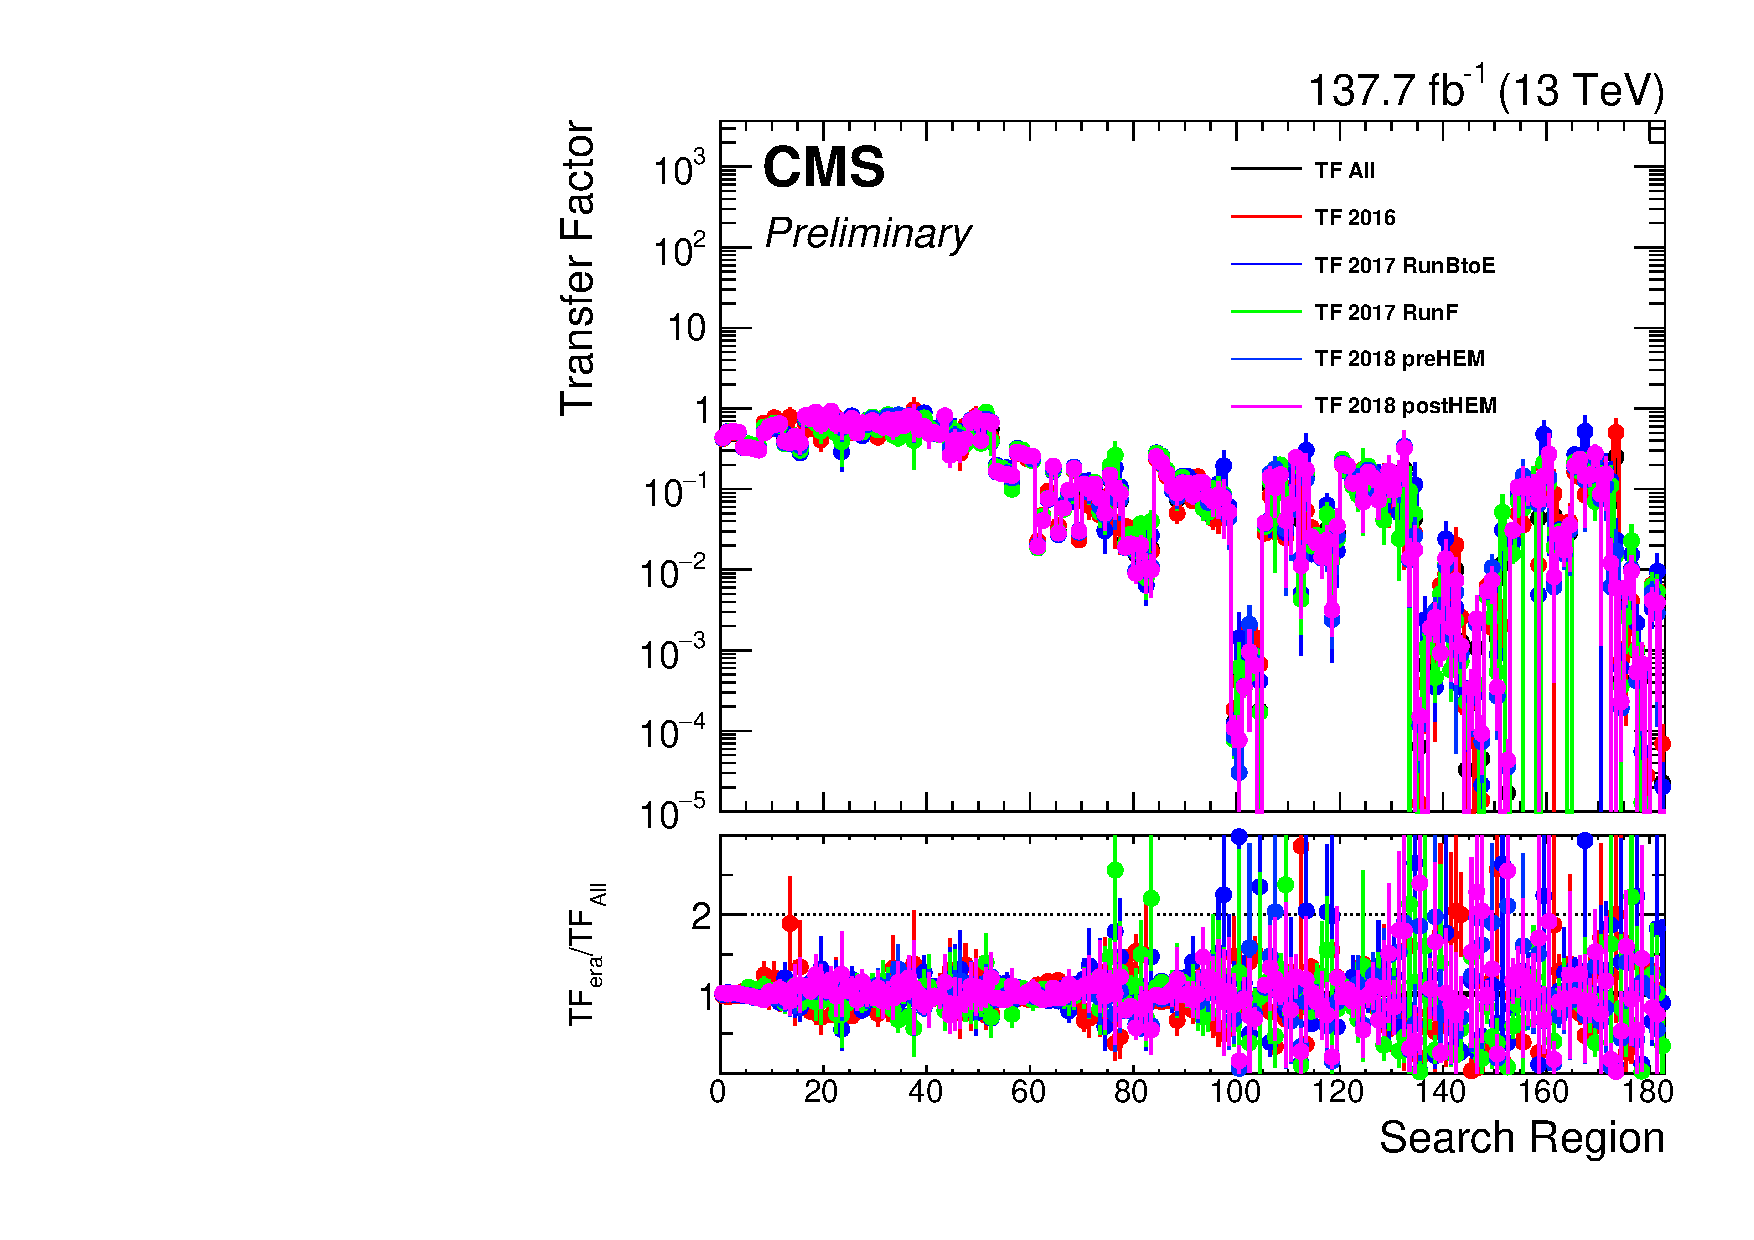
\includegraphics[width=0.4\textwidth]{LostLepton_TF_Comparison.pdf}
  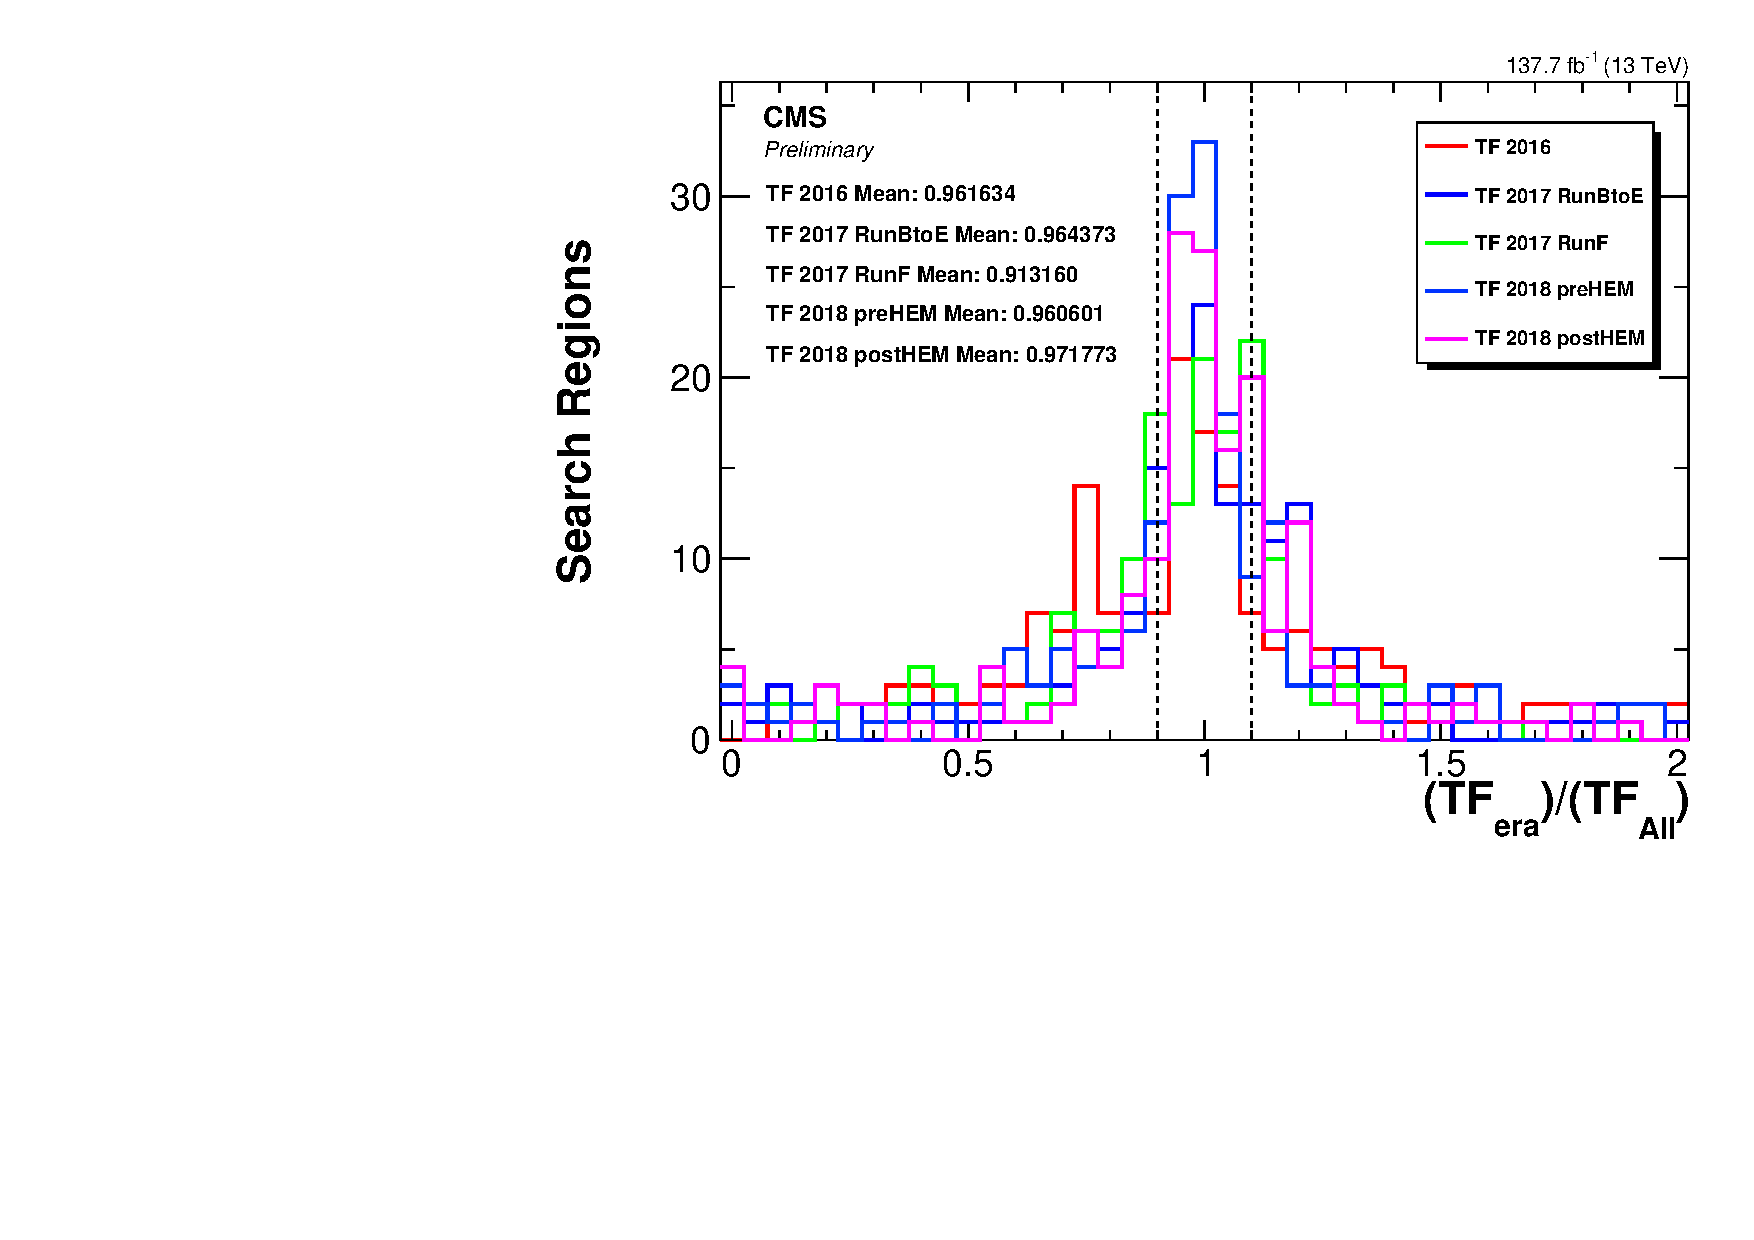
\includegraphics[width=0.5\textwidth]{LostLepton_TF_Comparison_sum.pdf} \\
	\end{center}
	\caption[Transfer Factor Comparison]{Comparisons of the transfer factors for each era of MC in the low and high \dm{} regions. The values are shown in their separate bins on the left plot and in a combined form on the right. The mean for each is also shown. 
	 }
	\label{fig:llb-1lcr-datavsmc-total-tf}
\end{figure}
\begin{figure}
	\begin{center}  
		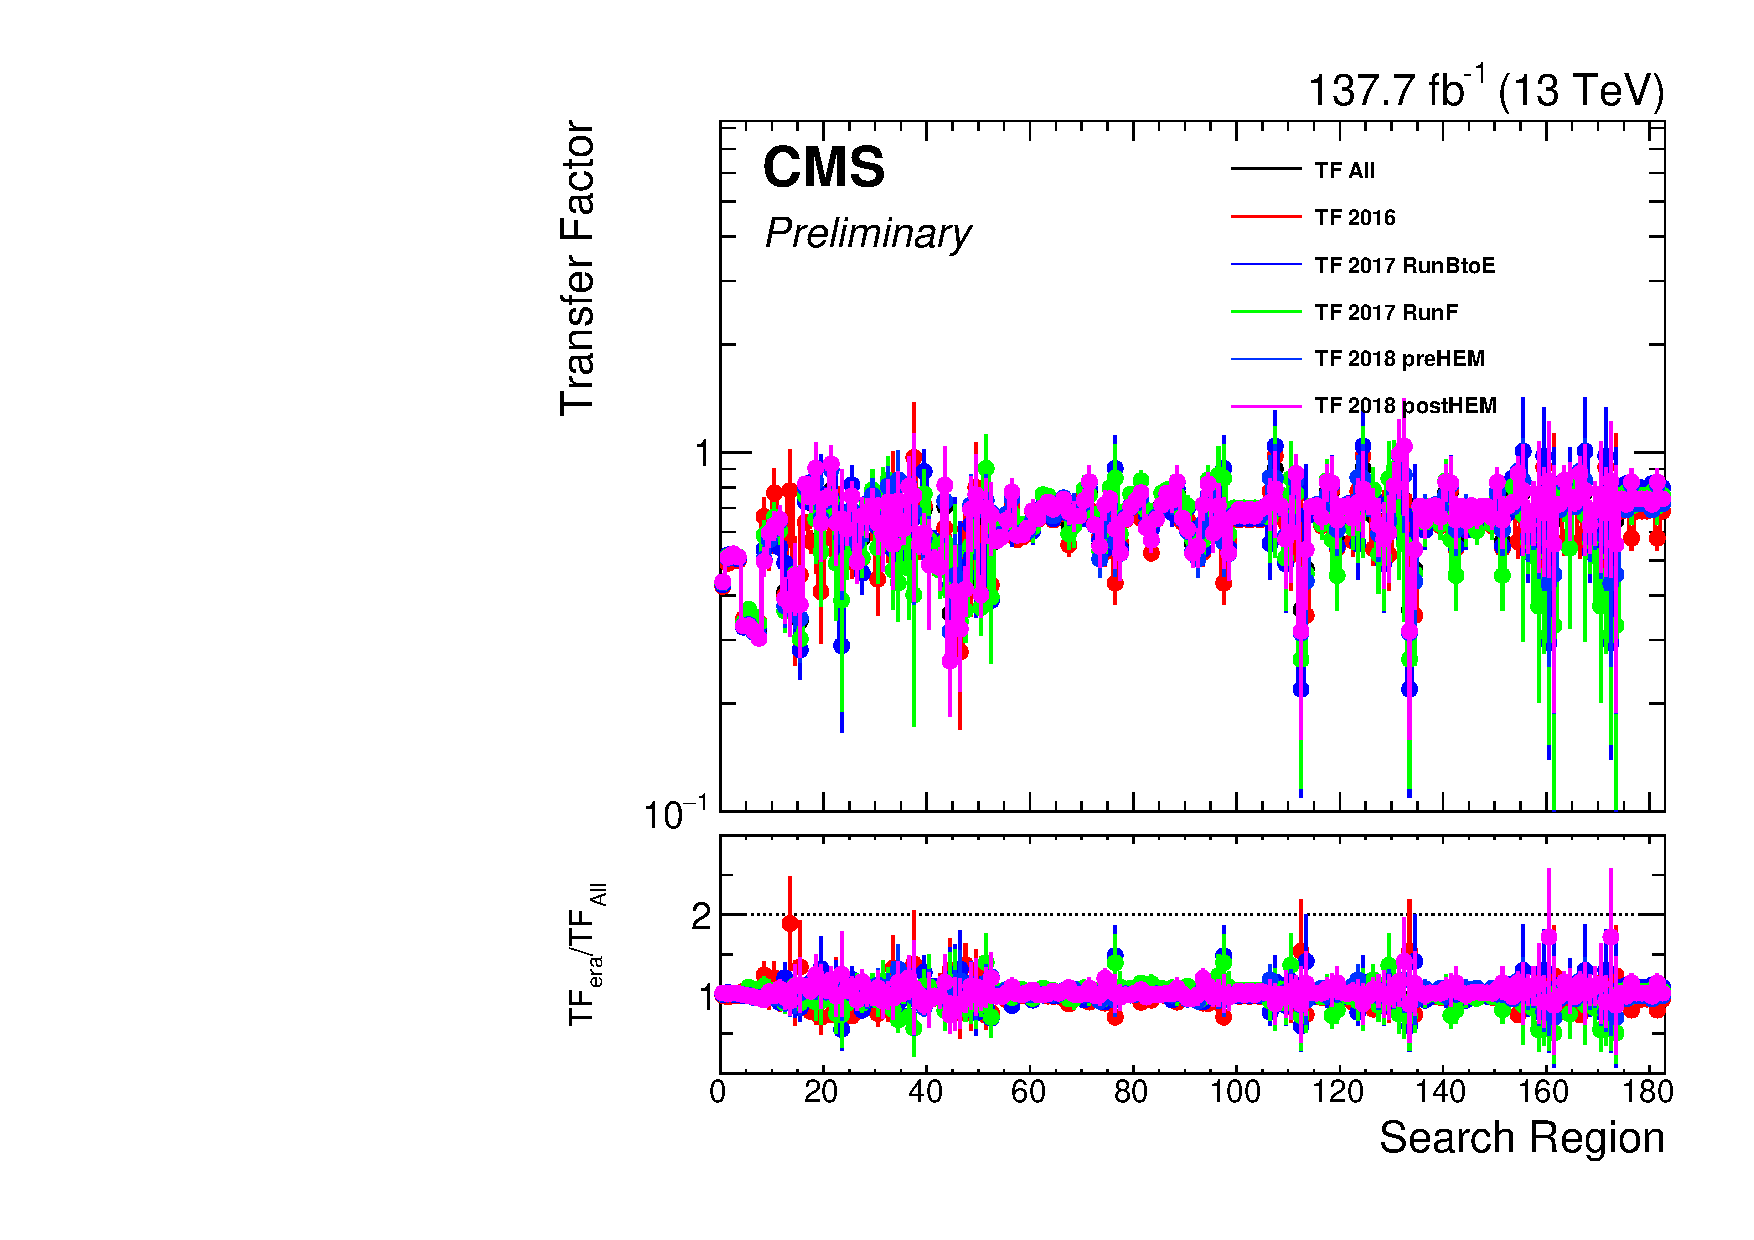
\includegraphics[width=0.4\textwidth]{LostLepton_TF_CR_to_SR_noextrap_Comparison.pdf}
		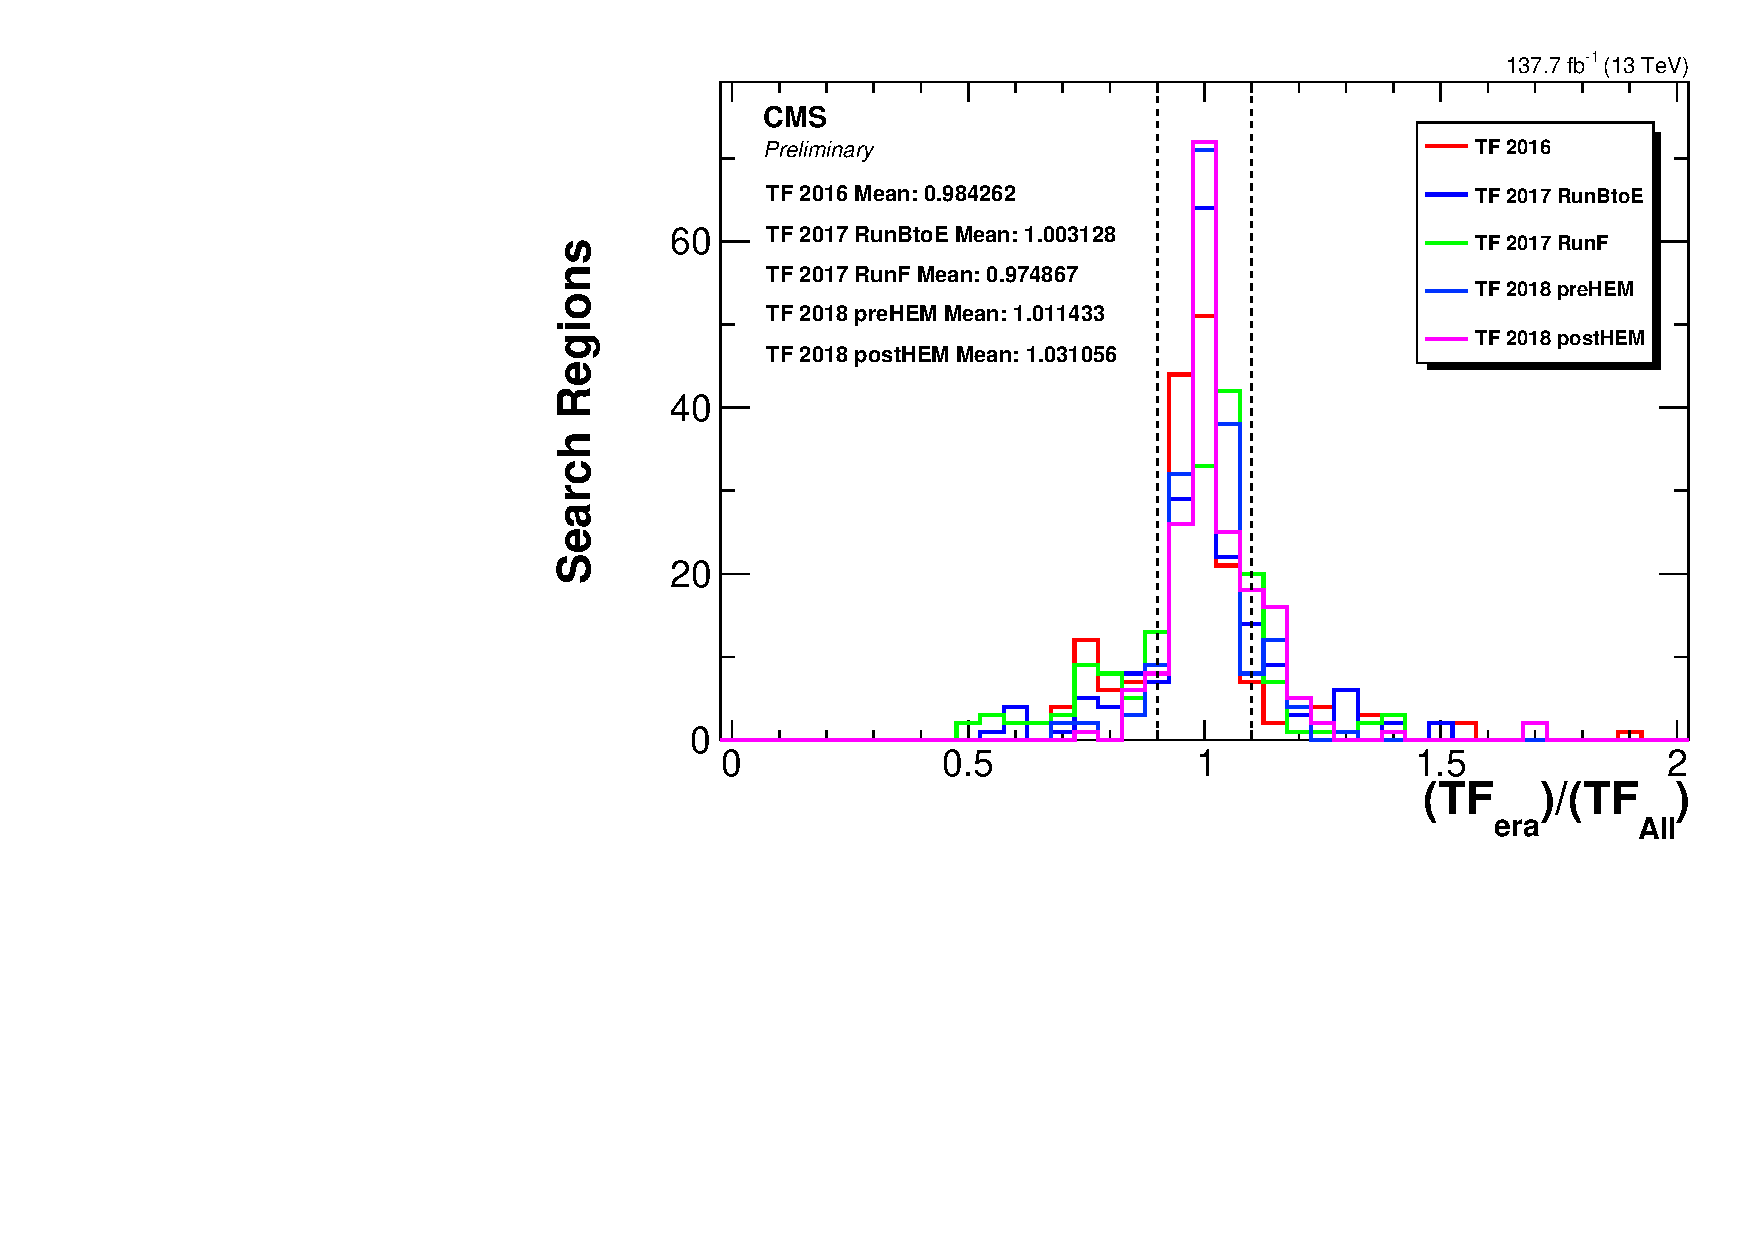
\includegraphics[width=0.5\textwidth]{LostLepton_TF_CR_to_SR_noextrap_Comparison_sum.pdf} \\
		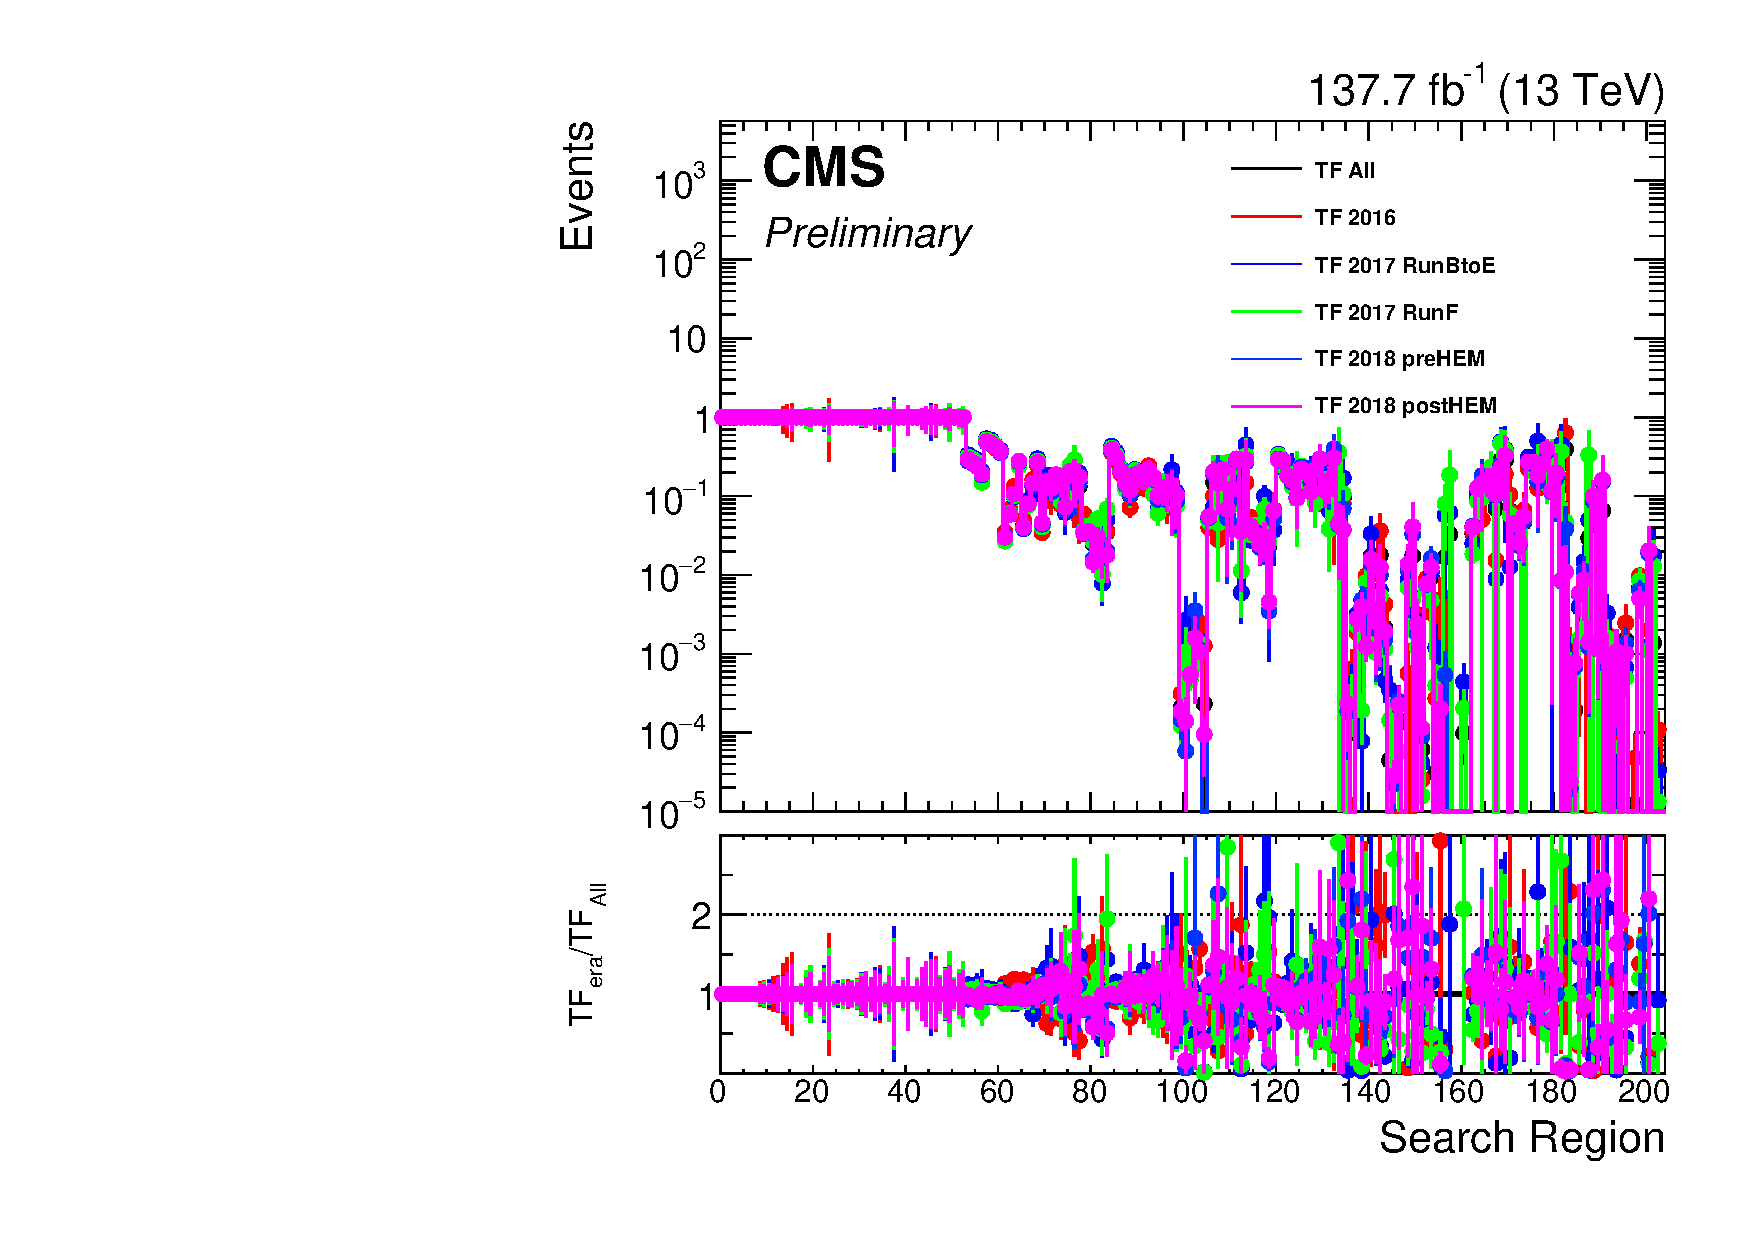
\includegraphics[width=0.4\textwidth]{LostLepton_TF_SR_extrap_Comparison.pdf}
		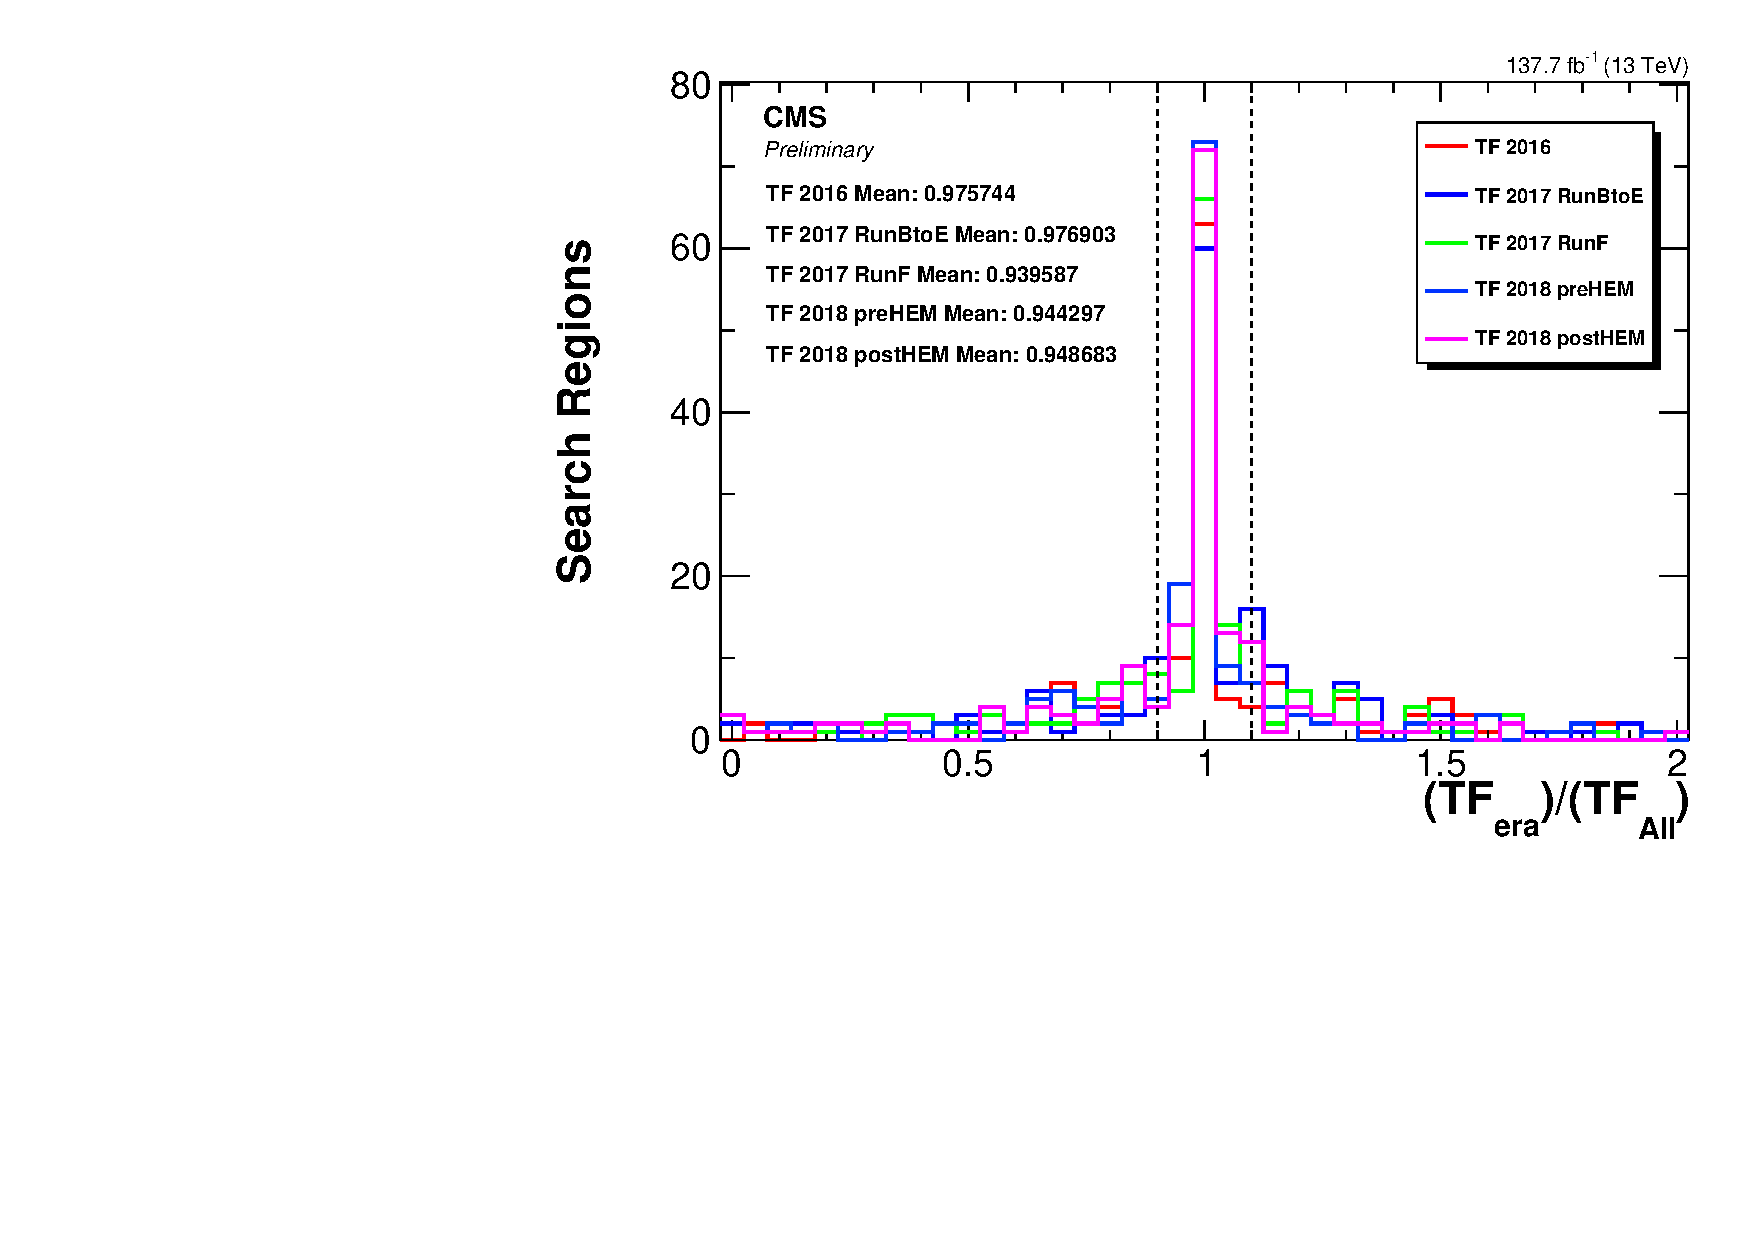
\includegraphics[width=0.5\textwidth]{LostLepton_TF_SR_extrap_Comparison_sum.pdf}
	\end{center}
	\caption[Separated Transfer Factor Comparison]{Comparisons of the transfer factors, separated into the CR-to-SR (top) and SR-to-extrapolation (bottom), for each era of MC in the low and high \dm{} regions. The values are shown in their separate bins on the left plot and in a combined form on the right. The mean for each is also shown. 
	 }
	\label{fig:llb-1lcr-datavsmc-sep-tf}
\end{figure}

% matches pred table
% copy and paste the output from the end of LLBPred() (it calls printMoriond17Table) between the below labels "start insert" and "stop insert".
\begin{table}[!!htbp]
\begin{center}
\resizebox*{0.6\textwidth}{!}{
\begin{tabular}{|c||c||c|c|c|}
\hline
Search Region & \met [GeV] & $N_{\text{data}}(1l)$ & $\tfll$ & $N_\text{pred}^{\text{LL}}$ \\
\hline
% Search region & 	$\met$ & 	singlelep & 	_TF & 	_pred & 	
\hline
\multicolumn{5}{c}{low \dm, $\nb=0$, $\nsv=0$, $\ptisr\geq500$\,GeV, $2\leq\nj\leq5$} \\
\hline
 %  lm_nb0_nivf0_highptisr_nj2to5
0 & 450$-$550 & 	5045 & 	0.432$\pm$0.004 & 	2178.23$\pm$35.68 \\
1 & 550$-$650 & 	2198 & 	0.509$\pm$0.004 & 	1118.77$\pm$25.67 \\
2 & 650$-$750 & 	818 & 	0.516$\pm$0.004 & 	421.97$\pm$15.16 \\
3 & $\geq750$ & 	540 & 	0.509$\pm$0.004 & 	274.59$\pm$12.04 \\
\hline
\multicolumn{5}{c}{low \dm, $\nb=0$, $\nsv=0$, $\ptisr\geq500$\,GeV, $\nj\geq6$} \\
\hline
 %     lm_nb0_nivf0_highptisr_nj6
4 & 450$-$550 & 	849 & 	0.333$\pm$0.004 & 	282.81$\pm$10.32 \\
5 & 550$-$650 & 	408 & 	0.338$\pm$0.005 & 	137.77$\pm$7.14 \\
6 & 650$-$750 & 	181 & 	0.331$\pm$0.006 & 	59.90$\pm$4.60 \\
7 & $\geq750$ & 	156 & 	0.321$\pm$0.006 & 	50.12$\pm$4.11 \\
\hline
\multicolumn{5}{c}{low \dm, $\nb=0$, $\nsv\geq1$, $\ptisr\geq500$\,GeV, $2\leq\nj\leq5$} \\
\hline
 %  lm_nb0_nivf1_highptisr_nj2to5
8 & 450$-$550 & 	148 & 	0.537$\pm$0.024 & 	79.42$\pm$7.44 \\
9 & 550$-$650 & 	38 & 	0.581$\pm$0.026 & 	22.09$\pm$3.71 \\
10 & 650$-$750 & 	25 & 	0.641$\pm$0.032 & 	16.03$\pm$3.31 \\
11 & $\geq750$ & 	16 & 	0.609$\pm$0.027 & 	9.75$\pm$2.48 \\
\hline
\multicolumn{5}{c}{low \dm, $\nb=0$, $\nsv\geq1$, $\ptisr\geq500$\,GeV, $\nj\geq6$} \\
\hline
 %     lm_nb0_nivf1_highptisr_nj6
12 & 450$-$550 & 	43 & 	0.410$\pm$0.028 & 	17.64$\pm$2.96 \\
13 & 550$-$650 & 	12 & 	0.415$\pm$0.037 & 	4.98$\pm$1.50 \\
14 & 650$-$750 & 	5 & 	0.414$\pm$0.040 & 	2.07$\pm$0.95 \\
15 & $\geq750$ & 	4 & 	0.341$\pm$0.041 & 	1.36$\pm$0.70 \\
\hline
\multicolumn{5}{c}{low \dm, $\nb=1$, $\nsv=0$, $\mtb<175$~\GeV, $300\leq\ptisr<500$\,GeV, $\ptb<40$\,GeV} \\
\hline
 % lm_nb1_nivf0_lowmtb_lowptisr_lowptb
16 & 300$-$400 & 	2037 & 	0.746$\pm$0.015 & 	1520.34$\pm$45.84 \\
17 & 400$-$500 & 	341 & 	0.724$\pm$0.031 & 	246.78$\pm$16.96 \\
18 & 500$-$600 & 	32 & 	0.726$\pm$0.061 & 	23.24$\pm$4.55 \\
19 & $\geq600$ & 	6 & 	0.581$\pm$0.068 & 	3.48$\pm$1.48 \\
\hline
\multicolumn{5}{c}{low \dm, $\nb=1$, $\nsv=0$, $\mtb<175$~\GeV, $300\leq\ptisr<500$\,GeV, $40<\ptb<70$\,GeV} \\
\hline
 % lm_nb1_nivf0_lowmtb_lowptisr_medptb
20 & 300$-$400 & 	1015 & 	0.716$\pm$0.019 & 	726.30$\pm$29.71 \\
21 & 400$-$500 & 	127 & 	0.786$\pm$0.047 & 	99.84$\pm$10.68 \\
22 & 500$-$600 & 	11 & 	0.655$\pm$0.076 & 	7.21$\pm$2.33 \\
23 & $\geq600$ & 	6 & 	0.524$\pm$0.115 & 	3.15$\pm$1.46 \\
\hline
\multicolumn{5}{c}{low \dm, $\nb=1$, $\nsv=0$, $\mtb<175$~\GeV, $\ptisr\geq500$\,GeV, $\ptb<40$\,GeV} \\
\hline
 % lm_nb1_nivf0_lowmtb_highptisr_lowptb
24 & 450$-$550 & 	136 & 	0.579$\pm$0.027 & 	78.76$\pm$7.72 \\
25 & 550$-$650 & 	45 & 	0.686$\pm$0.034 & 	30.87$\pm$4.85 \\
26 & 650$-$750 & 	12 & 	0.537$\pm$0.033 & 	6.44$\pm$1.90 \\
27 & $\geq750$ & 	14 & 	0.576$\pm$0.034 & 	8.07$\pm$2.21 \\
\hline
\multicolumn{5}{c}{low \dm, $\nb=1$, $\nsv=0$, $\mtb<175$~\GeV, $\ptisr\geq500$\,GeV, $40<\ptb<70$\,GeV} \\
\hline
 % lm_nb1_nivf0_lowmtb_highptisr_medptb
28 & 450$-$550 & 	89 & 	0.676$\pm$0.039 & 	60.14$\pm$7.25 \\
29 & 550$-$650 & 	19 & 	0.722$\pm$0.045 & 	13.72$\pm$3.26 \\
30 & 650$-$750 & 	11 & 	0.589$\pm$0.053 & 	6.47$\pm$2.04 \\
31 & $\geq750$ & 	3 & 	0.654$\pm$0.066 & 	1.96$\pm$1.15 \\
\hline
\multicolumn{5}{c}{low \dm, $\nb=1$, $\nsv\geq1$, $\mtb<175$~\GeV, $\ptb<40$\,GeV} \\
\hline
 %     lm_nb1_nivf1_lowmtb_lowptb
32 & 300$-$400 & 	115 & 	0.741$\pm$0.054 & 	85.23$\pm$10.10 \\
33 & 400$-$500 & 	26 & 	0.587$\pm$0.069 & 	15.26$\pm$3.49 \\
34 & $\geq500$ & 	13 & 	0.640$\pm$0.071 & 	8.32$\pm$2.49 \\
\hline
\multicolumn{5}{c}{low \dm, $\nb\geq2$, $\mtb<175$~\GeV, $300\leq\ptisr<500$\,GeV, $\ptbonetwo<80$\,GeV} \\
\hline
 % lm_nb2_lowmtb_lowptisr_lowptb12
35 & 300$-$400 & 	242 & 	0.603$\pm$0.028 & 	145.92$\pm$11.59 \\
36 & 400$-$500 & 	36 & 	0.667$\pm$0.066 & 	24.00$\pm$4.65 \\
37 & $\geq500$ & 	7 & 	0.704$\pm$0.169 & 	4.93$\pm$2.21 \\
\hline
\multicolumn{5}{c}{low \dm, $\nb\geq2$, $\mtb<175$~\GeV, $300\leq\ptisr<500$\,GeV, $80<\ptbonetwo<140$\,GeV} \\
\hline
 % lm_nb2_lowmtb_lowptisr_medptb12
38 & 300$-$400 & 	579 & 	0.554$\pm$0.015 & 	320.86$\pm$15.79 \\
39 & 400$-$500 & 	101 & 	0.694$\pm$0.045 & 	70.12$\pm$8.31 \\
40 & $\geq500$ & 	16 & 	0.525$\pm$0.081 & 	8.40$\pm$2.47 \\
\hline
\multicolumn{5}{c}{low \dm, $\nb\geq2$, $\mtb<175$~\GeV, $300\leq\ptisr<500$\,GeV, $\ptbonetwo\geq140$\,GeV, $\nj\geq7$} \\
\hline
 % lm_nb2_lowmtb_lowptisr_highptb12_nj7
41 & 300$-$400 & 	318 & 	0.516$\pm$0.016 & 	164.19$\pm$10.49 \\
42 & 400$-$500 & 	53 & 	0.494$\pm$0.031 & 	26.19$\pm$3.96 \\
43 & $\geq500$ & 	9 & 	0.706$\pm$0.088 & 	6.36$\pm$2.26 \\
\hline
\multicolumn{5}{c}{low \dm, $\nb\geq2$, $\mtb<175$~\GeV, $\ptisr\geq500$\,GeV, $\ptbonetwo<80$\,GeV} \\
\hline
 % lm_nb2_lowmtb_highptisr_lowptb12
44 & 450$-$550 & 	19 & 	0.356$\pm$0.047 & 	6.77$\pm$1.79 \\
45 & 550$-$650 & 	7 & 	0.469$\pm$0.075 & 	3.29$\pm$1.35 \\
46 & $\geq650$ & 	2 & 	0.366$\pm$0.057 & 	0.73$\pm$0.53 \\
\hline
\multicolumn{5}{c}{low \dm, $\nb\geq2$, $\mtb<175$~\GeV, $\ptisr\geq500$\,GeV, $80<\ptbonetwo<140$\,GeV} \\
\hline
 % lm_nb2_lowmtb_highptisr_medptb12
47 & 450$-$550 & 	50 & 	0.447$\pm$0.035 & 	22.33$\pm$3.60 \\
48 & 550$-$650 & 	16 & 	0.631$\pm$0.074 & 	10.10$\pm$2.79 \\
49 & $\geq650$ & 	6 & 	0.699$\pm$0.103 & 	4.20$\pm$1.82 \\
\hline
\multicolumn{5}{c}{low \dm, $\nb\geq2$, $\mtb<175$~\GeV, $\ptisr\geq500$\,GeV, $\ptbonetwo\geq140$\,GeV, $\nj\geq7$} \\
\hline
 % lm_nb2_lowmtb_highptisr_highptb12_nj7
50 & 450$-$550 & 	59 & 	0.429$\pm$0.027 & 	25.31$\pm$3.67 \\
51 & 550$-$650 & 	19 & 	0.649$\pm$0.063 & 	12.32$\pm$3.07 \\
52 & $\geq650$ & 	7 & 	0.559$\pm$0.070 & 	3.91$\pm$1.56 \\
\hline
\end{tabular}
}
\caption{\label{tab:0l-llb-pred-lm}The LL estimate in the various low \dm{} search regions, bins 0 to 53, using the \datalumi~dataset.}
\end{center}
\end{table}
% matches pred table
% copy and paste the output from the end of LLBPred() (it calls printMoriond17Table) between the below labels "start insert" and "stop insert".
\begin{table}[!h]
\begin{center}
\resizebox*{0.6\textwidth}{!}{
\begin{tabular}{|c||c||c|c|c|c|c|}
\hline
Search Region & \met [GeV] & $N_{\text{data}}(1l)$ & $\tfll$ & $\tfll^{\text{CR-SR}}$ & $\tfll^{\text{SR-extrap}}$ & $N_\text{pred}^{\text{LL}}$ \\
\hline
% Search region & 	$\met$ & 	singlelep & 	_TF & 	_TF_CR_to_SR_noextrap & 	_TF_SR_extrap & 	_pred & 	
\hline
\multicolumn{7}{c}{high \dm, $\nb=1$, $\mtb<175$~\GeV, $\nj\geq7$, $\nrt\geq1$} \\
\hline
 %      hm_nb1_lowmtb_nj7_nrtgeq1
53 & 250$-$300 & 	1151 & 	0.196$\pm$0.004 & 	0.519 & 	0.378 & 	225.43$\pm$8.24 \\
54 & 300$-$400 & 	697 & 	0.187$\pm$0.005 & 	0.550 & 	0.340 & 	130.35$\pm$6.21 \\
55 & 400$-$500 & 	129 & 	0.180$\pm$0.011 & 	0.577 & 	0.313 & 	23.26$\pm$2.53 \\
56 & $\geq500$ & 	43 & 	0.157$\pm$0.016 & 	0.598 & 	0.263 & 	6.77$\pm$1.25 \\
\hline
\multicolumn{7}{c}{high \dm, $\nb\geq2$, $\mtb<175$~\GeV, $\nj\geq7$, $\nrt\geq1$} \\
\hline
 %      hm_nb2_lowmtb_nj7_nrtgeq1
57 & 250$-$300 & 	2250 & 	0.292$\pm$0.004 & 	0.539 & 	0.542 & 	657.73$\pm$16.12 \\
58 & 300$-$400 & 	1256 & 	0.286$\pm$0.005 & 	0.548 & 	0.522 & 	359.11$\pm$11.69 \\
59 & 400$-$500 & 	236 & 	0.278$\pm$0.010 & 	0.582 & 	0.478 & 	65.56$\pm$4.92 \\
60 & $\geq500$ & 	99 & 	0.259$\pm$0.017 & 	0.625 & 	0.415 & 	25.67$\pm$3.06 \\
\hline
\multicolumn{7}{c}{high \dm, $\nb=1$, $\mtb\geq175$~\GeV, $\nt=0$, $\nrt=0$, $\nw=0$, $\Ht\geq1000$} \\
\hline
 % hm_nb1_highmtb_nt0_nrt0_nw0_htgt1000
61 & 250$-$350 & 	570 & 	0.383$\pm$0.007 & 	0.657 & 	0.583 & 	218.28$\pm$10.01 \\
62 & 350$-$450 & 	233 & 	0.369$\pm$0.011 & 	0.614 & 	0.602 & 	86.03$\pm$6.16 \\
63 & 450$-$550 & 	102 & 	0.362$\pm$0.015 & 	0.544 & 	0.666 & 	36.97$\pm$3.96 \\
64 & $\geq550$ & 	109 & 	0.352$\pm$0.013 & 	0.531 & 	0.663 & 	38.39$\pm$3.93 \\
\hline
\multicolumn{7}{c}{high \dm, $\nb\geq2$, $\mtb\geq175$~\GeV, $\nt=0$, $\nrt=0$, $\nw=0$, $\Ht\geq1000$} \\
\hline
 % hm_nb2_highmtb_nt0_nrt0_nw0_htgt1000
65 & 250$-$350 & 	186 & 	0.359$\pm$0.013 & 	0.738 & 	0.486 & 	66.78$\pm$5.49 \\
66 & 350$-$450 & 	57 & 	0.379$\pm$0.021 & 	0.675 & 	0.561 & 	21.58$\pm$3.11 \\
67 & 450$-$550 & 	23 & 	0.334$\pm$0.027 & 	0.616 & 	0.542 & 	7.69$\pm$1.72 \\
68 & $\geq550$ & 	32 & 	0.317$\pm$0.025 & 	0.537 & 	0.590 & 	10.14$\pm$1.97 \\
\hline
\multicolumn{7}{c}{high \dm, $\nb=1$, $\mtb\geq175$~\GeV, $\nt\geq1$, $\nrt=0$, $\nw=0$, $\Ht<1000$} \\
\hline
 % hm_nb1_highmtb_ntgeq1_nrt0_nw0_htlt1000
69 & 250$-$550 & 	11329 & 	0.035$\pm$0.001 & 	0.601 & 	0.058 & 	397.77$\pm$7.71 \\
70 & 550$-$650 & 	87 & 	0.081$\pm$0.010 & 	0.553 & 	0.147 & 	7.07$\pm$1.14 \\
71 & $\geq650$ & 	29 & 	0.075$\pm$0.015 & 	0.684 & 	0.110 & 	2.18$\pm$0.59 \\
\hline
\multicolumn{7}{c}{high \dm, $\nb=1$, $\mtb\geq175$~\GeV, $\nt\geq1$, $\nrt=0$, $\nw=0$, $1000\leq\Ht<1500$} \\
\hline
 % hm_nb1_highmtb_ntgeq1_nrt0_nw0_ht1000to1500
72 & 250$-$550 & 	739 & 	0.111$\pm$0.004 & 	0.621 & 	0.179 & 	81.90$\pm$4.07 \\
73 & 550$-$650 & 	36 & 	0.063$\pm$0.011 & 	0.507 & 	0.125 & 	2.27$\pm$0.55 \\
74 & $\geq650$ & 	42 & 	0.053$\pm$0.011 & 	0.539 & 	0.098 & 	2.23$\pm$0.56 \\
\hline
\multicolumn{7}{c}{high \dm, $\nb=1$, $\mtb\geq175$~\GeV, $\nt\geq1$, $\nrt=0$, $\nw=0$, $\Ht\geq1500$} \\
\hline
 % hm_nb1_highmtb_ntgeq1_nrt0_nw0_htgt1500
75 & 250$-$550 & 	166 & 	0.131$\pm$0.008 & 	0.690 & 	0.190 & 	21.70$\pm$2.19 \\
76 & 550$-$650 & 	8 & 	0.124$\pm$0.030 & 	0.637 & 	0.195 & 	0.99$\pm$0.43 \\
77 & $\geq650$ & 	23 & 	0.079$\pm$0.019 & 	0.506 & 	0.156 & 	1.81$\pm$0.57 \\
\hline
\multicolumn{7}{c}{high \dm, $\nb=1$, $\mtb\geq175$~\GeV, $\nt=0$, $\nrt=0$, $\nw\geq1$, $\Ht<1300$} \\
\hline
 % hm_nb1_highmtb_nt0_nrt0_nwgeq1_htlt1300
78 & 250$-$350 & 	9720 & 	0.023$\pm$0.000 & 	0.594 & 	0.038 & 	220.56$\pm$5.06 \\
79 & 350$-$450 & 	1773 & 	0.023$\pm$0.001 & 	0.638 & 	0.036 & 	40.40$\pm$2.18 \\
80 & $\geq450$ & 	586 & 	0.015$\pm$0.001 & 	0.612 & 	0.025 & 	9.07$\pm$0.94 \\
\hline
\multicolumn{7}{c}{high \dm, $\nb=1$, $\mtb\geq175$~\GeV, $\nt=0$, $\nrt=0$, $\nw\geq1$, $\Ht\geq1300$} \\
\hline
 % hm_nb1_highmtb_nt0_nrt0_nwgeq1_htgt1300
81 & 250$-$350 & 	206 & 	0.023$\pm$0.003 & 	0.718 & 	0.032 & 	4.67$\pm$0.68 \\
82 & 350$-$450 & 	87 & 	0.011$\pm$0.002 & 	0.607 & 	0.018 & 	0.94$\pm$0.22 \\
83 & $\geq450$ & 	87 & 	0.021$\pm$0.004 & 	0.545 & 	0.038 & 	1.82$\pm$0.37 \\
\hline
\multicolumn{7}{c}{high \dm, $\nb=1$, $\mtb\geq175$~\GeV, $\nt=0$, $\nrt\geq1$, $\nw=0$, $\Ht<1000$} \\
\hline
 % hm_nb1_highmtb_nt0_nrtgeq1_nw0_htlt1000
84 & 250$-$350 & 	9356 & 	0.253$\pm$0.002 & 	0.592 & 	0.427 & 	2362.92$\pm$30.67 \\
85 & 350$-$450 & 	1627 & 	0.227$\pm$0.004 & 	0.640 & 	0.355 & 	369.27$\pm$11.50 \\
86 & 450$-$550 & 	346 & 	0.169$\pm$0.007 & 	0.652 & 	0.259 & 	58.49$\pm$4.01 \\
87 & 550$-$650 & 	87 & 	0.123$\pm$0.011 & 	0.553 & 	0.223 & 	10.73$\pm$1.49 \\
88 & $\geq650$ & 	29 & 	0.118$\pm$0.017 & 	0.684 & 	0.173 & 	3.44$\pm$0.80 \\
\hline
\multicolumn{7}{c}{high \dm, $\nb=1$, $\mtb\geq175$~\GeV, $\nt=0$, $\nrt\geq1$, $\nw=0$, $1000\leq\Ht<1500$} \\
\hline
 % hm_nb1_highmtb_nt0_nrtgeq1_nw0_ht1000to1500
89 & 250$-$350 & 	470 & 	0.126$\pm$0.005 & 	0.639 & 	0.198 & 	59.43$\pm$3.64 \\
90 & 350$-$450 & 	187 & 	0.128$\pm$0.008 & 	0.619 & 	0.207 & 	23.93$\pm$2.35 \\
91 & 450$-$550 & 	82 & 	0.089$\pm$0.009 & 	0.520 & 	0.171 & 	7.28$\pm$1.11 \\
92 & 550$-$650 & 	36 & 	0.121$\pm$0.016 & 	0.507 & 	0.239 & 	4.36$\pm$0.93 \\
93 & $\geq650$ & 	42 & 	0.086$\pm$0.011 & 	0.539 & 	0.160 & 	3.61$\pm$0.73 \\
\hline
\end{tabular}
}
\caption[LL HM CR bins 53-93]{\label{tab:0l-llb-pred-hm-1}The LL estimate in the various high \dm{} search regions, bins 53 to 93, using the \datalumi~dataset.}
\end{center}
\end{table}
% matches pred table
% copy and paste the output from the end of LLBPred() (it calls printMoriond17Table) between the below labels "start insert" and "stop insert".
\begin{table}[!h]
\begin{center}
\resizebox*{0.6\textwidth}{!}{
\begin{tabular}{|c||c||c|c|c|c|c|}
\hline
Search Region & \met [GeV] & $N_{\text{data}}(1l)$ & $\tfll$ & $\tfll^{\text{CR-SR}}$ & $\tfll^{\text{SR-extrap}}$ & $N_\text{pred}^{\text{LL}}$ \\
\hline
\multicolumn{7}{c}{high \dm, $\nb=1$, $\mtb\geq175$~\GeV, $\nt=0$, $\nrt\geq1$, $\nw=0$, $\Ht\geq1500$} \\
\hline
 % hm_nb1_highmtb_nt0_nrtgeq1_nw0_htgt1500
94 & 250$-$350 & 	100 & 	0.075$\pm$0.008 & 	0.744 & 	0.100 & 	7.46$\pm$1.06 \\
95 & 350$-$450 & 	46 & 	0.069$\pm$0.011 & 	0.589 & 	0.118 & 	3.19$\pm$0.68 \\
96 & 450$-$550 & 	20 & 	0.087$\pm$0.017 & 	0.649 & 	0.135 & 	1.75$\pm$0.52 \\
97 & 550$-$650 & 	8 & 	0.101$\pm$0.029 & 	0.637 & 	0.158 & 	0.80$\pm$0.37 \\
98 & $\geq650$ & 	23 & 	0.040$\pm$0.011 & 	0.506 & 	0.079 & 	0.92$\pm$0.31 \\
\hline
\multicolumn{7}{c}{high \dm, $\nb=1$, $\mtb\geq175$~\GeV, $\nt\geq1$, $\nrt=0$, $\nw\geq1$} \\
\hline
 % hm_nb1_highmtb_ntgeq1_nrt0_nwgeq1
99 & 250$-$550 & 	12234 & 	0.000$\pm$0.000 & 	0.604 & 	0.000 & 	2.42$\pm$0.44 \\
100 & $\geq550$ & 	225 & 	0.001$\pm$0.000 & 	0.557 & 	0.001 & 	0.16$\pm$0.10 \\
\hline
\multicolumn{7}{c}{high \dm, $\nb=1$, $\mtb\geq175$~\GeV, $\nt\geq1$, $\nrt\geq1$, $\nw=0$} \\
\hline
 % hm_nb1_highmtb_ntgeq1_nrtgeq1_nw0
101 & 250$-$550 & 	12234 & 	0.001$\pm$0.000 & 	0.604 & 	0.001 & 	6.76$\pm$0.80 \\
102 & $\geq550$ & 	225 & 	0.002$\pm$0.001 & 	0.557 & 	0.003 & 	0.35$\pm$0.13 \\
\hline
\multicolumn{7}{c}{high \dm, $\nb=1$, $\mtb\geq175$~\GeV, $\nt=0$, $\nrt\geq1$, $\nw\geq1$} \\
\hline
 % hm_nb1_highmtb_nt0_nrtgeq1_nwgeq1
103 & 250$-$550 & 	12234 & 	0.001$\pm$0.000 & 	0.604 & 	0.002 & 	17.29$\pm$1.17 \\
104 & $\geq550$ & 	225 & 	0.000$\pm$0.000 & 	0.557 & 	0.001 & 	0.08$\pm$0.07 \\
\hline
\multicolumn{7}{c}{high \dm, $\nb=2$, $\mtb\geq175$~\GeV, $\nt=1$, $\nrt=0$, $\nw=0$, $\Ht<1000$} \\
\hline
 % hm_nbeq2_highmtb_nt1_nrt0_nw0_htlt1000
105 & 250$-$550 & 	2055 & 	0.040$\pm$0.001 & 	0.650 & 	0.062 & 	82.37$\pm$3.55 \\
106 & 550$-$650 & 	15 & 	0.108$\pm$0.022 & 	0.614 & 	0.176 & 	1.62$\pm$0.53 \\
107 & $\geq650$ & 	7 & 	0.084$\pm$0.030 & 	0.737 & 	0.115 & 	0.59$\pm$0.31 \\
\hline
\multicolumn{7}{c}{high \dm, $\nb=2$, $\mtb\geq175$~\GeV, $\nt=1$, $\nrt=0$, $\nw=0$, $1000\leq\Ht<1500$} \\
\hline
 % hm_nbeq2_highmtb_nt1_nrt0_nw0_ht1000to1500
108 & 250$-$550 & 	151 & 	0.149$\pm$0.009 & 	0.710 & 	0.210 & 	22.56$\pm$2.25 \\
109 & 550$-$650 & 	7 & 	0.042$\pm$0.016 & 	0.521 & 	0.080 & 	0.29$\pm$0.15 \\
110 & $\geq650$ & 	13 & 	0.089$\pm$0.028 & 	0.539 & 	0.165 & 	1.16$\pm$0.48 \\
\hline
\multicolumn{7}{c}{high \dm, $\nb=2$, $\mtb\geq175$~\GeV, $\nt=1$, $\nrt=0$, $\nw=0$, $\Ht\geq1500$} \\
\hline
 % hm_nbeq2_highmtb_nt1_nrt0_nw0_htgt1500
111 & 250$-$550 & 	45 & 	0.202$\pm$0.022 & 	0.819 & 	0.246 & 	9.07$\pm$1.67 \\
112 & 550$-$650 & 	3 & 	0.052$\pm$0.035 & 	0.418 & 	0.126 & 	0.16$\pm$0.14 \\
113 & $\geq650$ & 	5 & 	0.134$\pm$0.044 & 	0.446 & 	0.301 & 	0.67$\pm$0.37 \\
\hline
\multicolumn{7}{c}{high \dm, $\nb=2$, $\mtb\geq175$~\GeV, $\nt=0$, $\nrt=0$, $\nw=1$, $\Ht<1300$} \\
\hline
 % hm_nbeq2_highmtb_nt0_nrt0_nw1_htlt1300
114 & 250$-$350 & 	1742 & 	0.025$\pm$0.001 & 	0.657 & 	0.038 & 	43.11$\pm$2.60 \\
115 & 350$-$450 & 	340 & 	0.023$\pm$0.002 & 	0.656 & 	0.036 & 	7.96$\pm$0.92 \\
116 & $\geq450$ & 	121 & 	0.014$\pm$0.003 & 	0.601 & 	0.023 & 	1.71$\pm$0.40 \\
\hline
\multicolumn{7}{c}{high \dm, $\nb=2$, $\mtb\geq175$~\GeV, $\nt=0$, $\nrt=0$, $\nw=1$, $\Ht\geq1300$} \\
\hline
 % hm_nbeq2_highmtb_nt0_nrt0_nw1_htgt1300
117 & 250$-$350 & 	52 & 	0.028$\pm$0.006 & 	0.793 & 	0.036 & 	1.47$\pm$0.38 \\
118 & 350$-$450 & 	21 & 	0.017$\pm$0.008 & 	0.828 & 	0.021 & 	0.36$\pm$0.19 \\
119 & $\geq450$ & 	25 & 	0.035$\pm$0.011 & 	0.566 & 	0.062 & 	0.87$\pm$0.33 \\
\hline
\multicolumn{7}{c}{high \dm, $\nb=2$, $\mtb\geq175$~\GeV, $\nt=0$, $\nrt=1$, $\nw=0$, $\Ht<1000$} \\
\hline
 % hm_nbeq2_highmtb_nt0_nrt1_nw0_htlt1000
120 & 250$-$350 & 	1661 & 	0.225$\pm$0.004 & 	0.651 & 	0.346 & 	373.86$\pm$11.68 \\
121 & 350$-$450 & 	317 & 	0.196$\pm$0.009 & 	0.659 & 	0.297 & 	62.06$\pm$4.44 \\
122 & 450$-$550 & 	77 & 	0.147$\pm$0.014 & 	0.605 & 	0.243 & 	11.32$\pm$1.69 \\
123 & 550$-$650 & 	15 & 	0.143$\pm$0.026 & 	0.614 & 	0.234 & 	2.15$\pm$0.68 \\
124 & $\geq650$ & 	7 & 	0.173$\pm$0.048 & 	0.737 & 	0.235 & 	1.21$\pm$0.57 \\
\hline
\multicolumn{7}{c}{high \dm, $\nb=2$, $\mtb\geq175$~\GeV, $\nt=0$, $\nrt=1$, $\nw=0$, $1000\leq\Ht<1500$} \\
\hline
 % hm_nbeq2_highmtb_nt0_nrt1_nw0_ht1000to1500
125 & 250$-$350 & 	105 & 	0.171$\pm$0.011 & 	0.752 & 	0.227 & 	17.91$\pm$2.12 \\
126 & 350$-$450 & 	30 & 	0.119$\pm$0.014 & 	0.663 & 	0.180 & 	3.57$\pm$0.78 \\
127 & 450$-$550 & 	16 & 	0.102$\pm$0.018 & 	0.590 & 	0.172 & 	1.63$\pm$0.49 \\
128 & 550$-$650 & 	7 & 	0.104$\pm$0.026 & 	0.521 & 	0.199 & 	0.73$\pm$0.33 \\
129 & $\geq650$ & 	13 & 	0.110$\pm$0.028 & 	0.539 & 	0.204 & 	1.43$\pm$0.54 \\
\hline
\multicolumn{7}{c}{high \dm, $\nb=2$, $\mtb\geq175$~\GeV, $\nt=0$, $\nrt=1$, $\nw=0$, $\Ht\geq1500$} \\
\hline
 % hm_nbeq2_highmtb_nt0_nrt1_nw0_htgt1500
130 & 250$-$350 & 	28 & 	0.125$\pm$0.020 & 	0.812 & 	0.154 & 	3.49$\pm$0.87 \\
131 & 350$-$450 & 	14 & 	0.090$\pm$0.024 & 	0.844 & 	0.106 & 	1.26$\pm$0.48 \\
132 & 450$-$550 & 	3 & 	0.194$\pm$0.064 & 	0.800 & 	0.243 & 	0.58$\pm$0.39 \\
133 & 550$-$650 & 	3 & 	0.094$\pm$0.052 & 	0.418 & 	0.225 & 	0.28$\pm$0.23 \\
134 & $\geq650$ & 	5 & 	0.044$\pm$0.020 & 	0.446 & 	0.099 & 	0.22$\pm$0.14 \\
\hline
\end{tabular}
}
\caption[LL HM CR bins 94-134]{\label{tab:0l-llb-pred-hm-2}The LL estimate in the various high \dm{} search regions, bins 94 to 134, using the \datalumi~dataset.}
\end{center}
\end{table}
% matches pred table
% copy and paste the output from the end of LLBPred() (it calls printMoriond17Table) between the below labels "start insert" and "stop insert".
\begin{table}[!h]
\begin{center}
\resizebox*{0.6\textwidth}{!}{
\begin{tabular}{|c||c||c|c|c|c|c|}
\hline
Search Region & \met [GeV] & $N_{\text{data}}(1l)$ & $\tfll$ & $\tfll^{\text{CR-SR}}$ & $\tfll^{\text{SR-extrap}}$ & $N_\text{pred}^{\text{LL}}$ \\
\hline
\multicolumn{7}{c}{high \dm, $\nb=2$, $\mtb\geq175$~\GeV, $\nt=1$, $\nrt=0$, $\nw=1$} \\
\hline
 %  hm_nbeq2_highmtb_nt1_nrt0_nw1
135 & 250$-$550 & 	2251 & 	0.000$\pm$0.000 & 	0.659 & 	0.000 & 	0.21$\pm$0.09 \\
136 & $\geq550$ & 	50 & 	0.001$\pm$0.001 & 	0.566 & 	0.001 & 	0.04$\pm$0.03 \\
\hline
\multicolumn{7}{c}{high \dm, $\nb=2$, $\mtb\geq175$~\GeV, $\nt=1$, $\nrt=1$, $\nw=0$, $\Ht<1300$} \\
\hline
 % hm_nbeq2_highmtb_nt1_nrt1_nw0_htlt1300
137 & 250$-$350 & 	1742 & 	0.003$\pm$0.000 & 	0.657 & 	0.004 & 	4.39$\pm$0.66 \\
138 & 350$-$450 & 	340 & 	0.002$\pm$0.001 & 	0.656 & 	0.003 & 	0.72$\pm$0.22 \\
139 & $\geq450$ & 	121 & 	0.005$\pm$0.001 & 	0.601 & 	0.008 & 	0.57$\pm$0.19 \\
\hline
\multicolumn{7}{c}{high \dm, $\nb=2$, $\mtb\geq175$~\GeV, $\nt=1$, $\nrt=1$, $\nw=0$, $\Ht\geq1300$} \\
\hline
 % hm_nbeq2_highmtb_nt1_nrt1_nw0_htgt1300
140 & 250$-$350 & 	52 & 	0.015$\pm$0.005 & 	0.793 & 	0.019 & 	0.79$\pm$0.29 \\
141 & 350$-$450 & 	21 & 	0.002$\pm$0.001 & 	0.828 & 	0.002 & 	0.04$\pm$0.02 \\
142 & $\geq450$ & 	25 & 	0.010$\pm$0.005 & 	0.566 & 	0.018 & 	0.25$\pm$0.13 \\
\hline
\multicolumn{7}{c}{high \dm, $\nb=2$, $\mtb\geq175$~\GeV, $\nt=0$, $\nrt=1$, $\nw=1$} \\
\hline
 %  hm_nbeq2_highmtb_nt0_nrt1_nw1
143 & 250$-$550 & 	2251 & 	0.002$\pm$0.000 & 	0.659 & 	0.003 & 	3.93$\pm$0.59 \\
144 & $\geq550$ & 	50 & 	0.000$\pm$0.000 & 	0.566 & 	0.000 & 	0.01$\pm$0.01 \\
\hline
\multicolumn{7}{c}{high \dm, $\nb=2$, $\mtb\geq175$~\GeV, $\nt=2$, $\nrt=0$, $\nw=0$} \\
\hline
 %  hm_nbeq2_highmtb_nt2_nrt0_nw0
145 & 250$-$450 & 	2155 & 	0.000$\pm$0.000 & 	0.662 & 	0.000 & 	0.66$\pm$0.23 \\
146 & $\geq450$ & 	146 & 	0.001$\pm$0.001 & 	0.596 & 	0.002 & 	0.20$\pm$0.13 \\
\hline
\multicolumn{7}{c}{high \dm, $\nb=2$, $\mtb\geq175$~\GeV, $\nt=0$, $\nrt=0$, $\nw=2$} \\
\hline
 %  hm_nbeq2_highmtb_nt0_nrt0_nw2
147 & $\geq250$ & 	2301 & 	0.000$\pm$0.000 & 	0.657 & 	0.000 & 	0.15$\pm$0.06 \\
\hline
\multicolumn{7}{c}{high \dm, $\nb=2$, $\mtb\geq175$~\GeV, $\nt=0$, $\nrt=2$, $\nw=0$, $\Ht<1300$} \\
\hline
 % hm_nbeq2_highmtb_nt0_nrt2_nw0_htlt1300
148 & 250$-$450 & 	2082 & 	0.008$\pm$0.001 & 	0.656 & 	0.012 & 	15.82$\pm$1.28 \\
149 & $\geq450$ & 	121 & 	0.007$\pm$0.002 & 	0.601 & 	0.012 & 	0.86$\pm$0.26 \\
\hline
\multicolumn{7}{c}{high \dm, $\nb=2$, $\mtb\geq175$~\GeV, $\nt=0$, $\nrt=2$, $\nw=0$, $\Ht\geq1300$} \\
\hline
 % hm_nbeq2_highmtb_nt0_nrt2_nw0_htgt1300
150 & 250$-$450 & 	73 & 	0.002$\pm$0.001 & 	0.803 & 	0.002 & 	0.11$\pm$0.08 \\
151 & $\geq450$ & 	25 & 	0.012$\pm$0.006 & 	0.566 & 	0.022 & 	0.31$\pm$0.16 \\
\hline
\multicolumn{7}{c}{high \dm, $\nb=2$, $\mtb\geq175$~\GeV, $(\nt+\nrt+\nw)\geq3$} \\
\hline
 %   hm_nbeq2_highmtb_nrtntnwgeq3
152 & $\geq250$ & 	2301 & 	0.000$\pm$0.000 & 	0.657 & 	0.000 & 	0.10$\pm$0.05 \\
\hline
\multicolumn{7}{c}{high \dm, $\nb\geq3$, $\mtb\geq175$~\GeV, $\nt=1$, $\nrt=0$, $\nw=0$, $\Ht<1000$} \\
\hline
 % hm_nb3_highmtb_nt1_nrt0_nw0_htlt1000
153 & 250$-$350 & 	373 & 	0.027$\pm$0.003 & 	0.715 & 	0.037 & 	9.94$\pm$1.15 \\
154 & 350$-$550 & 	93 & 	0.080$\pm$0.010 & 	0.682 & 	0.117 & 	7.43$\pm$1.19 \\
155 & $\geq550$ & 	8 & 	0.077$\pm$0.033 & 	0.737 & 	0.104 & 	0.62$\pm$0.34 \\
\hline
\multicolumn{7}{c}{high \dm, $\nb\geq3$, $\mtb\geq175$~\GeV, $\nt=1$, $\nrt=0$, $\nw=0$, $1000\leq\Ht<1500$} \\
\hline
 % hm_nb3_highmtb_nt1_nrt0_nw0_ht1000to1500
156 & 250$-$350 & 	41 & 	0.112$\pm$0.017 & 	0.645 & 	0.174 & 	4.60$\pm$1.01 \\
157 & 350$-$550 & 	13 & 	0.099$\pm$0.020 & 	0.603 & 	0.165 & 	1.29$\pm$0.44 \\
158 & $\geq550$ & 	1 & 	0.050$\pm$0.037 & 	0.735 & 	0.068 & 	0.05$\pm$0.06 \\
\hline
\multicolumn{7}{c}{high \dm, $\nb\geq3$, $\mtb\geq175$~\GeV, $\nt=1$, $\nrt=0$, $\nw=0$, $\Ht\geq1500$} \\
\hline
 % hm_nb3_highmtb_nt1_nrt0_nw0_htgt1500
159 & 250$-$350 & 	12 & 	0.227$\pm$0.052 & 	0.722 & 	0.314 & 	2.72$\pm$1.01 \\
160 & 350$-$550 & 	4 & 	0.156$\pm$0.060 & 	0.532 & 	0.294 & 	0.63$\pm$0.39 \\
161 & $\geq550$ & 	3 & 	0.055$\pm$0.049 & 	0.697 & 	0.079 & 	0.17$\pm$0.18 \\
\hline
\multicolumn{7}{c}{high \dm, $\nb\geq3$, $\mtb\geq175$~\GeV, $\nt=0$, $\nrt=0$, $\nw=1$} \\
\hline
 %    hm_nb3_highmtb_nt0_nrt0_nw1
162 & 250$-$350 & 	426 & 	0.029$\pm$0.003 & 	0.708 & 	0.041 & 	12.41$\pm$1.31 \\
163 & 350$-$550 & 	110 & 	0.017$\pm$0.003 & 	0.659 & 	0.026 & 	1.85$\pm$0.41 \\
164 & $\geq550$ & 	12 & 	0.027$\pm$0.013 & 	0.730 & 	0.037 & 	0.32$\pm$0.18 \\
\hline
\multicolumn{7}{c}{high \dm, $\nb\geq3$, $\mtb\geq175$~\GeV, $\nt=0$, $\nrt=1$, $\nw=0$, $\Ht<1000$} \\
\hline
 % hm_nb3_highmtb_nt0_nrt1_nw0_htlt1000
165 & 250$-$350 & 	373 & 	0.222$\pm$0.009 & 	0.715 & 	0.310 & 	82.74$\pm$5.40 \\
166 & 350$-$550 & 	93 & 	0.201$\pm$0.017 & 	0.682 & 	0.295 & 	18.73$\pm$2.52 \\
167 & $\geq550$ & 	8 & 	0.213$\pm$0.067 & 	0.737 & 	0.289 & 	1.70$\pm$0.81 \\
\hline
\multicolumn{7}{c}{high \dm, $\nb\geq3$, $\mtb\geq175$~\GeV, $\nt=0$, $\nrt=1$, $\nw=0$, $1000\leq\Ht<1500$} \\
\hline
 % hm_nb3_highmtb_nt0_nrt1_nw0_ht1000to1500
168 & 250$-$350 & 	41 & 	0.162$\pm$0.020 & 	0.645 & 	0.251 & 	6.65$\pm$1.33 \\
169 & 350$-$550 & 	13 & 	0.152$\pm$0.025 & 	0.603 & 	0.252 & 	1.98$\pm$0.63 \\
170 & $\geq550$ & 	1 & 	0.152$\pm$0.057 & 	0.735 & 	0.207 & 	0.15$\pm$0.16 \\
\hline
\multicolumn{7}{c}{high \dm, $\nb\geq3$, $\mtb\geq175$~\GeV, $\nt=0$, $\nrt=1$, $\nw=0$, $\Ht\geq1500$} \\
\hline
 % hm_nb3_highmtb_nt0_nrt1_nw0_htgt1500
171 & 250$-$350 & 	12 & 	0.114$\pm$0.035 & 	0.722 & 	0.158 & 	1.37$\pm$0.57 \\
172 & 350$-$550 & 	4 & 	0.084$\pm$0.032 & 	0.532 & 	0.157 & 	0.33$\pm$0.21 \\
173 & $\geq550$ & 	3 & 	0.281$\pm$0.132 & 	0.697 & 	0.402 & 	0.84$\pm$0.63 \\
\hline
\multicolumn{7}{c}{high \dm, $\nb\geq3$, $\mtb\geq175$~\GeV, $\nt=1$, $\nrt=0$, $\nw=1$} \\
\hline
 %    hm_nb3_highmtb_nt1_nrt0_nw1
174 & $\geq250$ & 	548 & 	0.001$\pm$0.000 & 	0.697 & 	0.001 & 	0.29$\pm$0.13 \\
\hline
\multicolumn{7}{c}{high \dm, $\nb\geq3$, $\mtb\geq175$~\GeV, $\nt=1$, $\nrt=1$, $\nw=0$} \\
\hline
 %    hm_nb3_highmtb_nt1_nrt1_nw0
175 & 250$-$350 & 	426 & 	0.005$\pm$0.001 & 	0.708 & 	0.007 & 	2.09$\pm$0.47 \\
176 & $\geq350$ & 	122 & 	0.012$\pm$0.003 & 	0.666 & 	0.017 & 	1.41$\pm$0.37 \\
\hline
\multicolumn{7}{c}{high \dm, $\nb\geq3$, $\mtb\geq175$~\GeV, $\nt=0$, $\nrt=1$, $\nw=1$} \\
\hline
 %    hm_nb3_highmtb_nt0_nrt1_nw1
177 & $\geq250$ & 	548 & 	0.001$\pm$0.000 & 	0.697 & 	0.002 & 	0.67$\pm$0.25 \\
\hline
\multicolumn{7}{c}{high \dm, $\nb\geq3$, $\mtb\geq175$~\GeV, $\nt=2$, $\nrt=0$, $\nw=0$} \\
\hline
 %    hm_nb3_highmtb_nt2_nrt0_nw0
178 & $\geq250$ & 	548 & 	0.001$\pm$0.000 & 	0.697 & 	0.001 & 	0.32$\pm$0.16 \\
\hline
\multicolumn{7}{c}{high \dm, $\nb\geq3$, $\mtb\geq175$~\GeV, $\nt=0$, $\nrt=0$, $\nw=2$} \\
\hline
 %    hm_nb3_highmtb_nt0_nrt0_nw2
179 & $\geq250$ & 	548 & 	0.000$\pm$0.000 & 	0.697 & 	0.000 & 	0.00$\pm$0.00 \\
\hline
\multicolumn{7}{c}{high \dm, $\nb\geq3$, $\mtb\geq175$~\GeV, $\nt=0$, $\nrt=2$, $\nw=0$} \\
\hline
 %    hm_nb3_highmtb_nt0_nrt2_nw0
180 & 250$-$350 & 	426 & 	0.006$\pm$0.001 & 	0.708 & 	0.008 & 	2.55$\pm$0.48 \\
181 & $\geq350$ & 	122 & 	0.006$\pm$0.002 & 	0.666 & 	0.009 & 	0.72$\pm$0.25 \\
\hline
\multicolumn{7}{c}{high \dm, $\nb\geq3$, $\mtb\geq175$~\GeV, $(\nt+\nrt+\nw)\geq3$} \\
\hline
 %     hm_nb3_highmtb_nrtntnwgeq3
182 & $\geq250$ & 	548 & 	0.000$\pm$0.000 & 	0.697 & 	0.000 & 	0.00$\pm$0.00 \\
\hline
\end{tabular}
}
\caption[LL HM CR bins 135-182]{\label{tab:0l-llb-pred-hm-3}The LL estimate in the various high \dm{} search regions, bins 135 to 182, using the \datalumi~dataset.}
\end{center}
\end{table}

\begin{figure}[!h]
	\begin{center}
  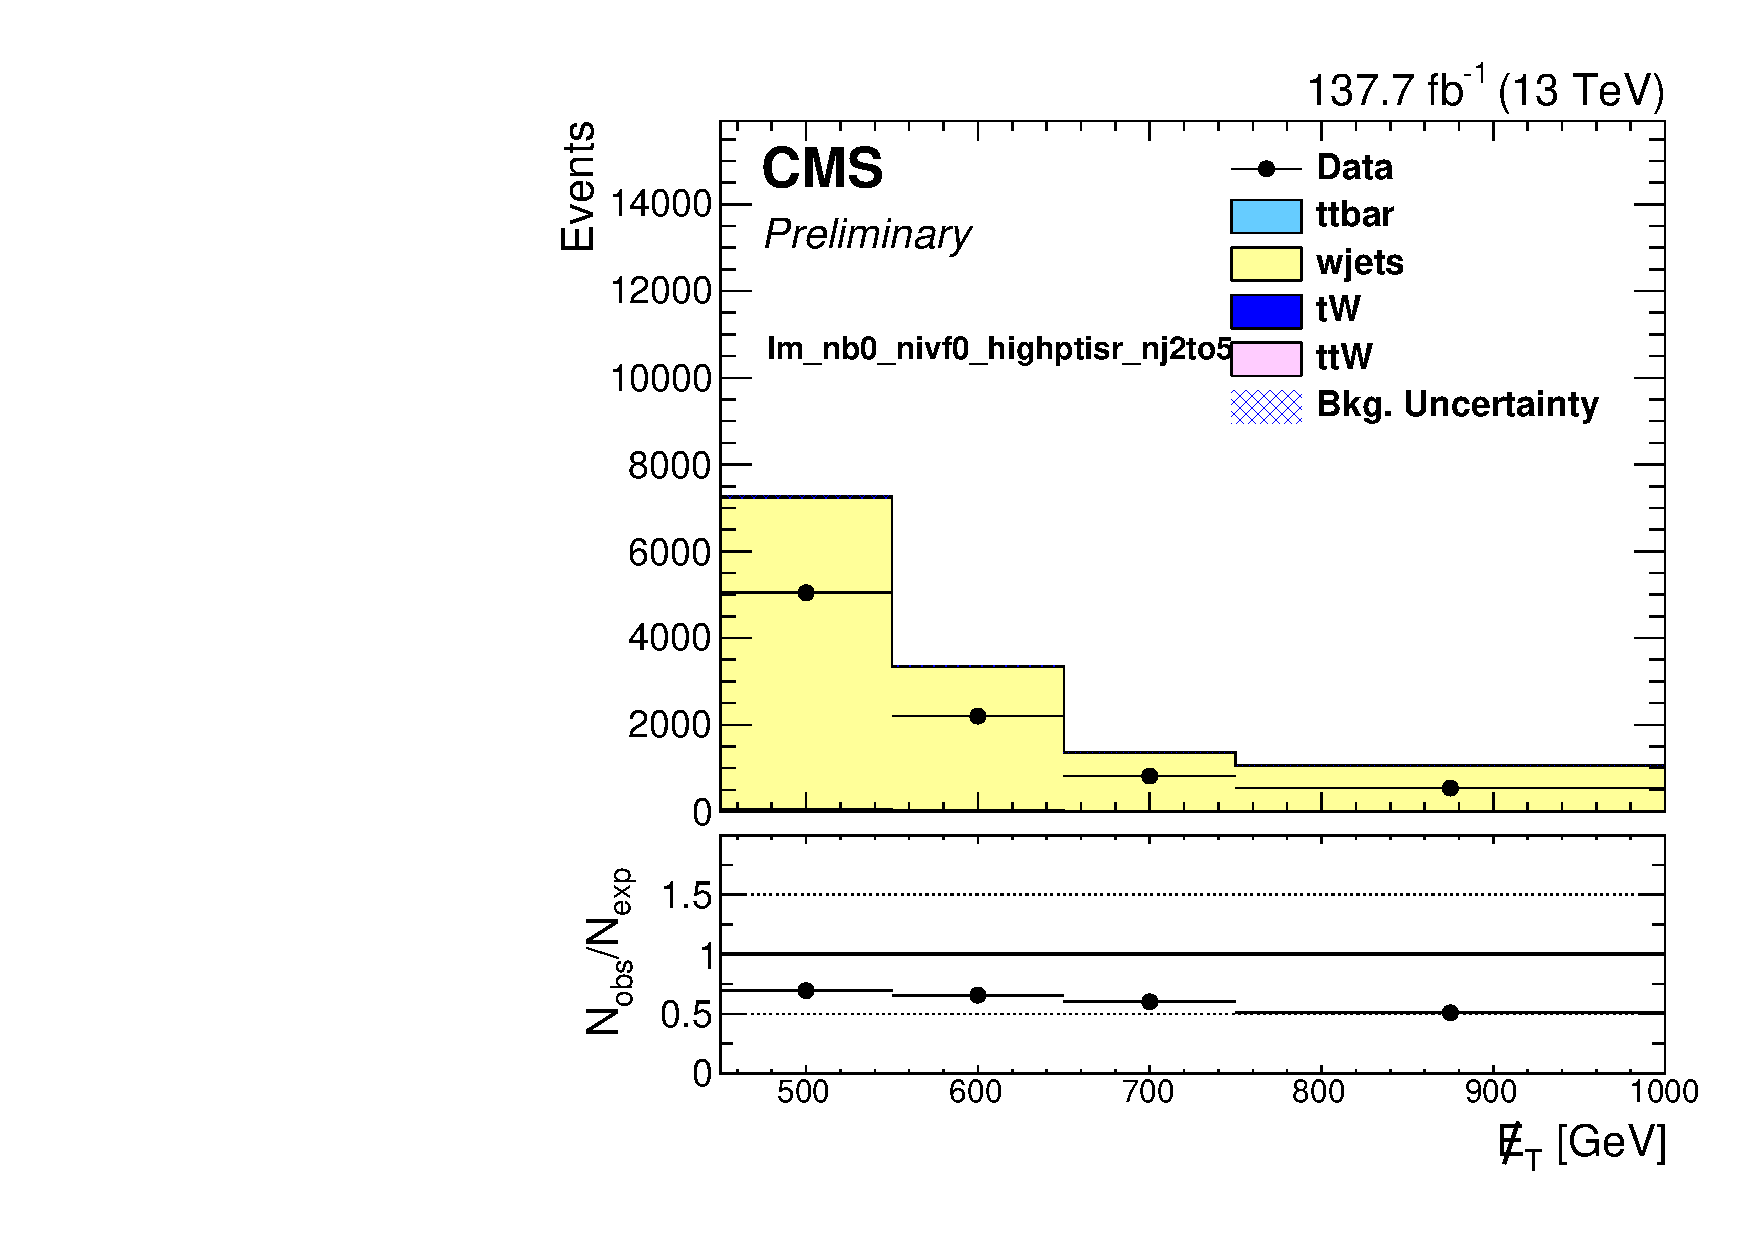
\includegraphics[width=0.49\textwidth]{lepcr_allEras/MET_pt_DataMC_lm_nb0_nivf0_highptisr_nj2to5__.pdf}
  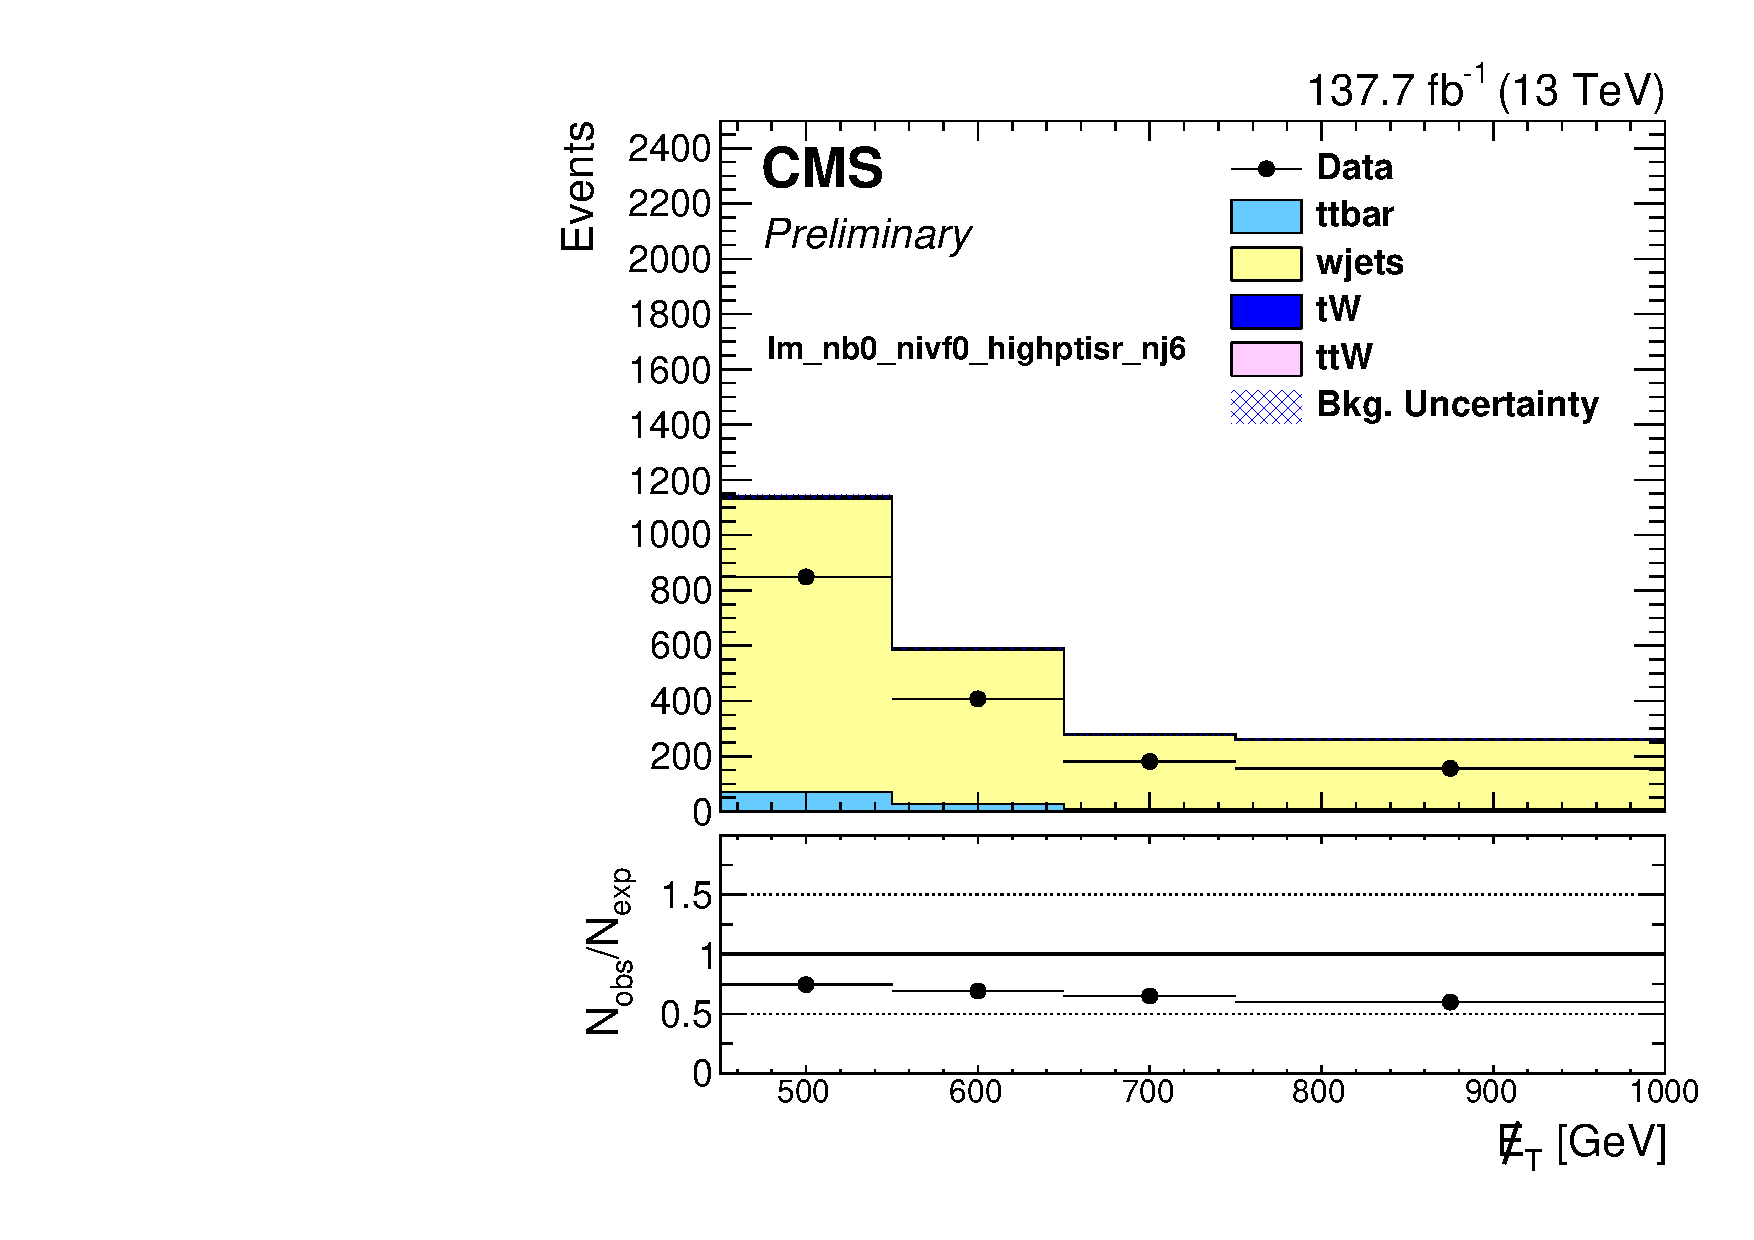
\includegraphics[width=0.49\textwidth]{lepcr_allEras/MET_pt_DataMC_lm_nb0_nivf0_highptisr_nj6__.pdf} \\
  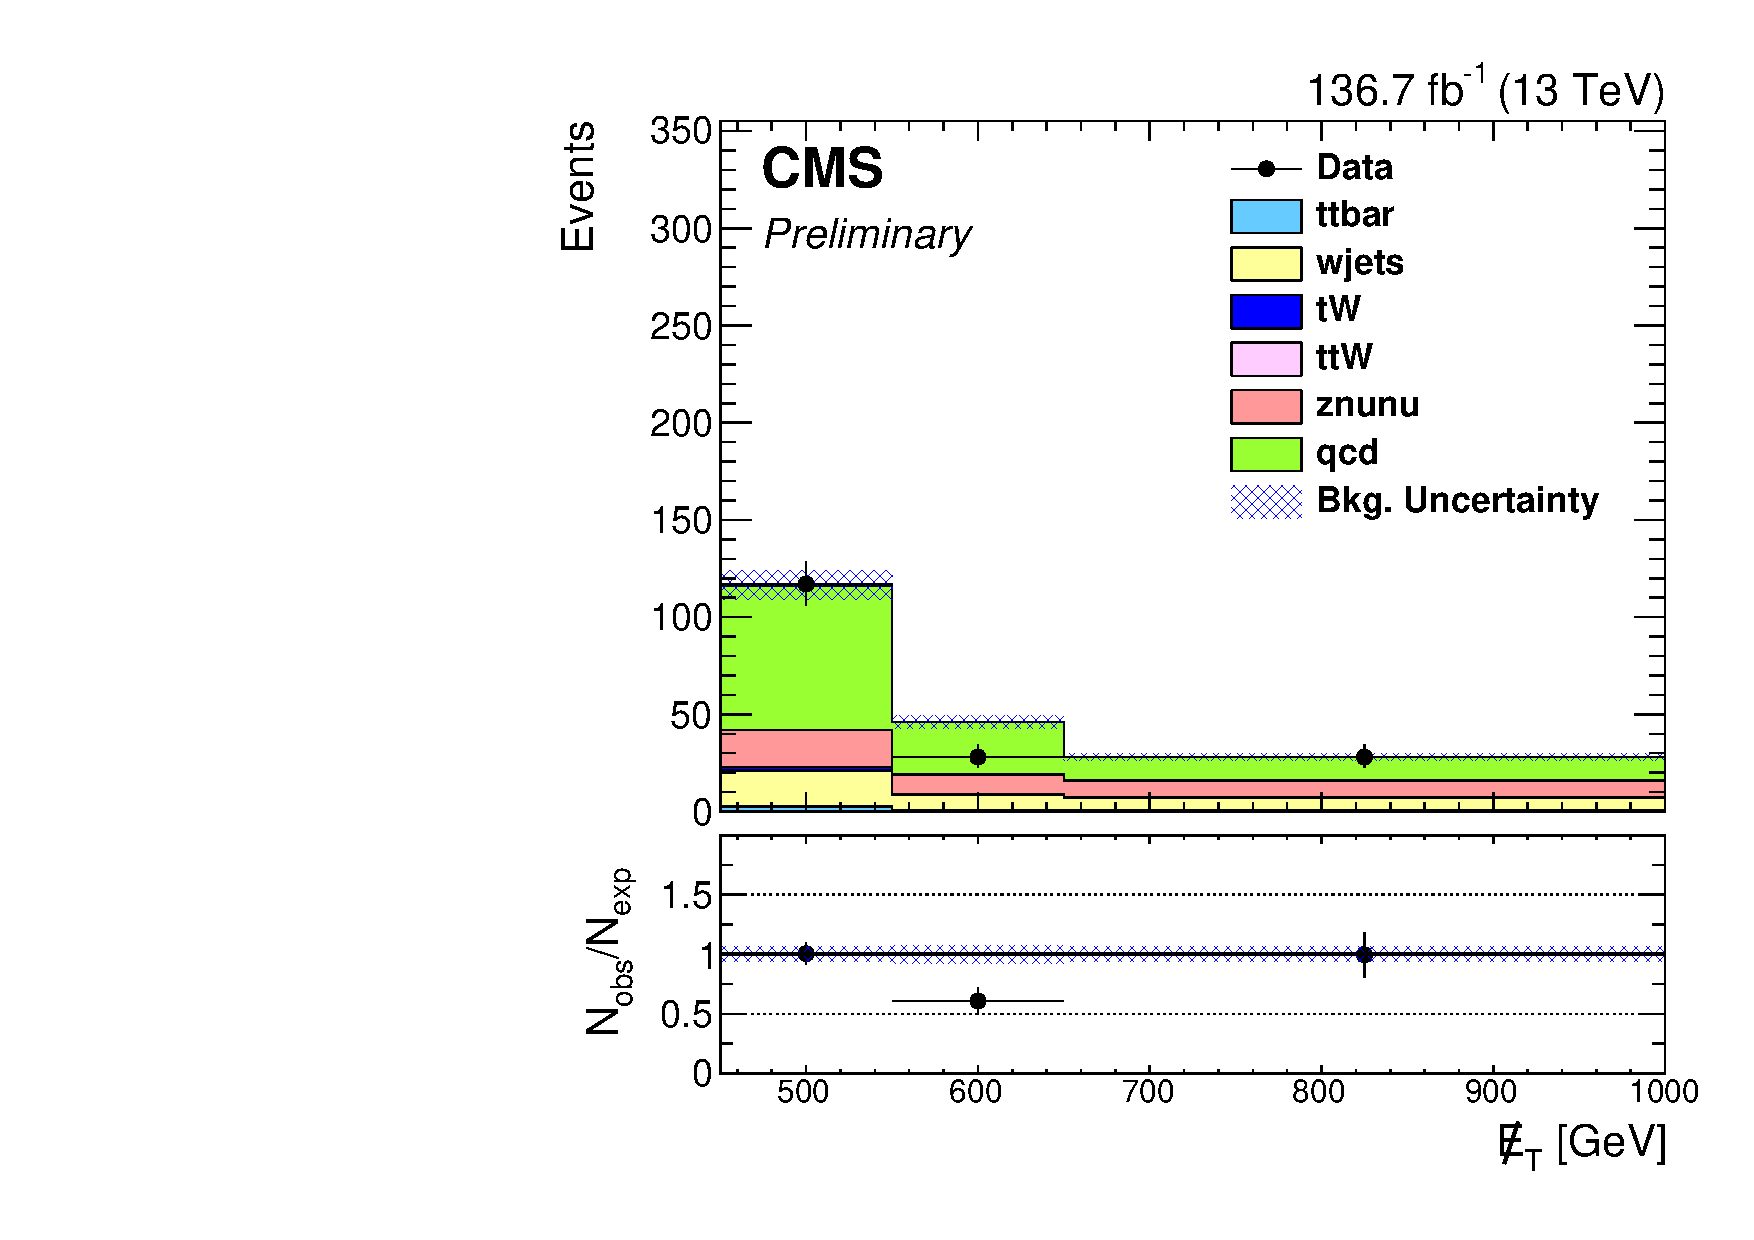
\includegraphics[width=0.49\textwidth]{lepcr_allEras/MET_pt_DataMC_lm_nb0_nivf1_highptisr_nj2to5__.pdf}
  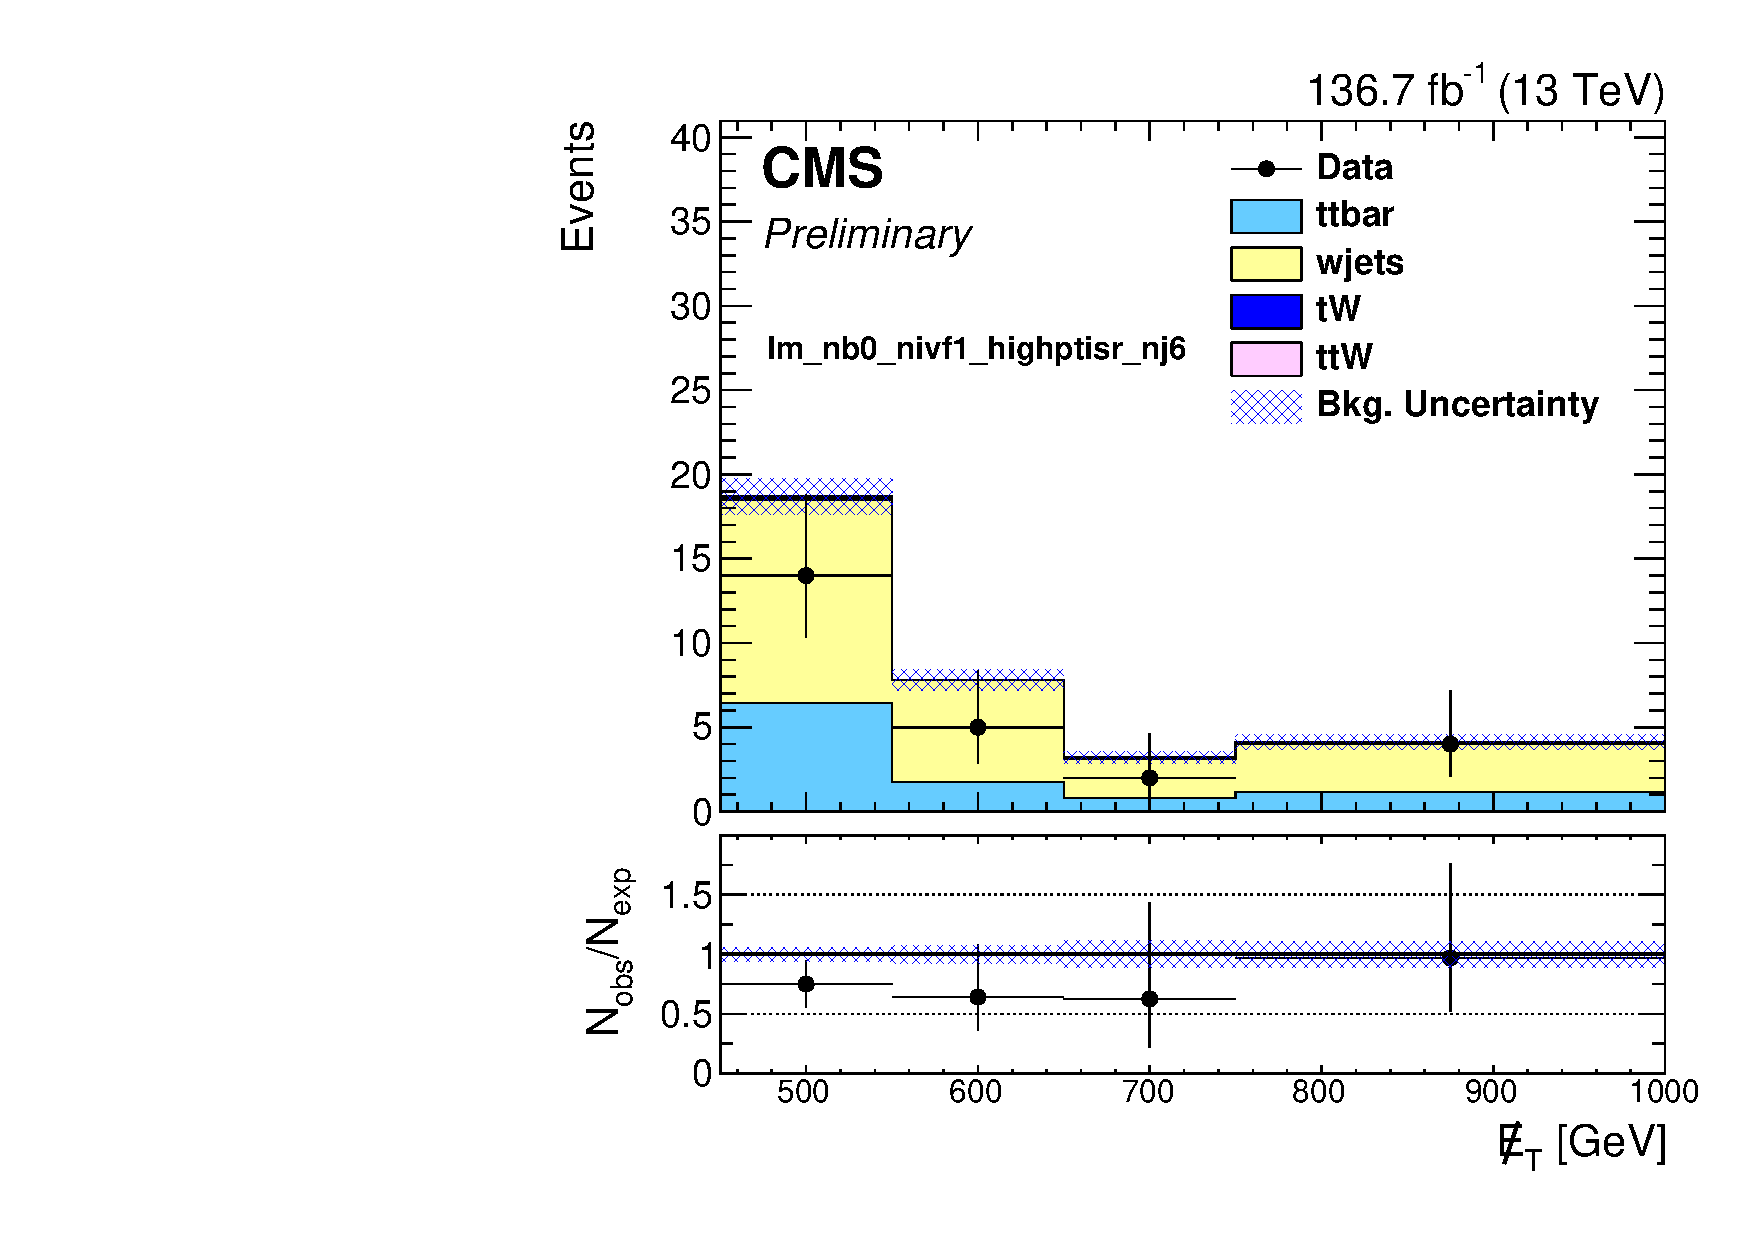
\includegraphics[width=0.49\textwidth]{lepcr_allEras/MET_pt_DataMC_lm_nb0_nivf1_highptisr_nj6__.pdf} \\
	\end{center}
	\caption[Lost Lepton LM Control Region $\nb=0$]{Comparison of the \met~distribution in the single-lepton sample after applying the low \dm~baseline selection in the $\nb=0$ region. Data and simulation are represented by the black points and stacked histograms, respectively. The error bars on the ratio of observed data to simulation correspond to the data statistical uncertainty and the shaded blue band represents the statistical uncertainty on the simulation. These regions are included with the search regions in the simultaneous fit for the signal extraction in order to estimate the LL contribution.
	 }
	\label{fig:llb-1lcr-datavsmc-lm-nb0}
\end{figure}
\begin{figure}[!h]
	\begin{center}  
		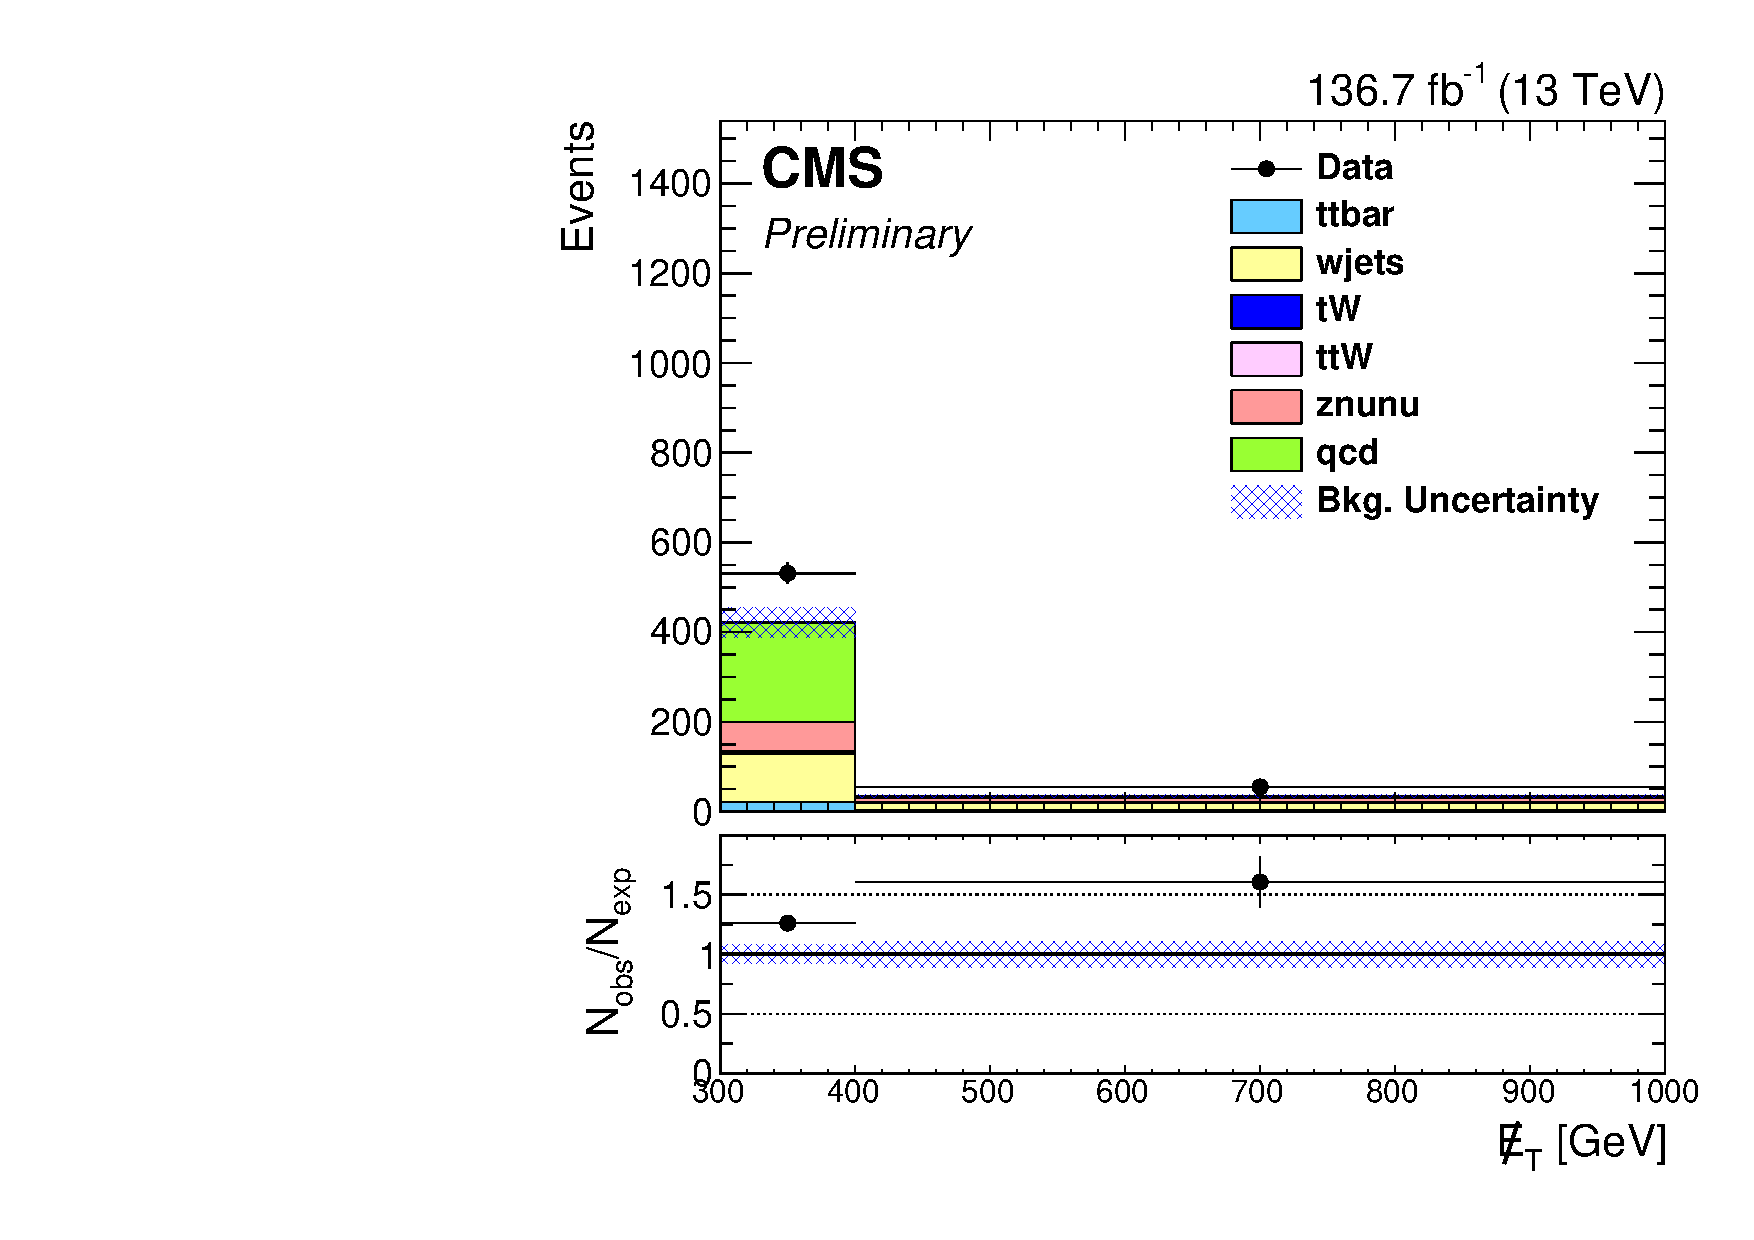
\includegraphics[width=0.32\textwidth]{lepcr_allEras/MET_pt_DataMC_lm_nb1_nivf0_lowmtb_lowptisr_lowptb__.pdf}
		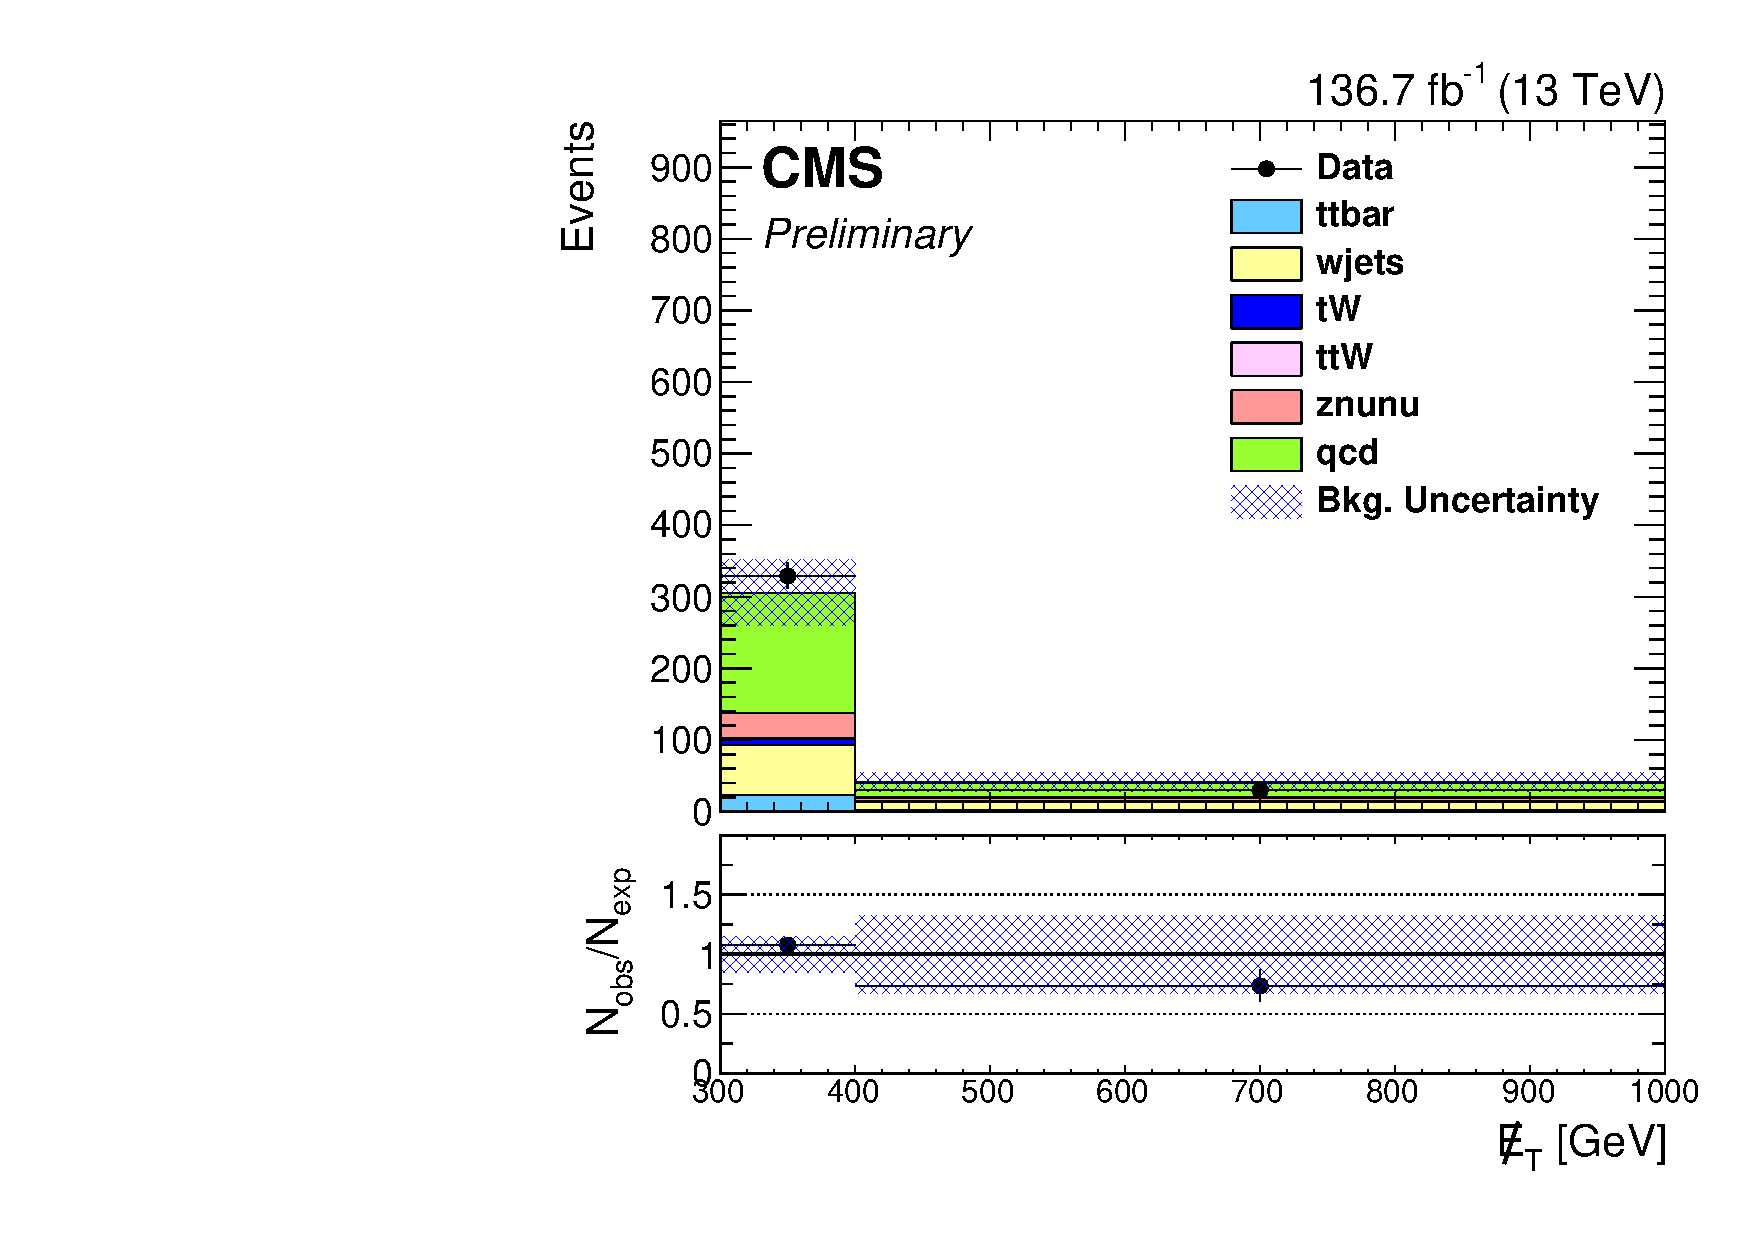
\includegraphics[width=0.32\textwidth]{lepcr_allEras/MET_pt_DataMC_lm_nb1_nivf0_lowmtb_lowptisr_medptb__.pdf} \\
		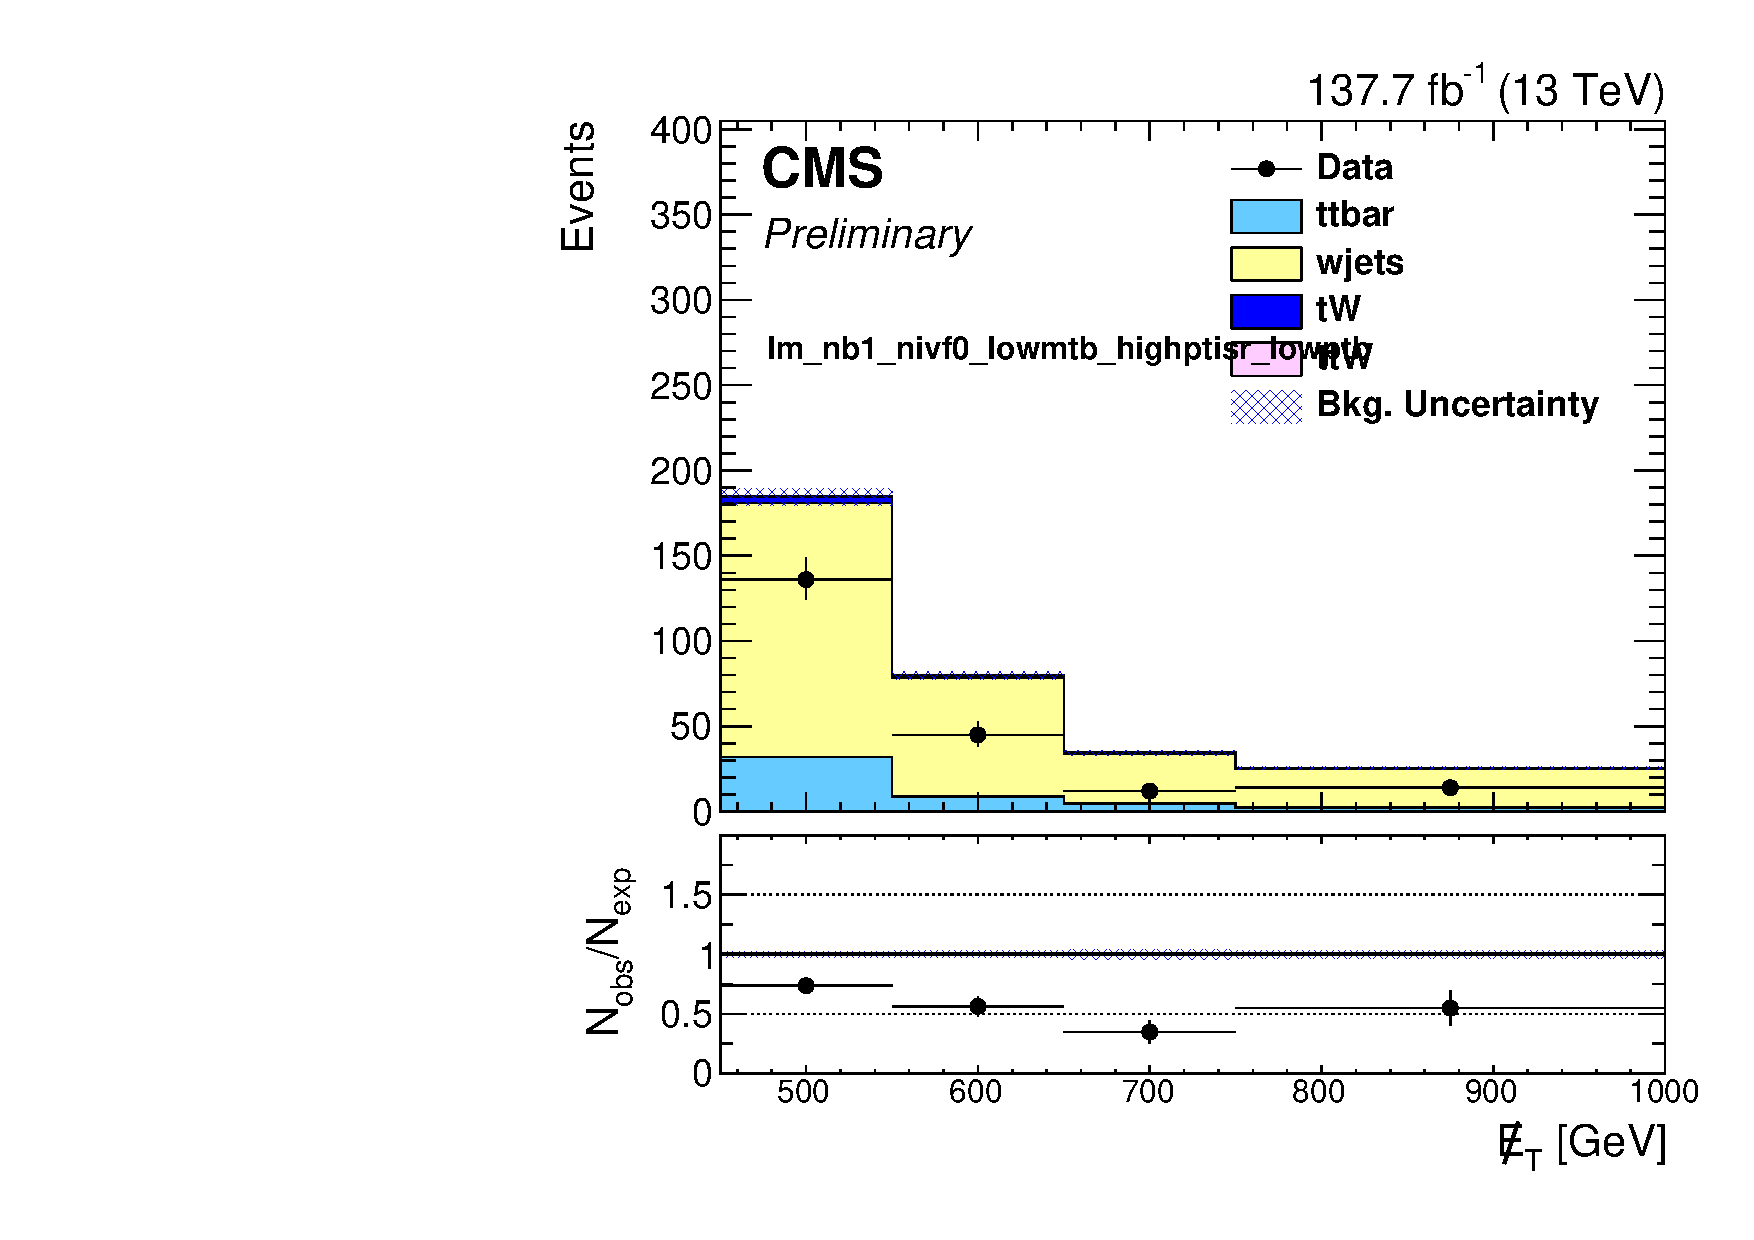
\includegraphics[width=0.32\textwidth]{lepcr_allEras/MET_pt_DataMC_lm_nb1_nivf0_lowmtb_highptisr_lowptb__.pdf}
		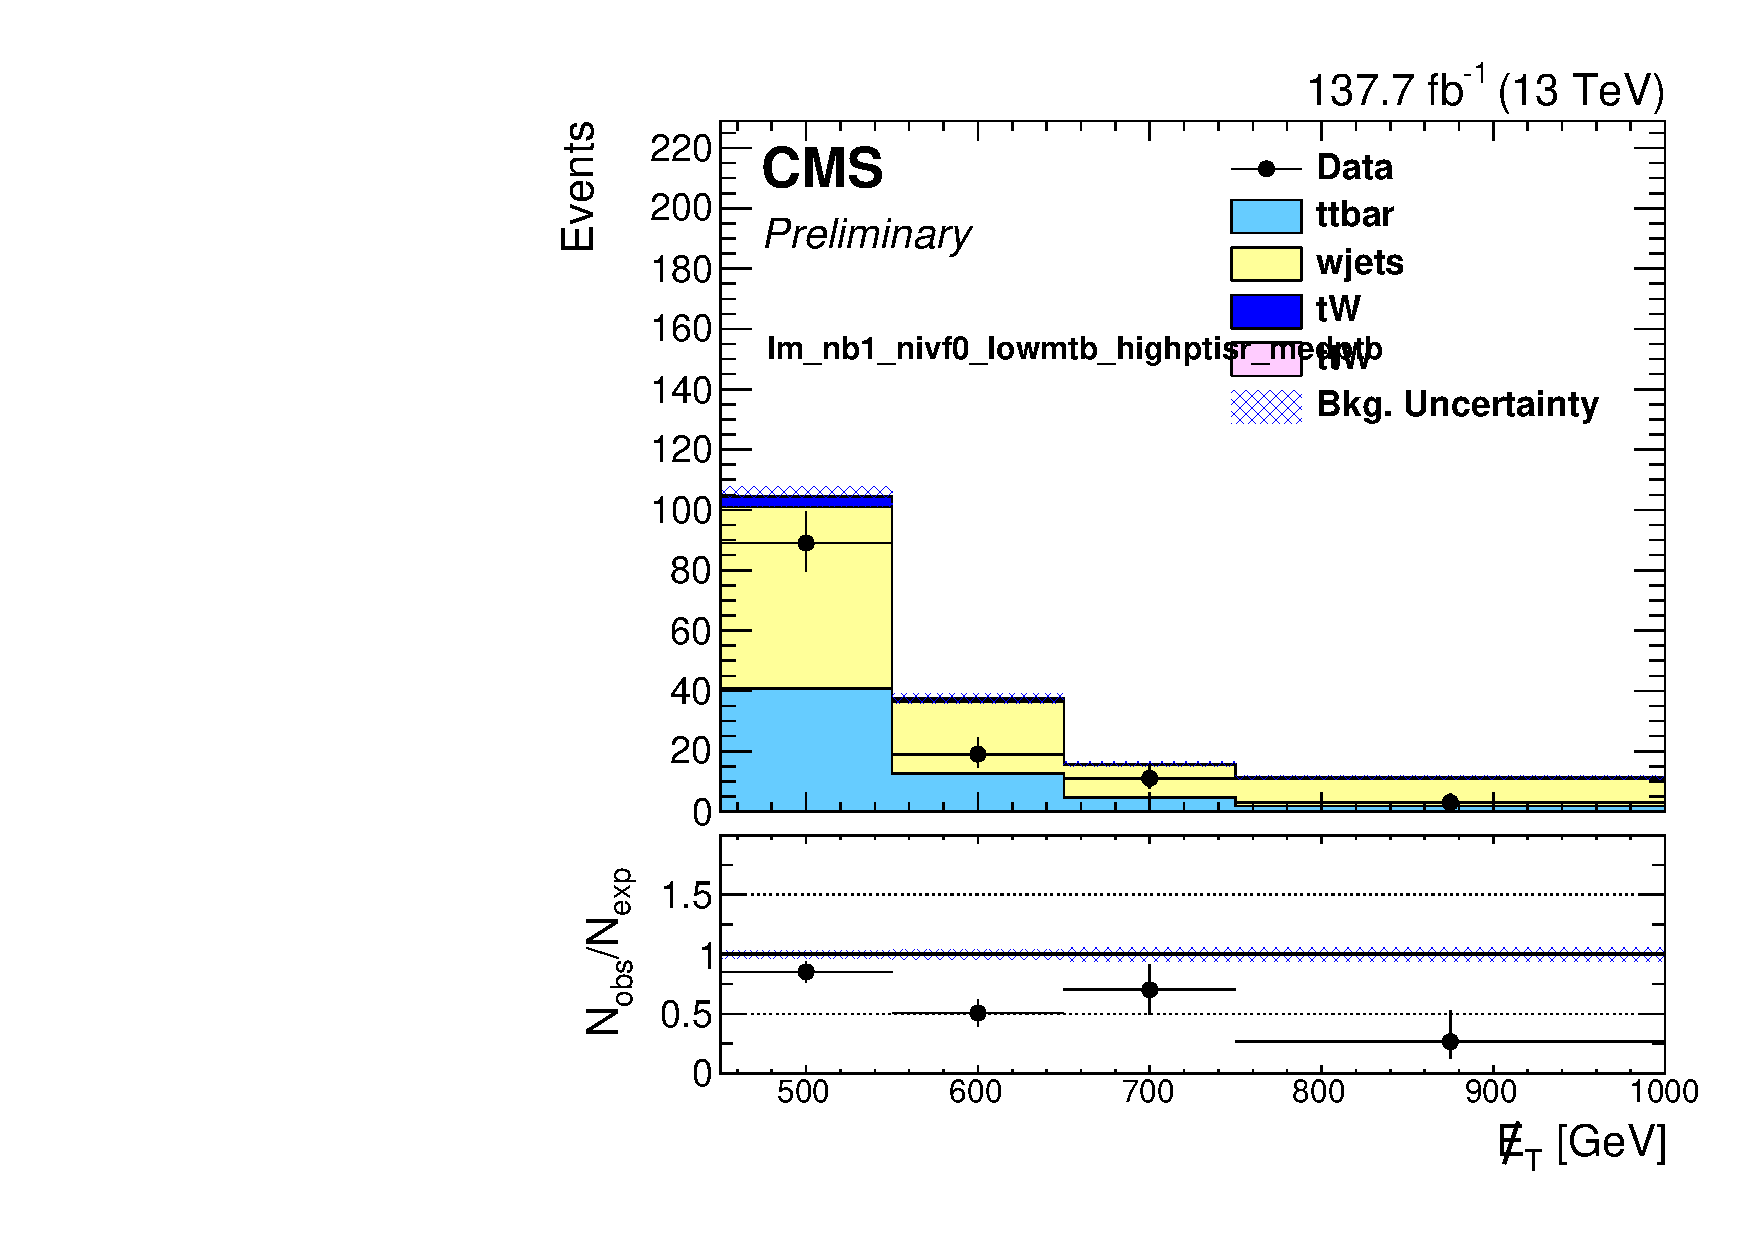
\includegraphics[width=0.32\textwidth]{lepcr_allEras/MET_pt_DataMC_lm_nb1_nivf0_lowmtb_highptisr_medptb__.pdf}
		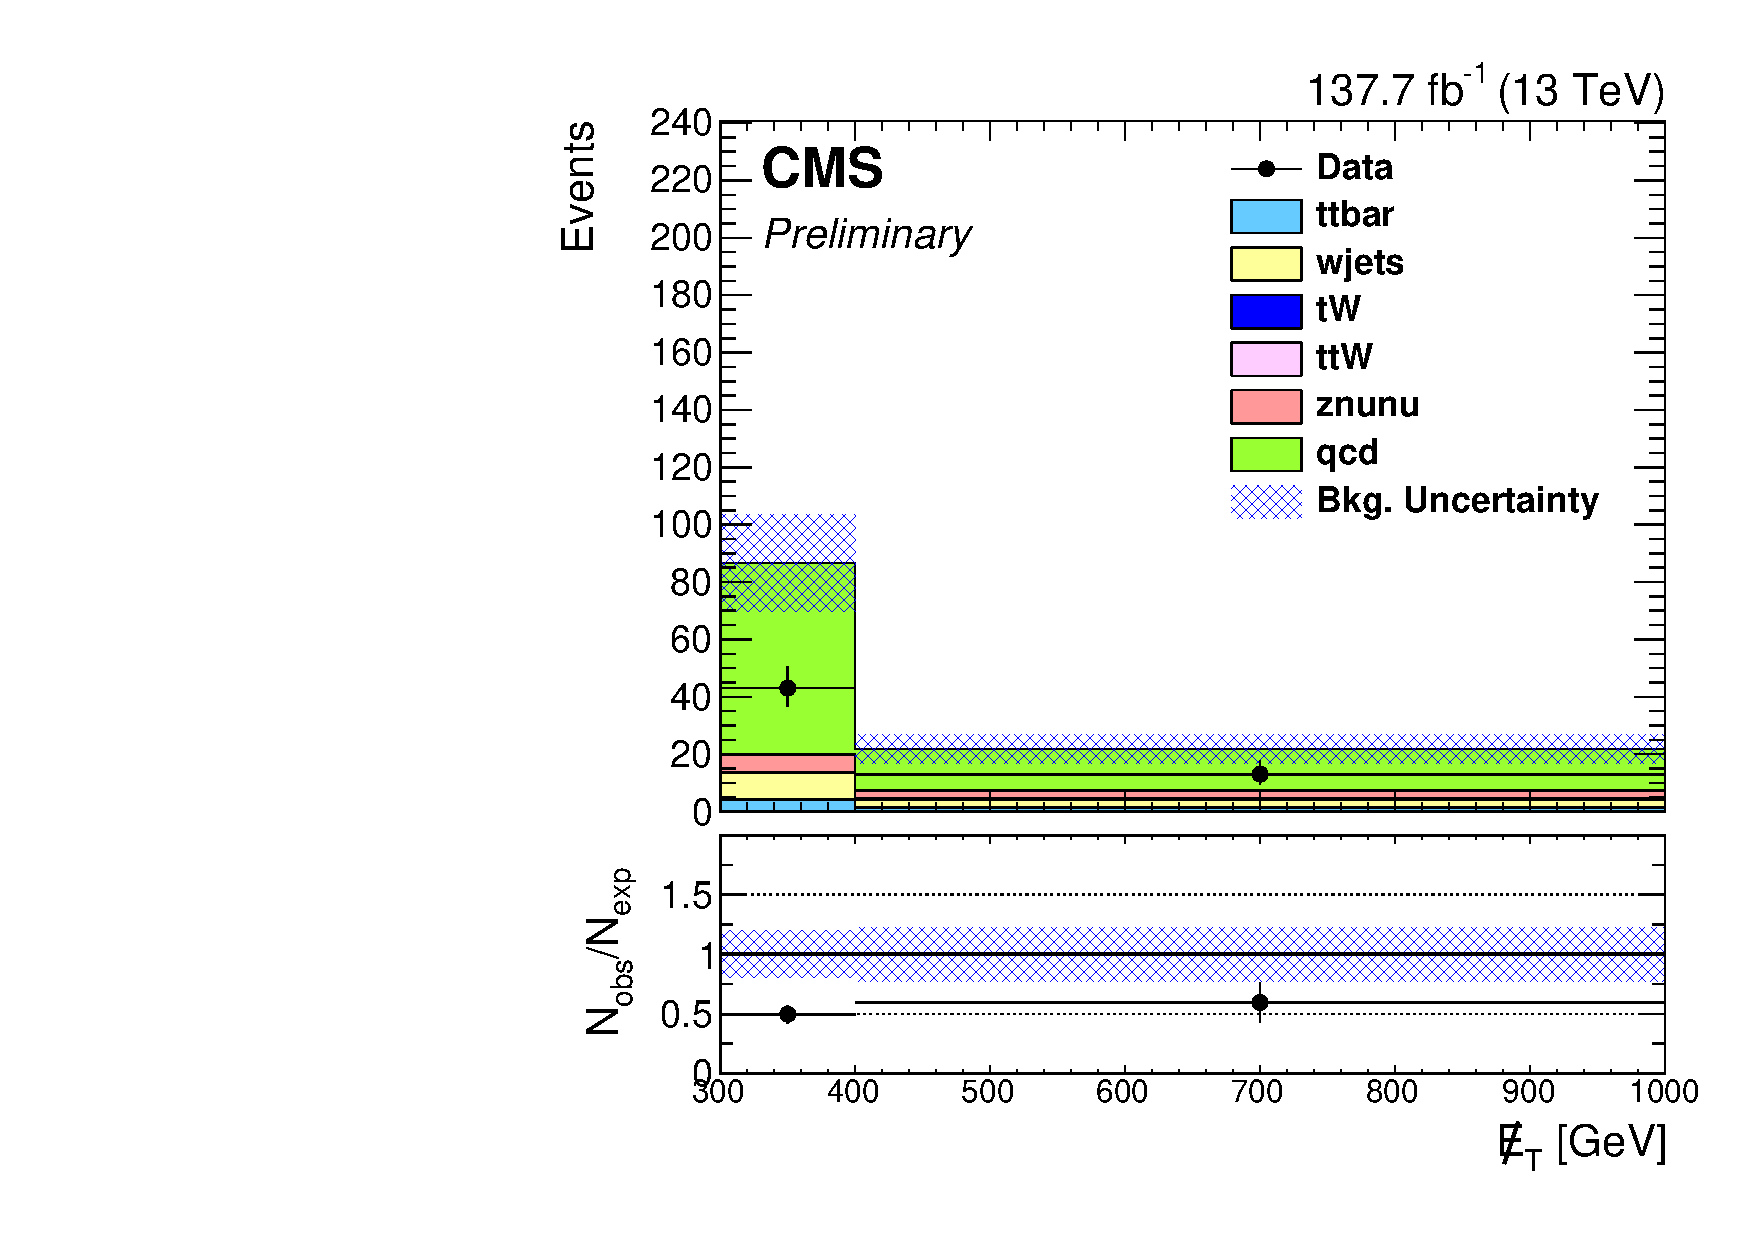
\includegraphics[width=0.32\textwidth]{lepcr_allEras/MET_pt_DataMC_lm_nb1_nivf1_lowmtb_lowptb__.pdf} \\
		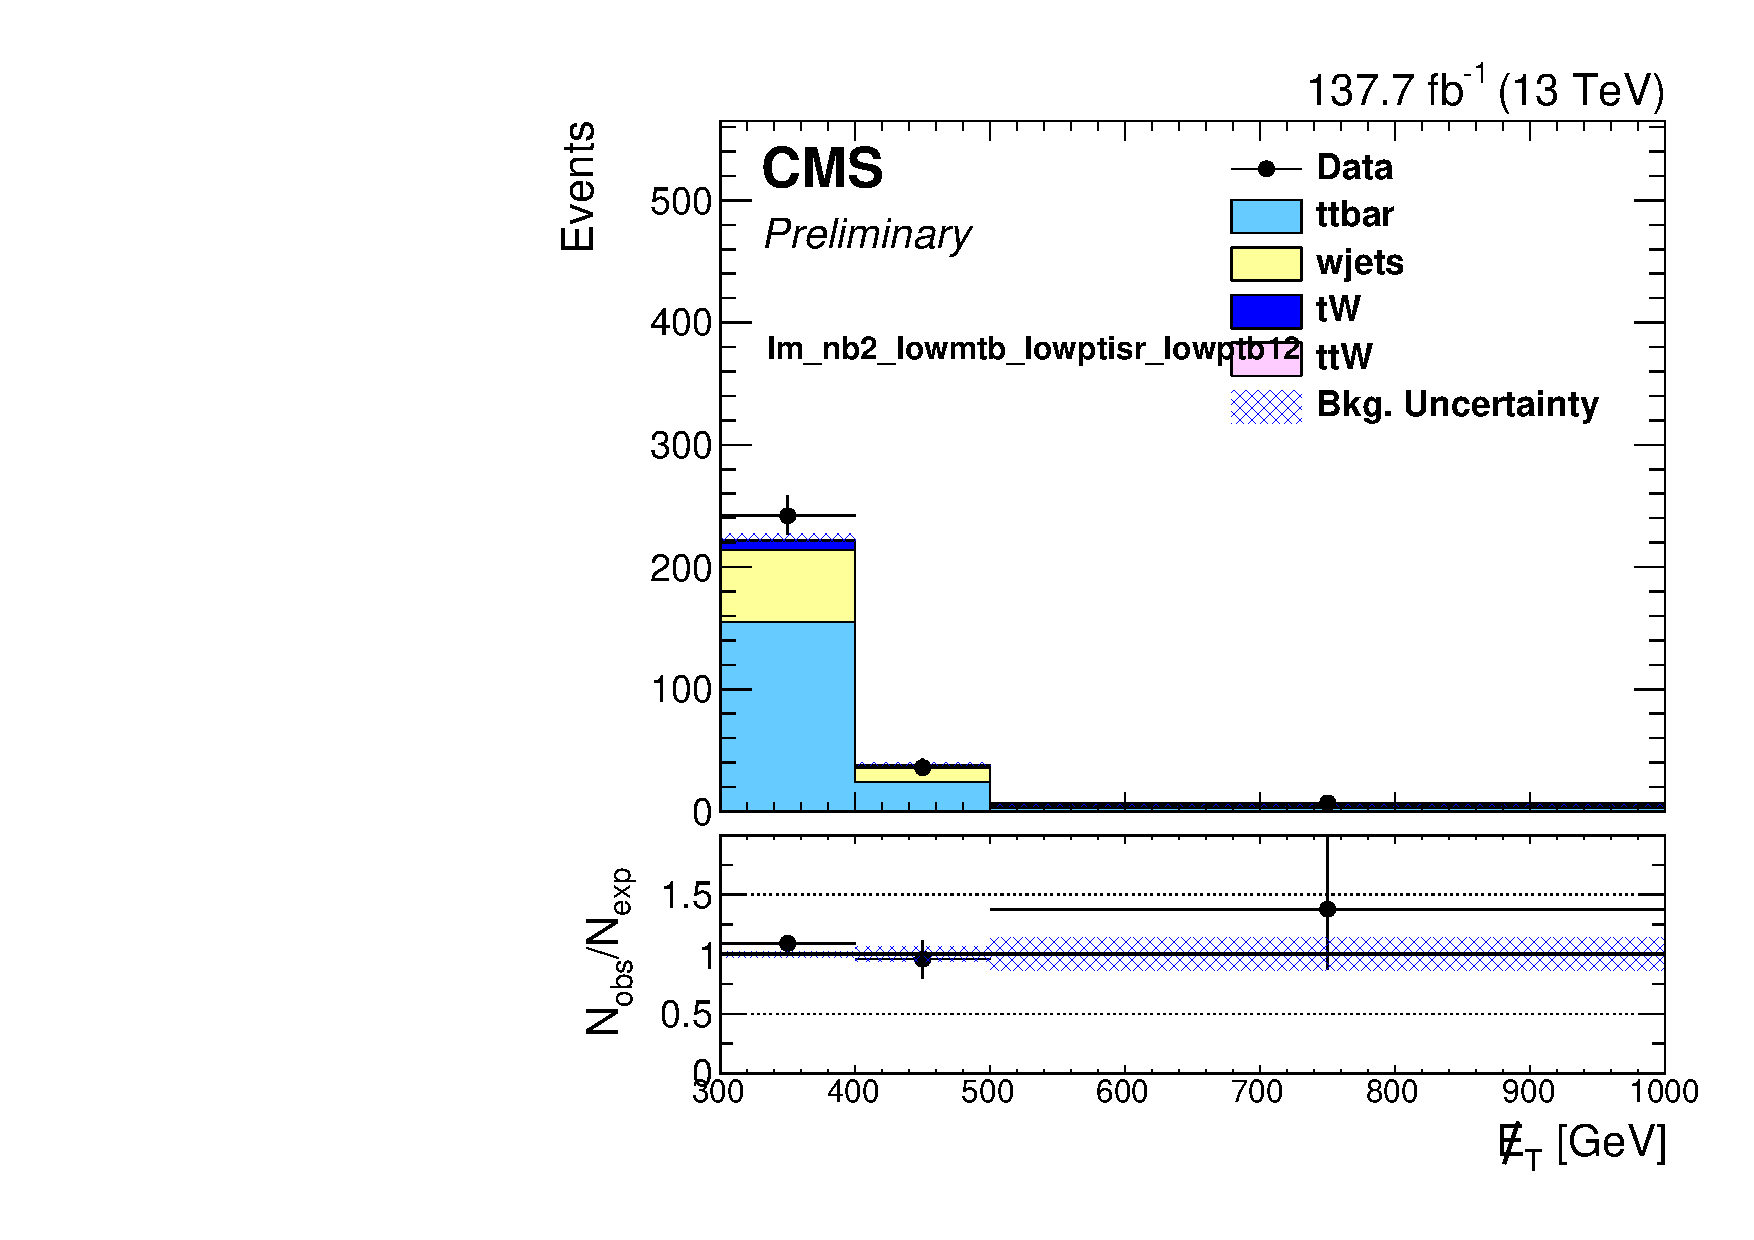
\includegraphics[width=0.32\textwidth]{lepcr_allEras/MET_pt_DataMC_lm_nb2_lowmtb_lowptisr_lowptb12__.pdf} 
		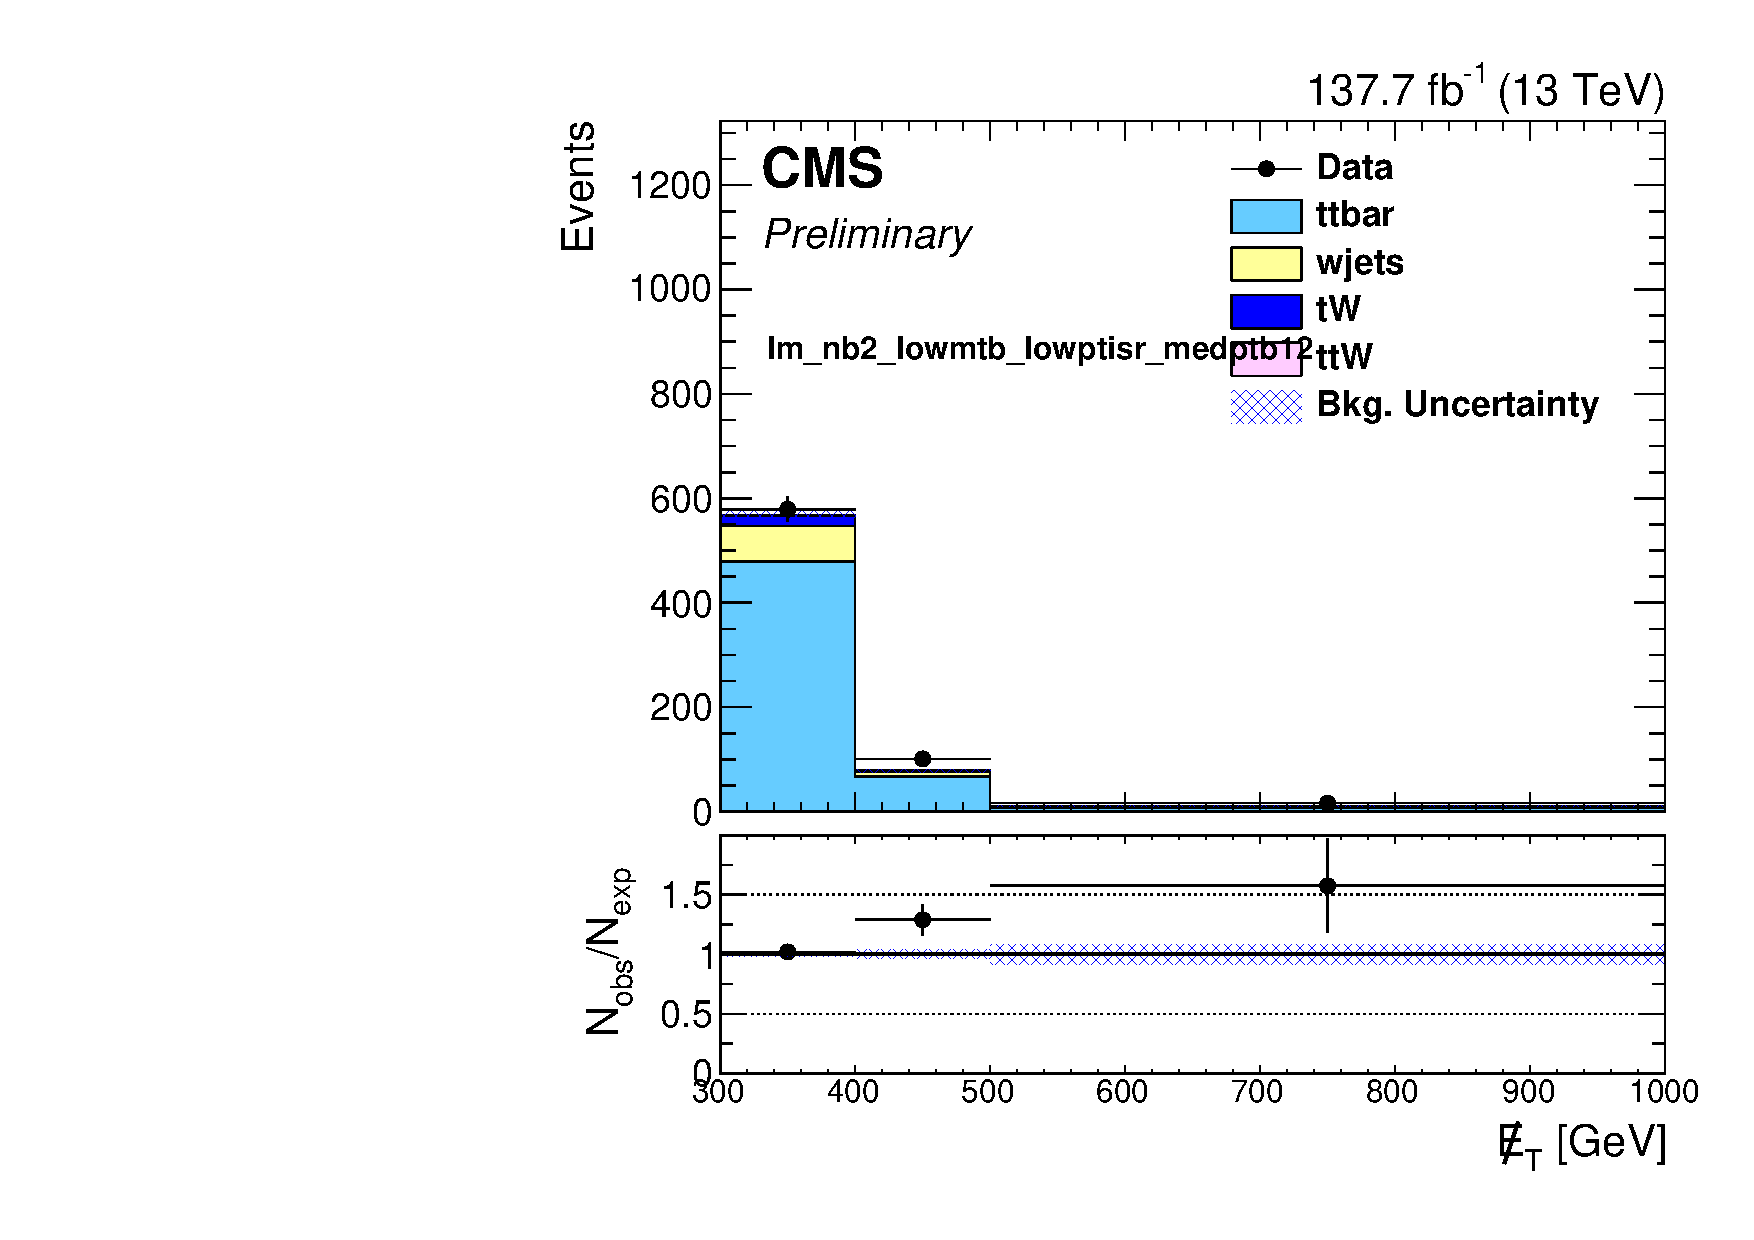
\includegraphics[width=0.32\textwidth]{lepcr_allEras/MET_pt_DataMC_lm_nb2_lowmtb_lowptisr_medptb12__.pdf}
		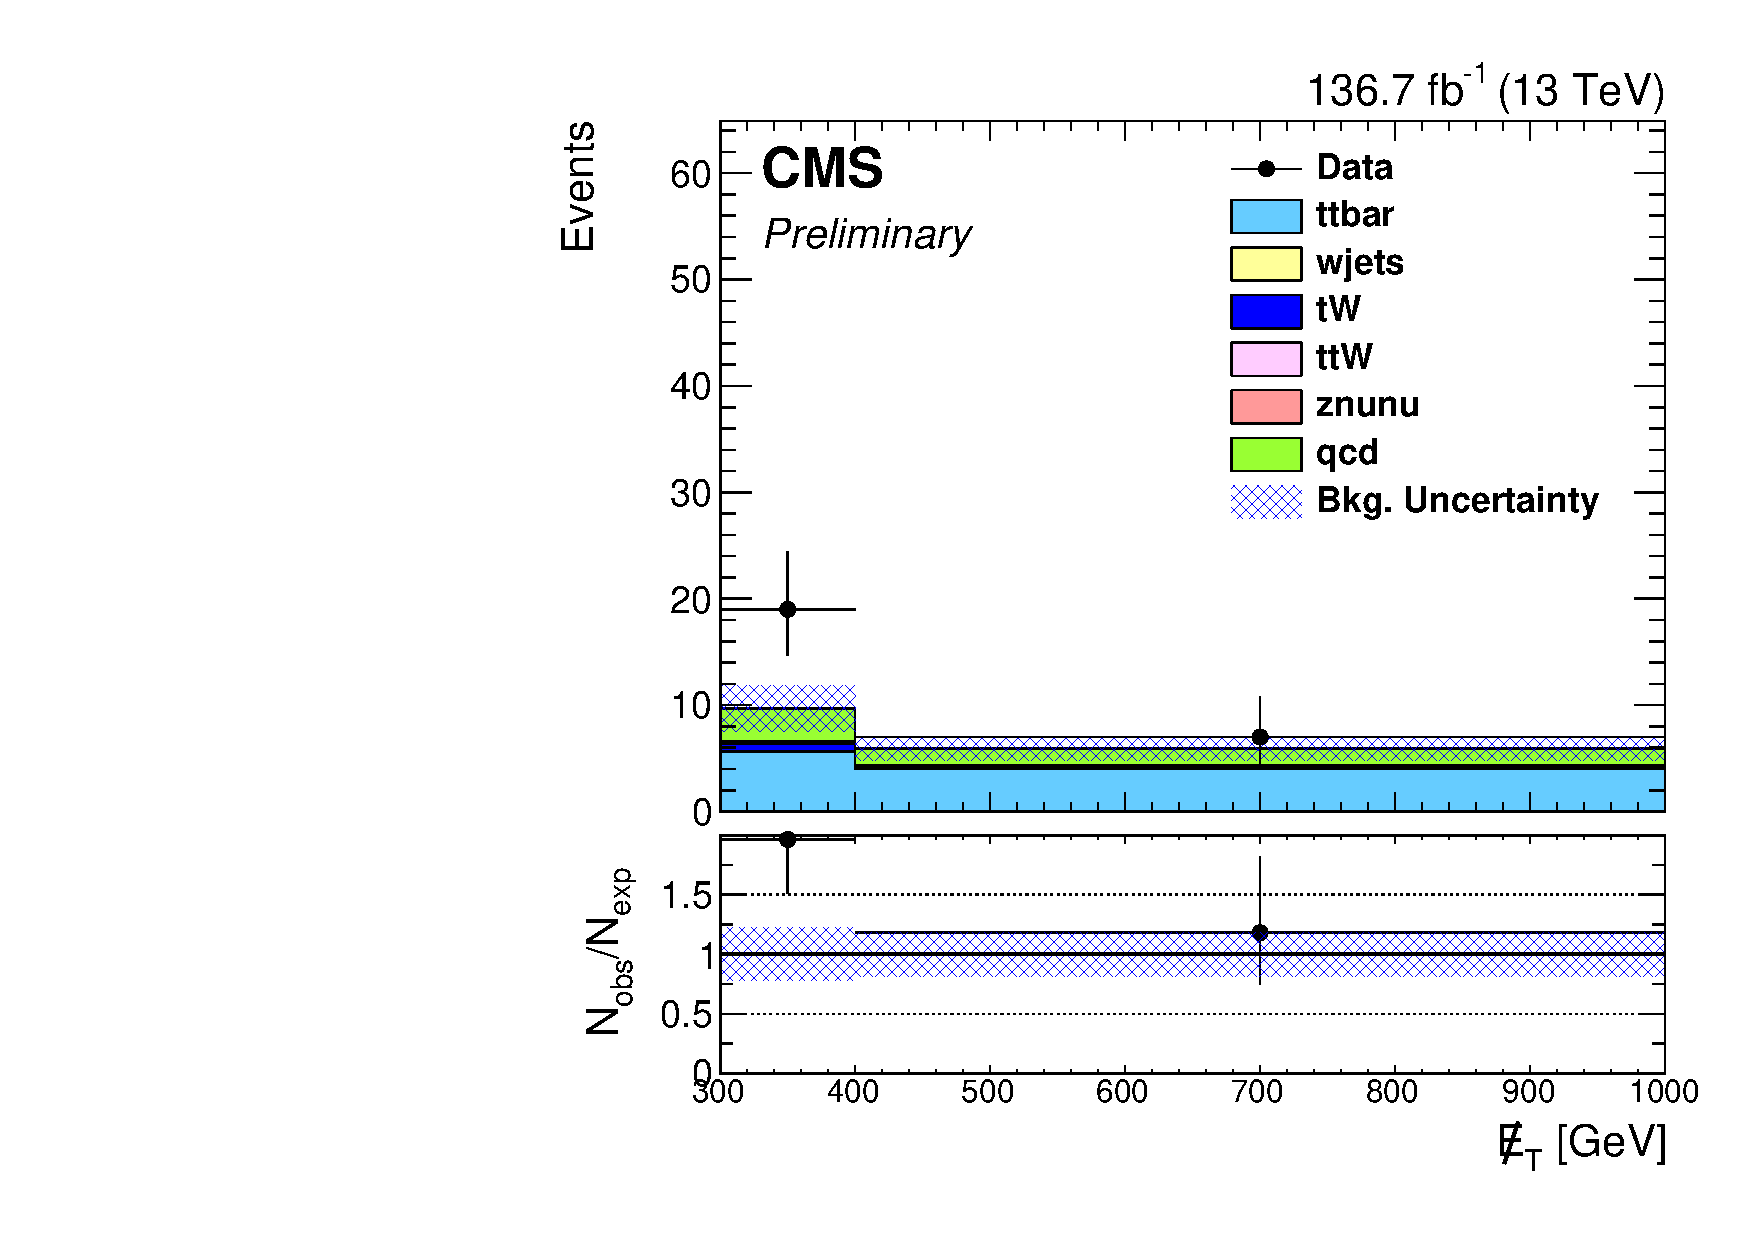
\includegraphics[width=0.32\textwidth]{lepcr_allEras/MET_pt_DataMC_lm_nb2_lowmtb_lowptisr_highptb12_nj7__.pdf} \\
		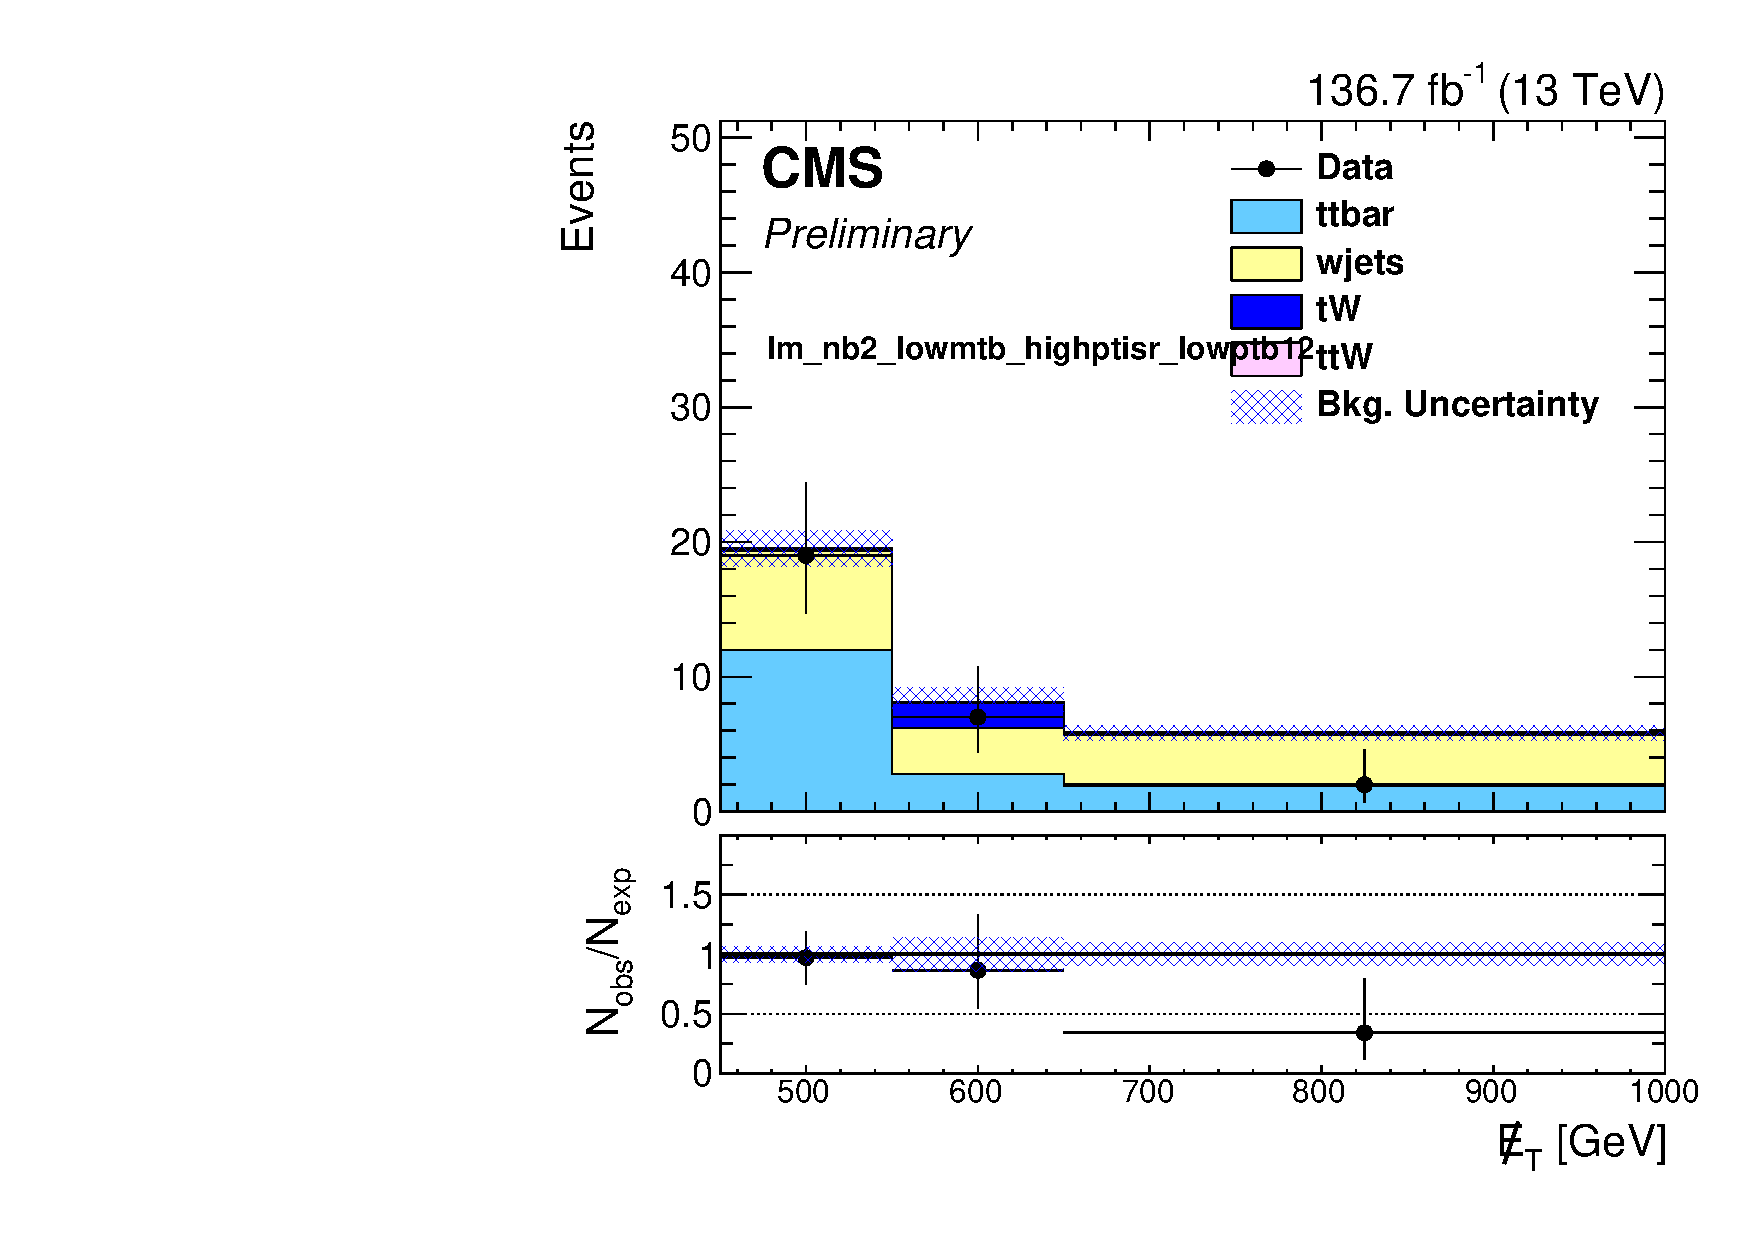
\includegraphics[width=0.32\textwidth]{lepcr_allEras/MET_pt_DataMC_lm_nb2_lowmtb_highptisr_lowptb12__.pdf} 
		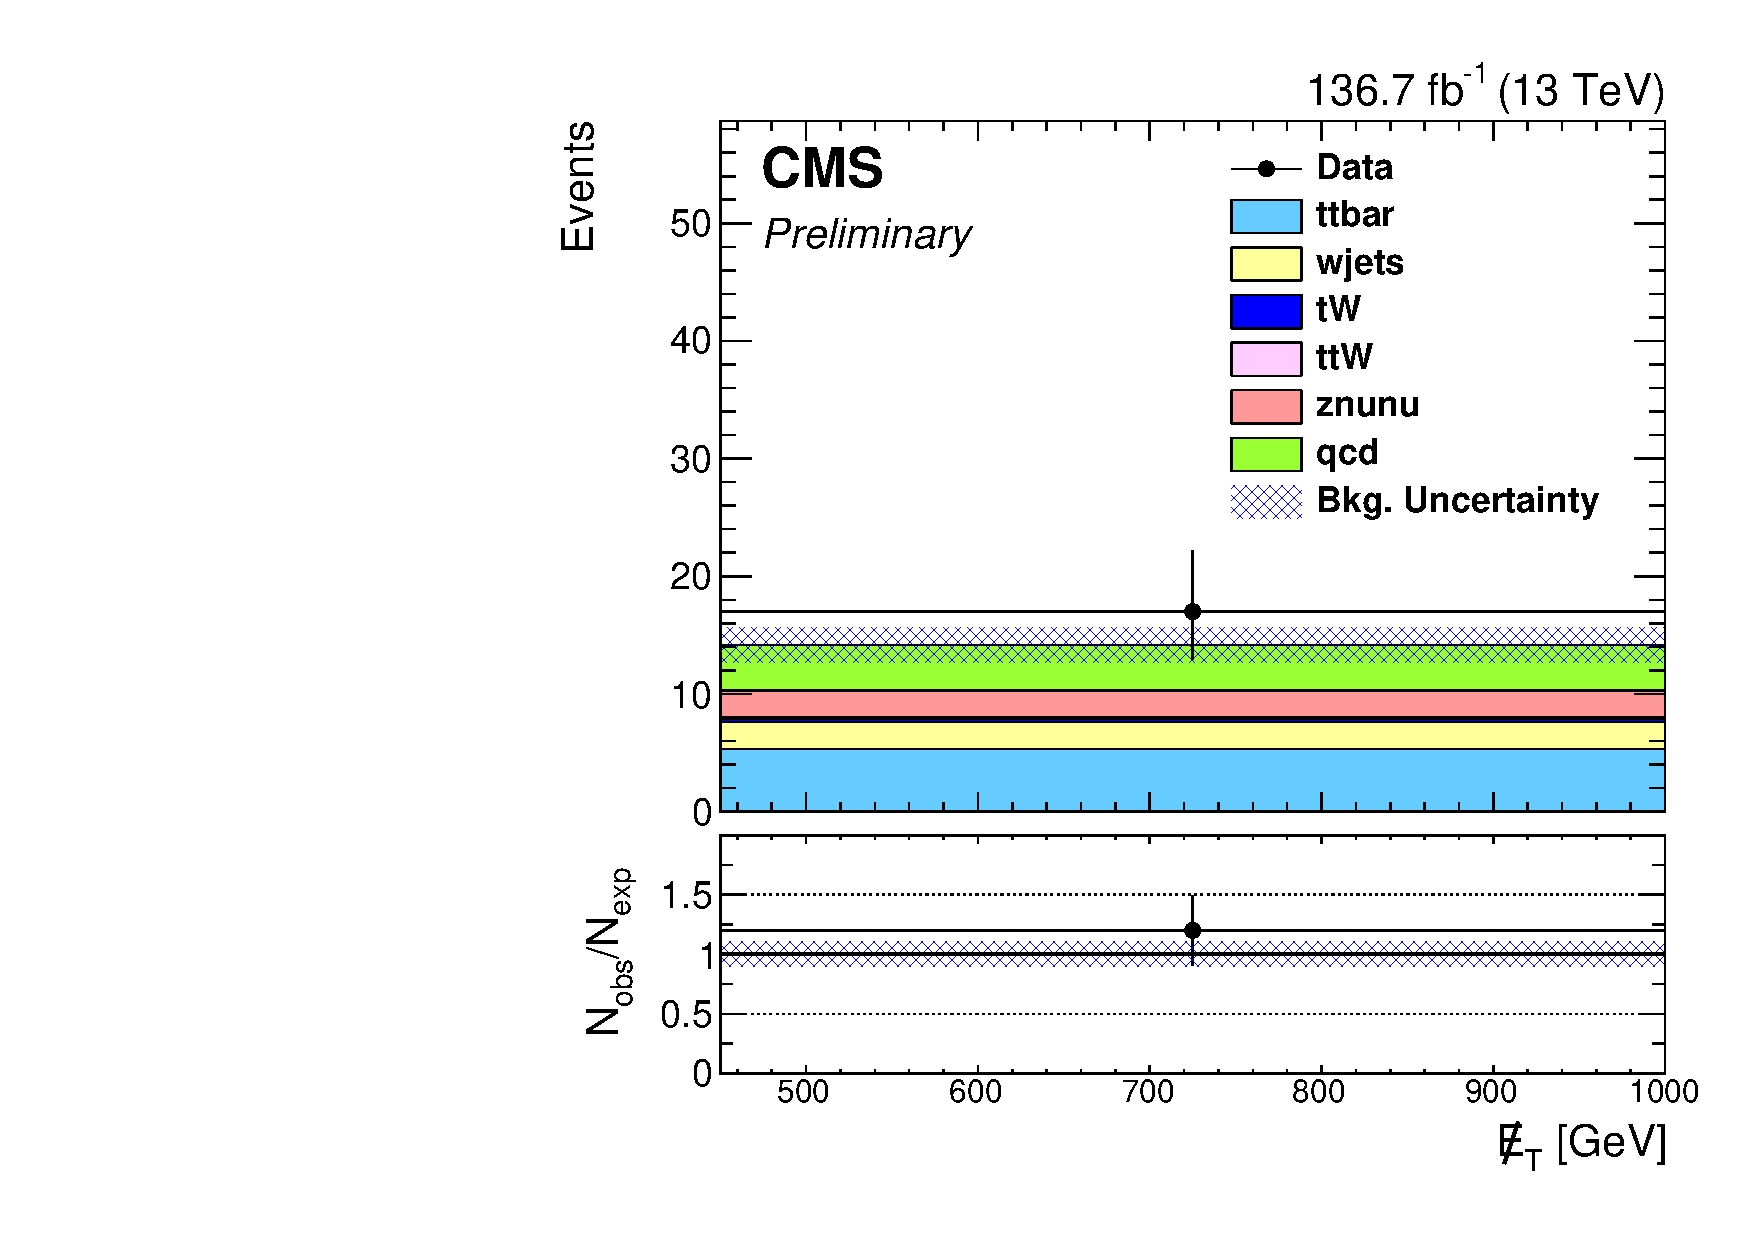
\includegraphics[width=0.32\textwidth]{lepcr_allEras/MET_pt_DataMC_lm_nb2_lowmtb_highptisr_medptb12__.pdf}
		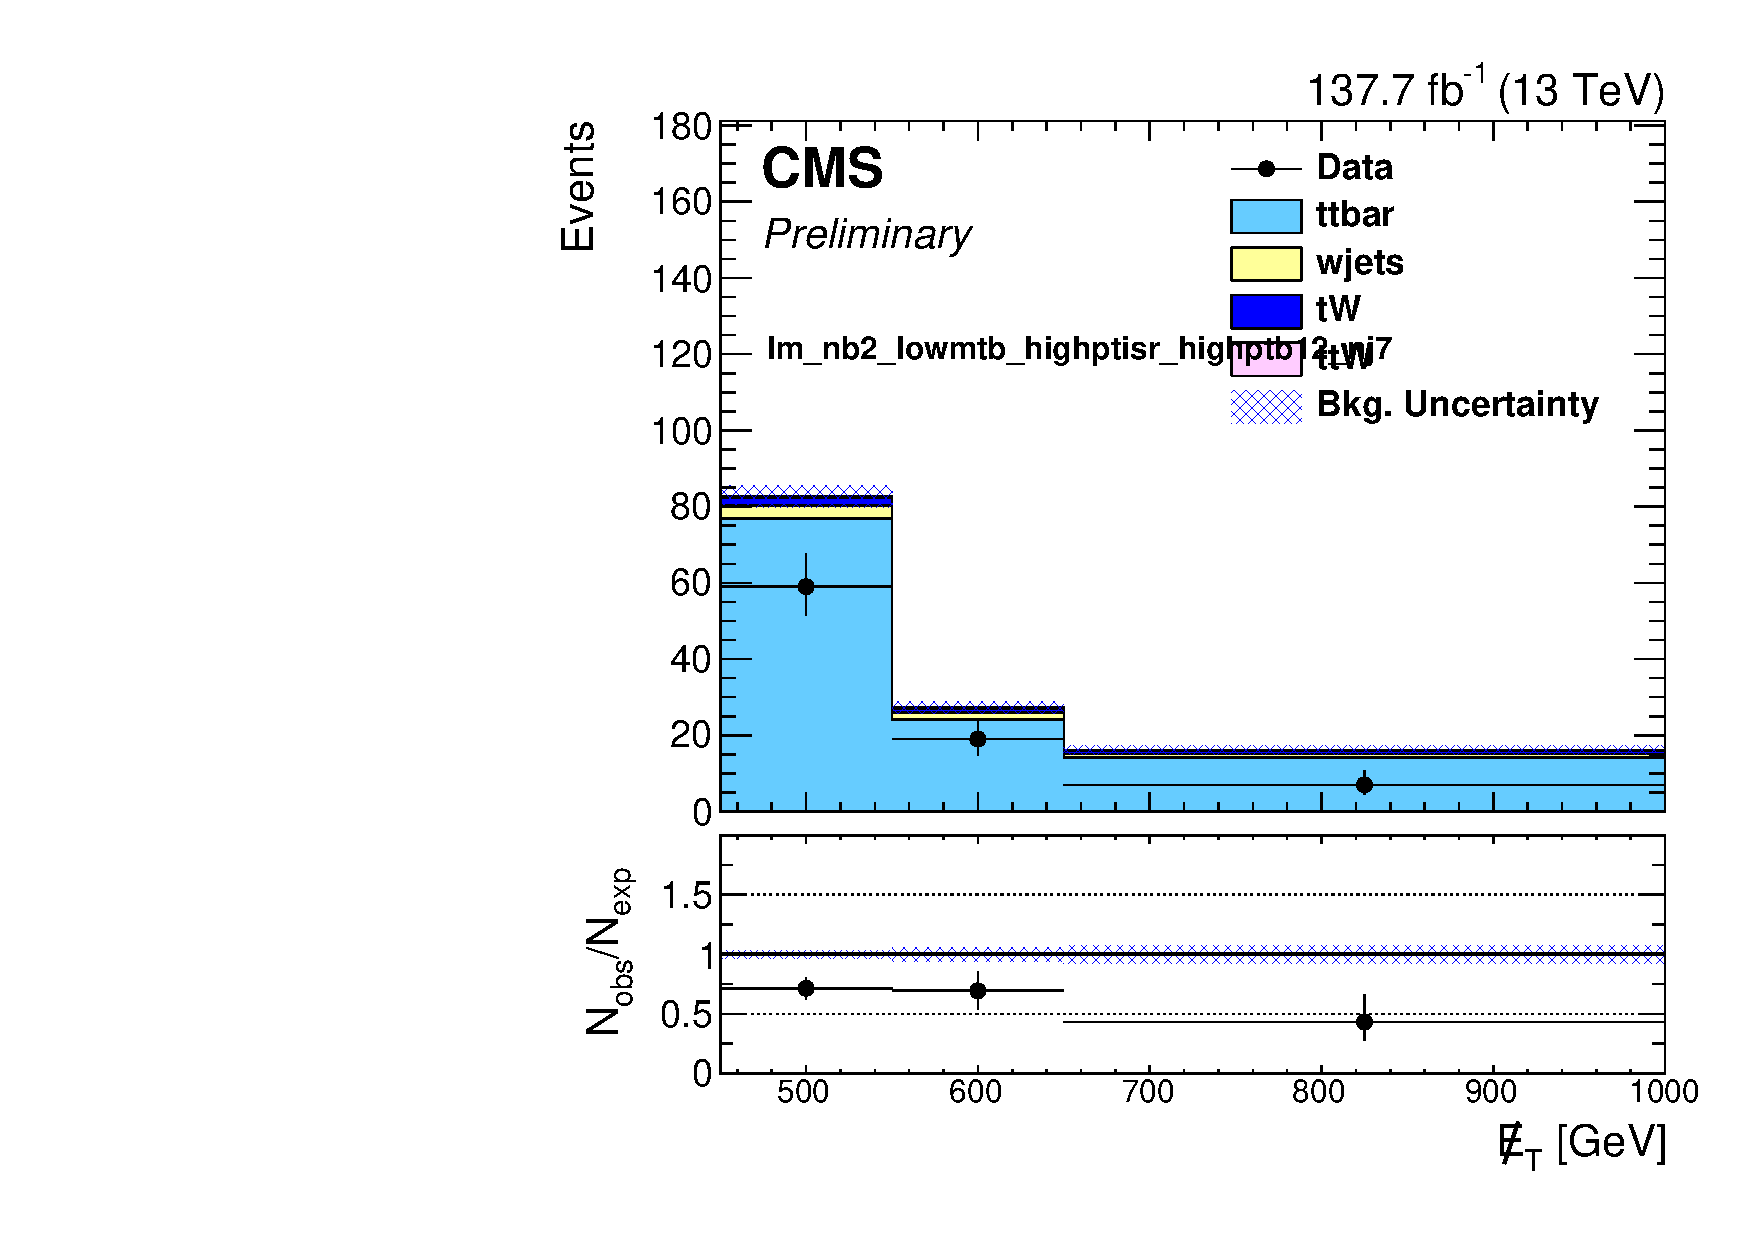
\includegraphics[width=0.32\textwidth]{lepcr_allEras/MET_pt_DataMC_lm_nb2_lowmtb_highptisr_highptb12_nj7__.pdf} \\
	\end{center}
	\caption[Lost Lepton LM Control Region $\nb=1$]{Comparison of the \met~distribution in the single-lepton sample after applying the low \dm~baseline selection. Two top rows: Events with $\nb=1$; Two bottom rows: Events with $\nb \geq2$;  Data and simulation are represented by the black points and stacked histograms, respectively. The error bars on the ratio of observed data to simulation correspond to the data statistical uncertainty and the shaded blue band represents the statistical uncertainty on the simulation. These regions are included with the search regions in the simultaneous fit for the signal extraction in order to estimate the LL contribution.
	 }
	\label{fig:llb-1lcr-datavsmc-lm-nb1}
\end{figure}

\begin{figure}[!htb]
	\begin{center}
  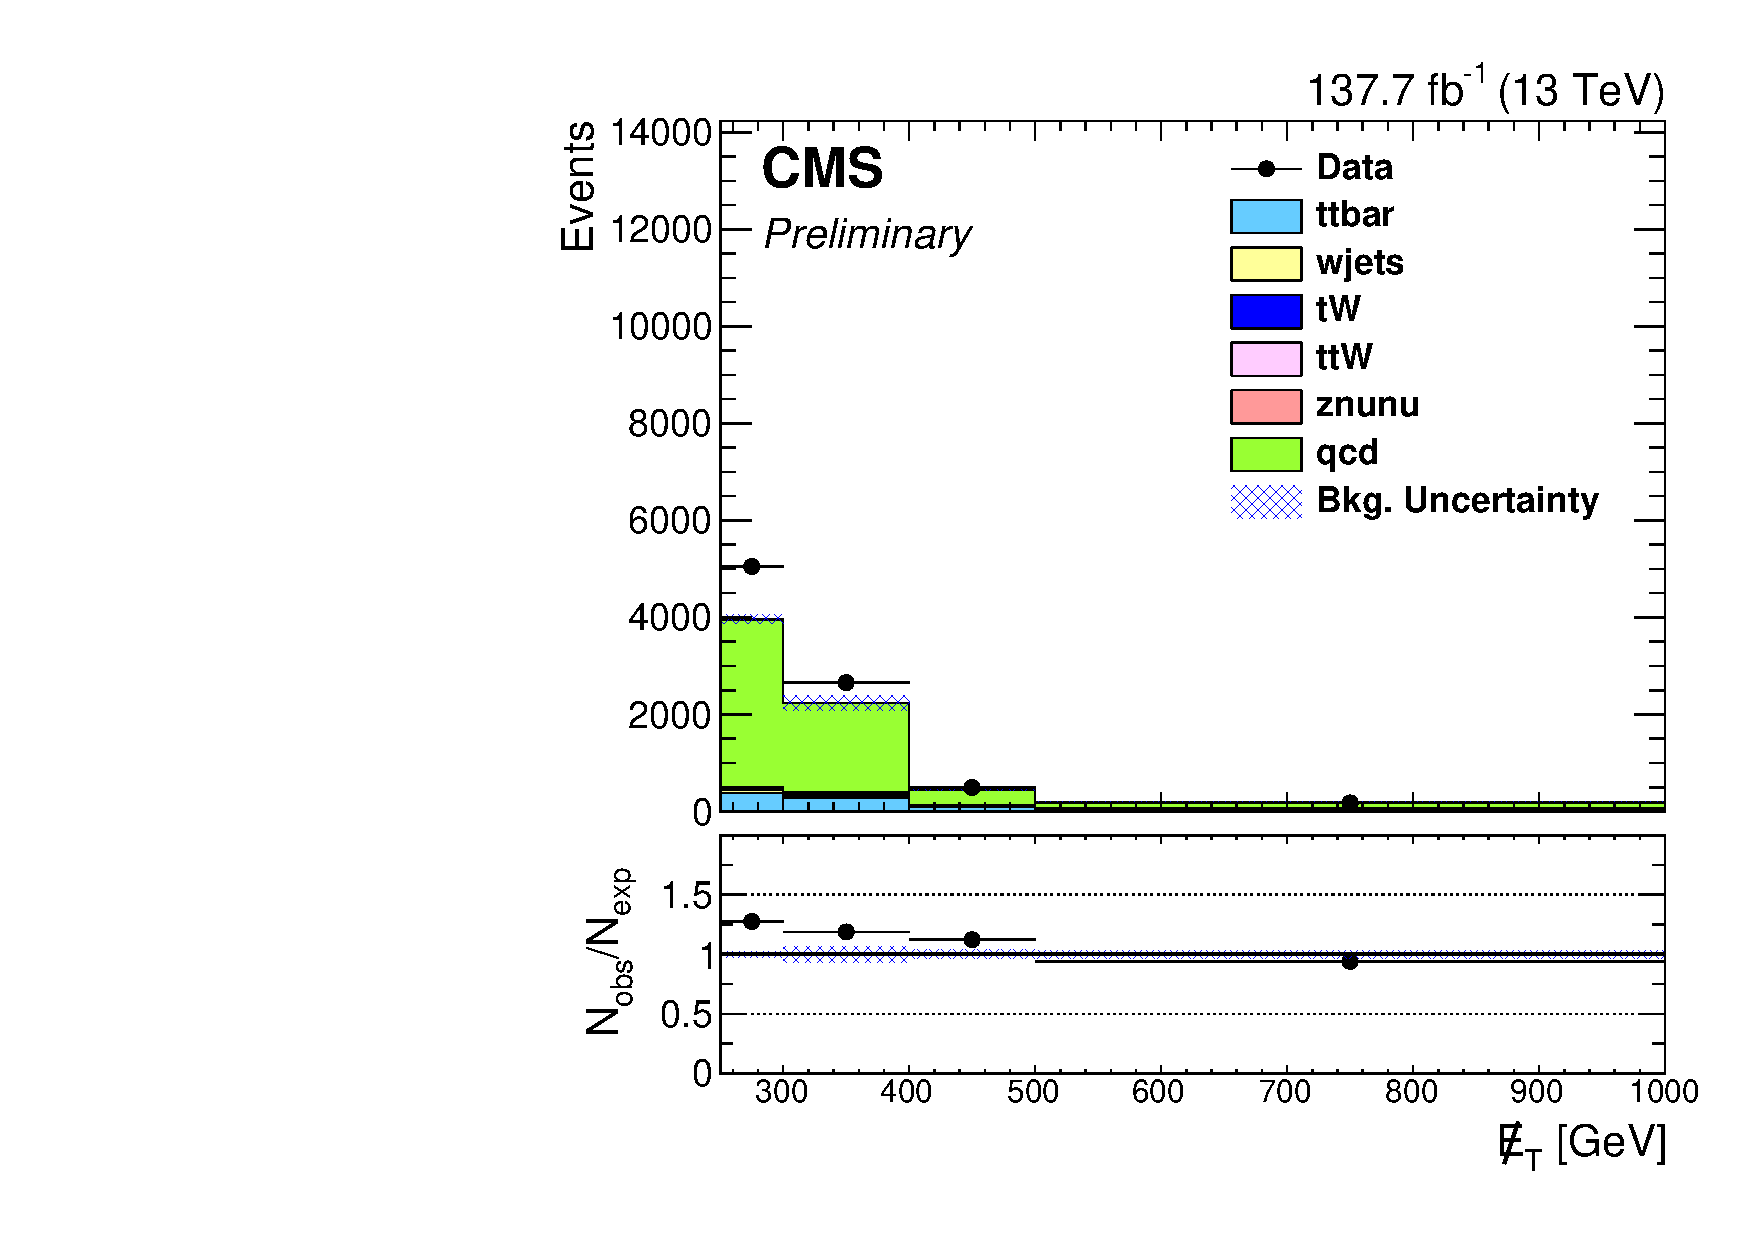
\includegraphics[width=0.32\textwidth]{../Research/SUSY/2019/LLB/lepcr_allEras/MET_pt_DataMC_hm_nb1_lowmtb_nj7_nrtgeq1__.pdf}
  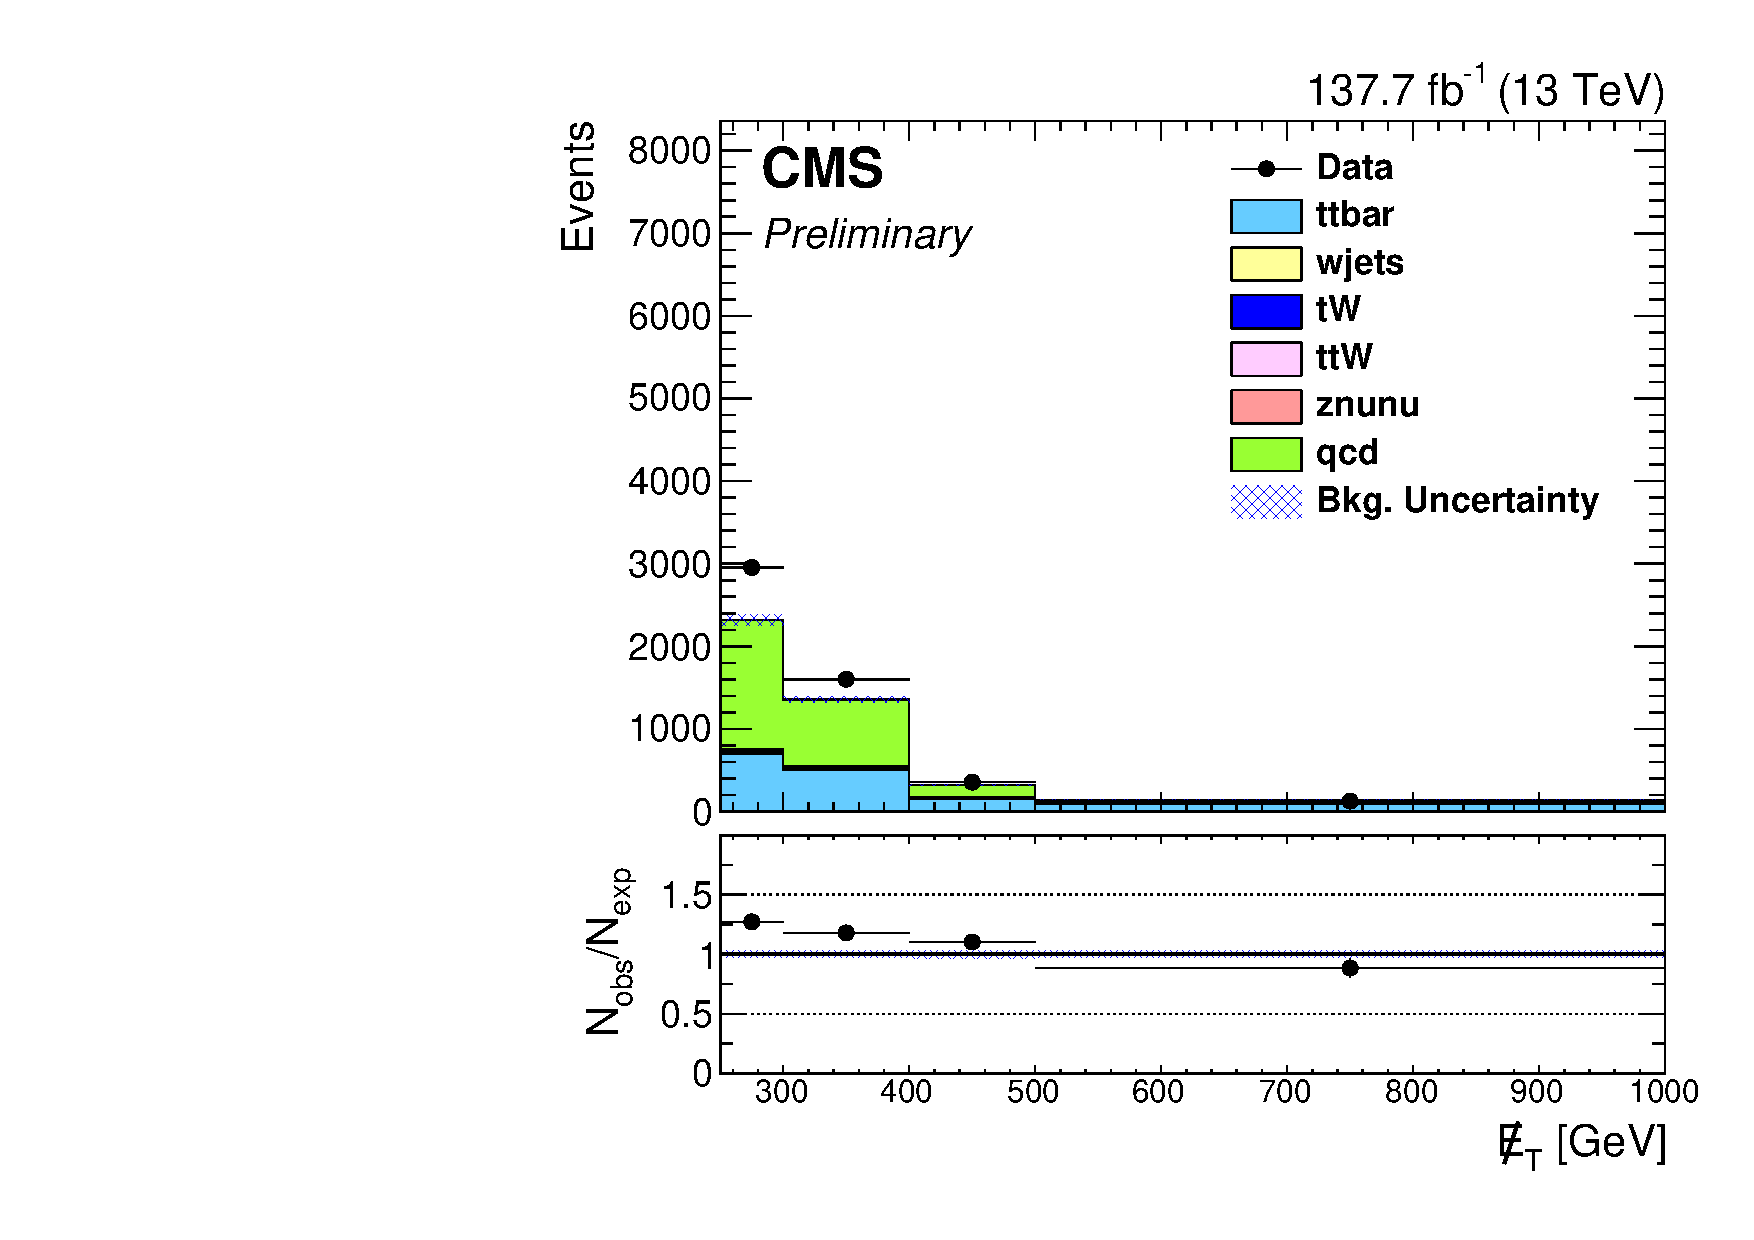
\includegraphics[width=0.32\textwidth]{../Research/SUSY/2019/LLB/lepcr_allEras/MET_pt_DataMC_hm_nb2_lowmtb_nj7_nrtgeq1__.pdf} \\
  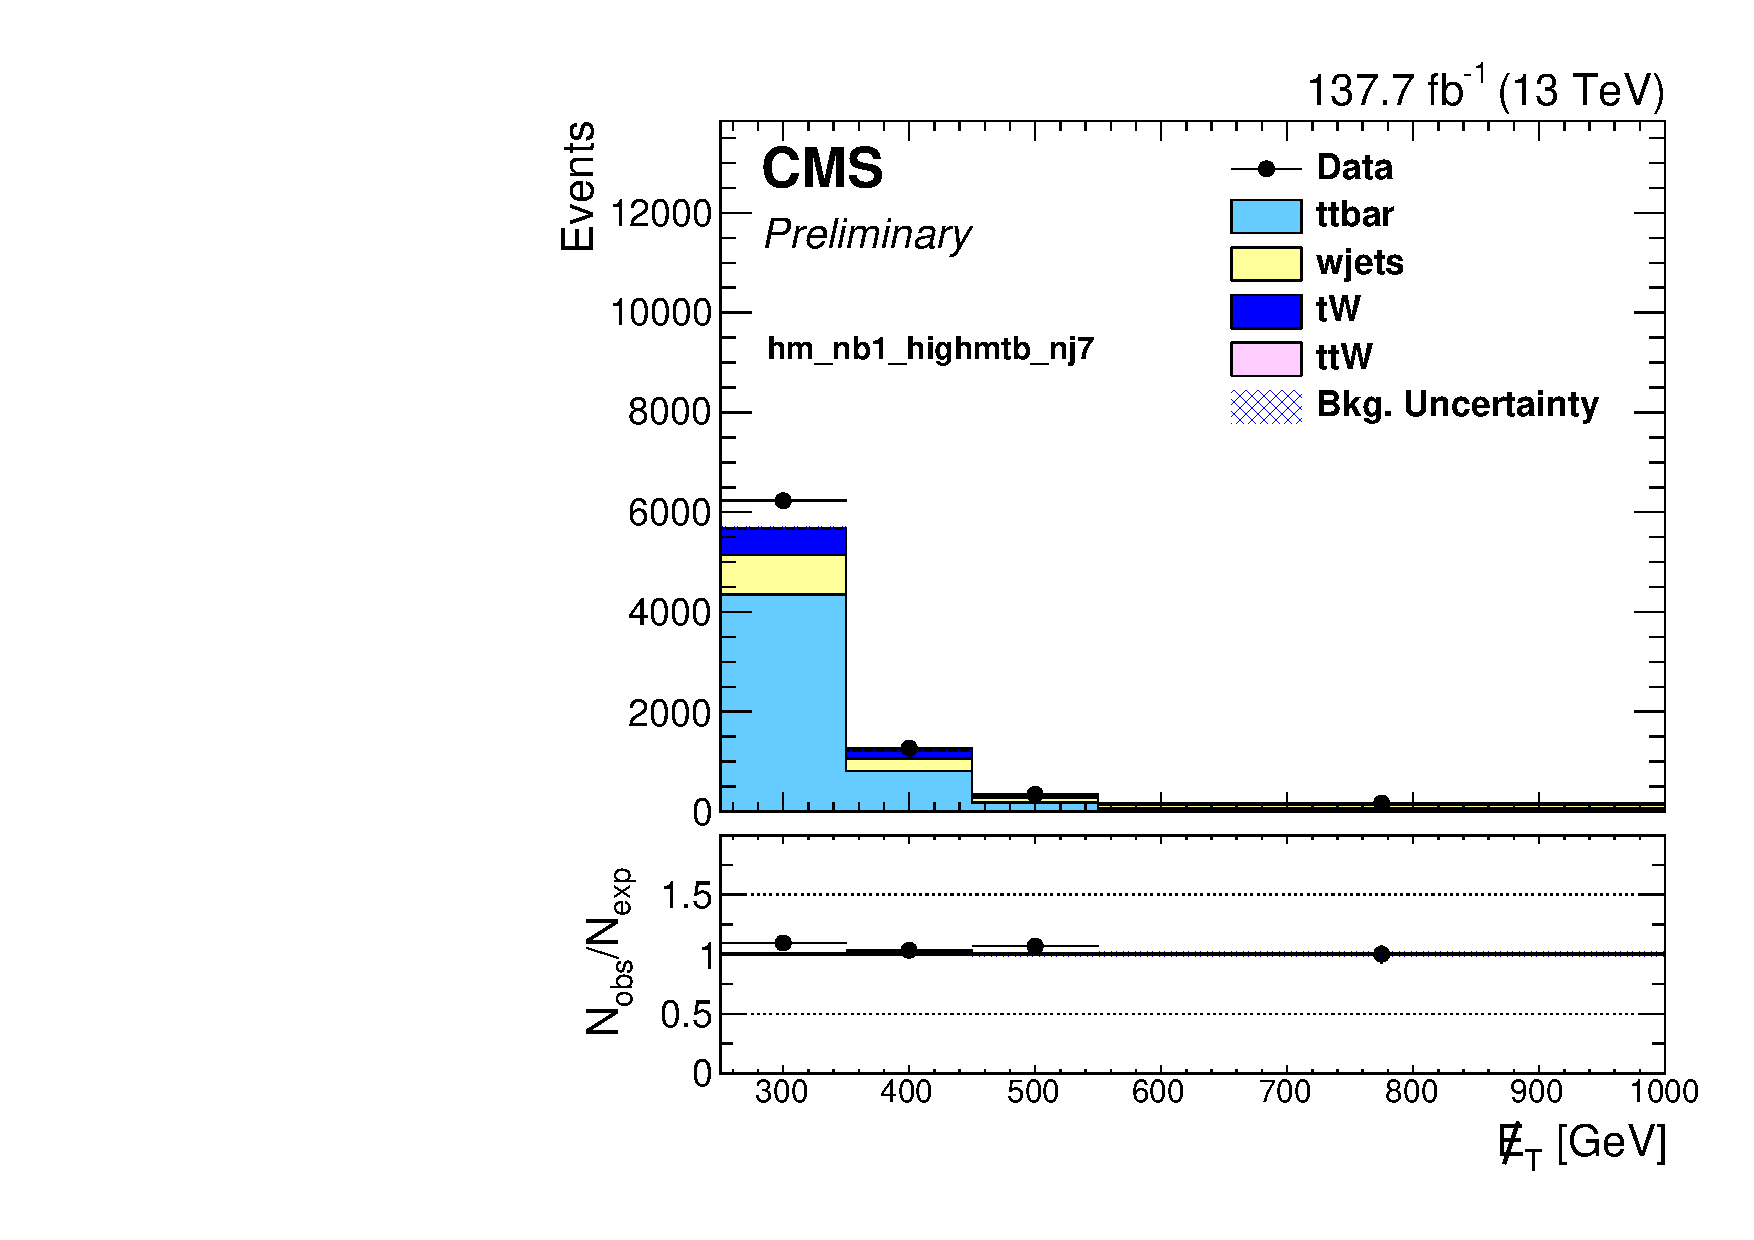
\includegraphics[width=0.32\textwidth]{../Research/SUSY/2019/LLB/lepcr_allEras/MET_pt_DataMC_hm_nb1_highmtb_nj7_nt0_nrt0_nw0__.pdf}
  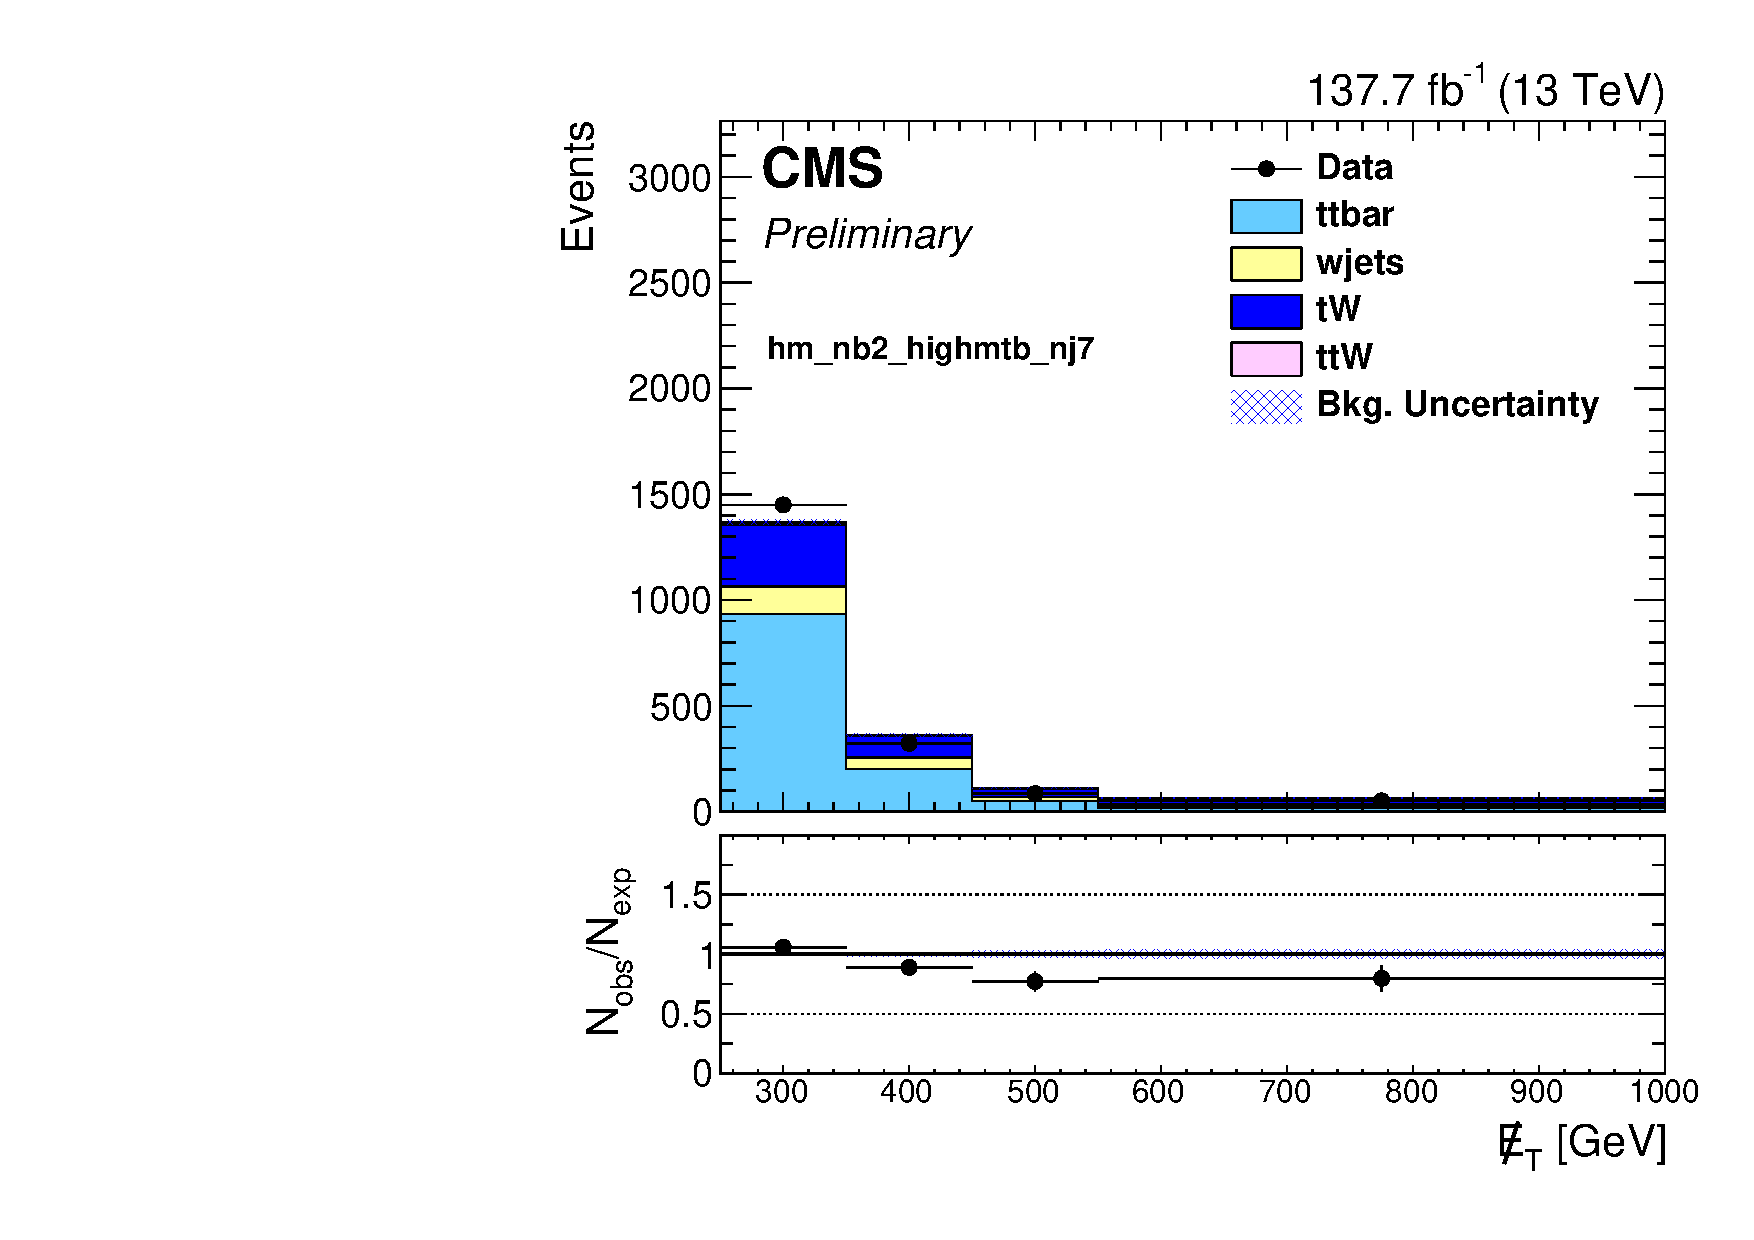
\includegraphics[width=0.32\textwidth]{../Research/SUSY/2019/LLB/lepcr_allEras/MET_pt_DataMC_hm_nb2_highmtb_nj7_nt0_nrt0_nw0__.pdf} \\
	\end{center}
	\caption{Comparison of the \met~distribution in the single-lepton sample after applying the high \dm~baseline selection in the $\mtb<175~\GeV$ and $\nt=0, \nrt=0,$ and $\nw=0$ region. Data and simulation are represented by the black points and stacked histograms, respectively. The error bars on the ratio of observed data to simulation correspond to the data statistical uncertainty and the shaded blue band represents the statistical uncertainty on the simulation. These regions are included with the search regions in the simultaneous fit for the signal extraction in order to estimate the LL contribution.
	 %               The plots in the top row are for events with $\mtb<175$~\GeV, with $5\leq\nj<7$ on the left and $\nj\geq7$ on the right. 
	 %               The plots in the middle row are for events with $\mtb>175$~\GeV and $\nt=0, \nw=0$, with $5\leq\nj<7$ on the left and $\nj\geq7$ on the right. 
	 %               The plot in the bottom row is for events with $\mtb>175$~\GeV and $\nj\geq5$, with $\nt=0, \nw\geq1$ on the left, $\nt\geq1, \nw=0$ on the middle, and $\nt\geq1$, and $\nw\geq1$ on the right.
	 }
	\label{fig:llb-1lcr-datavsmc-hm-nt0-nrt0-nw0}
\end{figure}

\begin{figure}[!htb]
	\begin{center}
  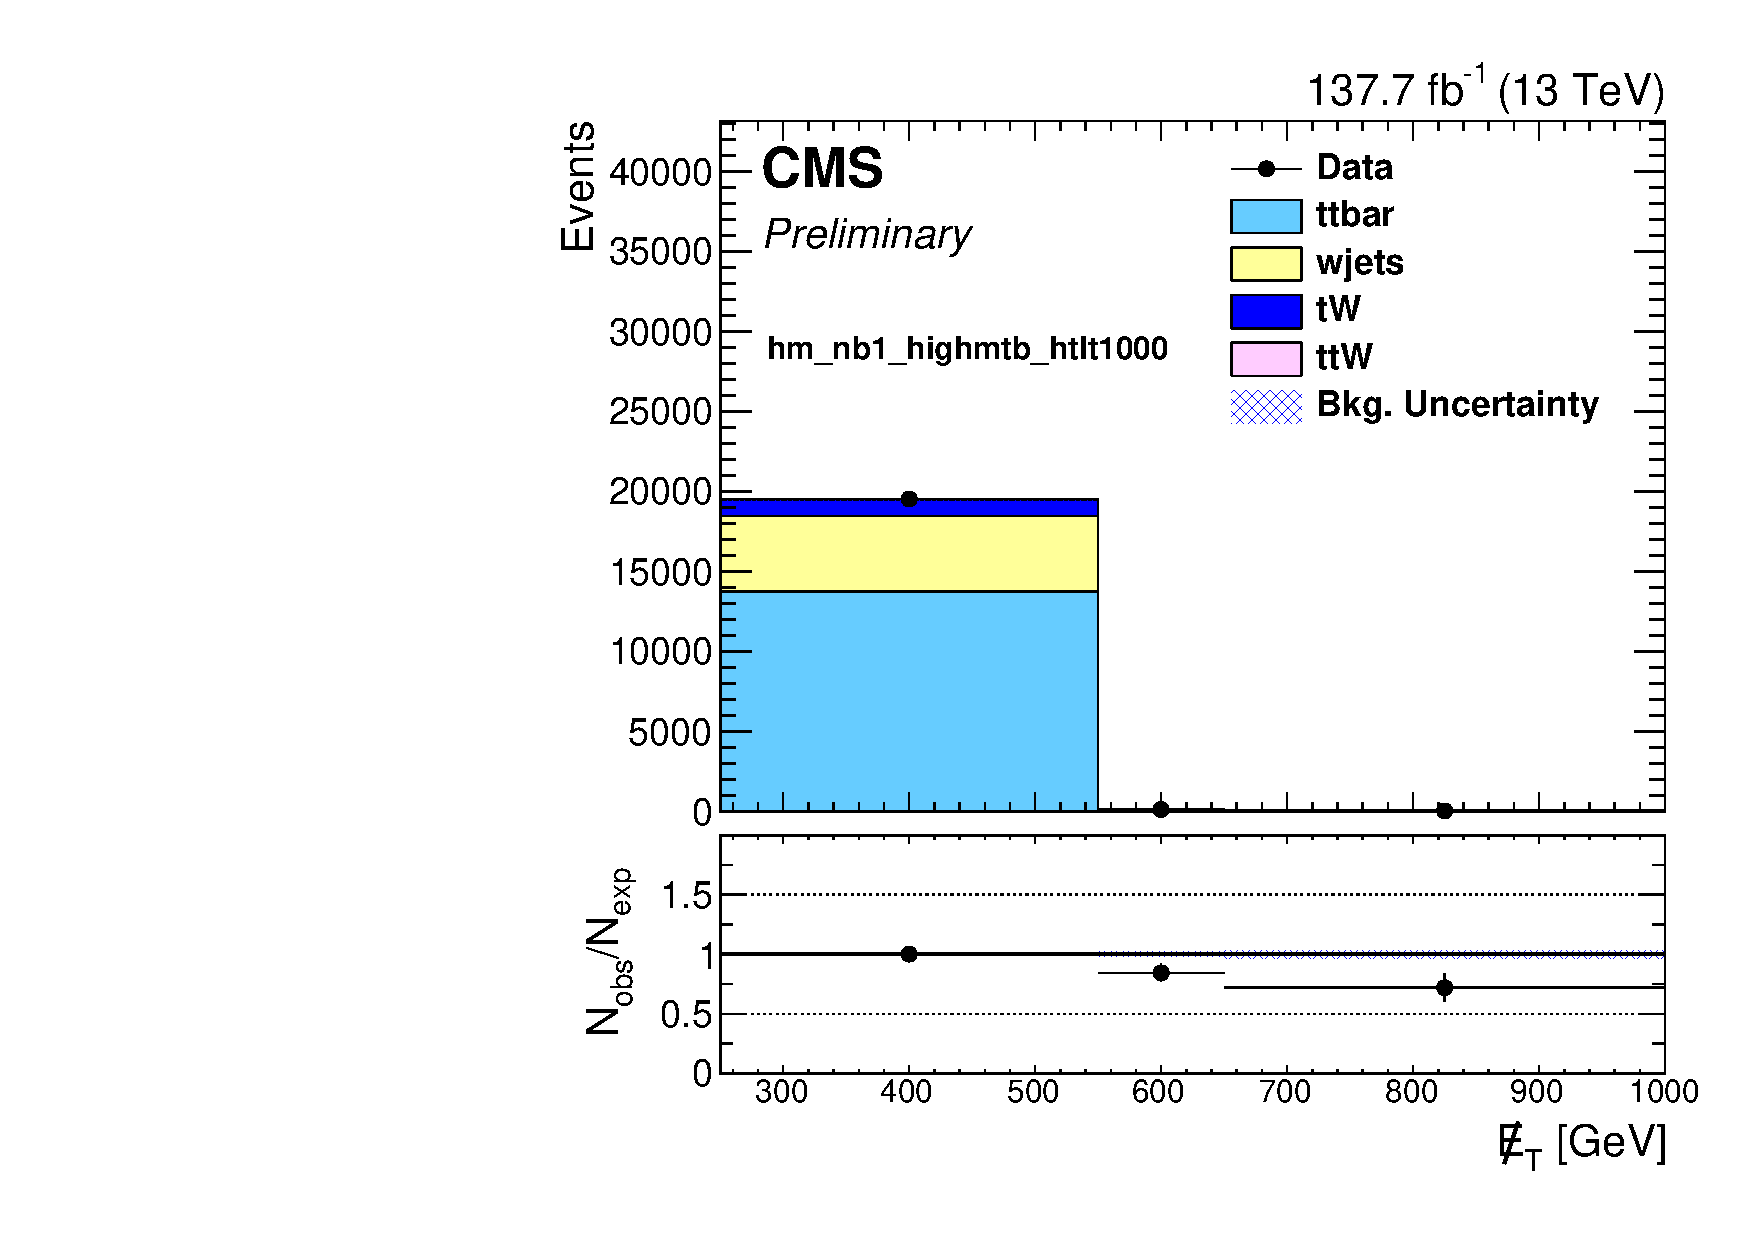
\includegraphics[width=0.32\textwidth]{../Research/SUSY/2019/LLB/lepcr_allEras/MET_pt_DataMC_hm_nb1_highmtb_ntgeq1_nrt0_nw0_htlt1000__.pdf}
  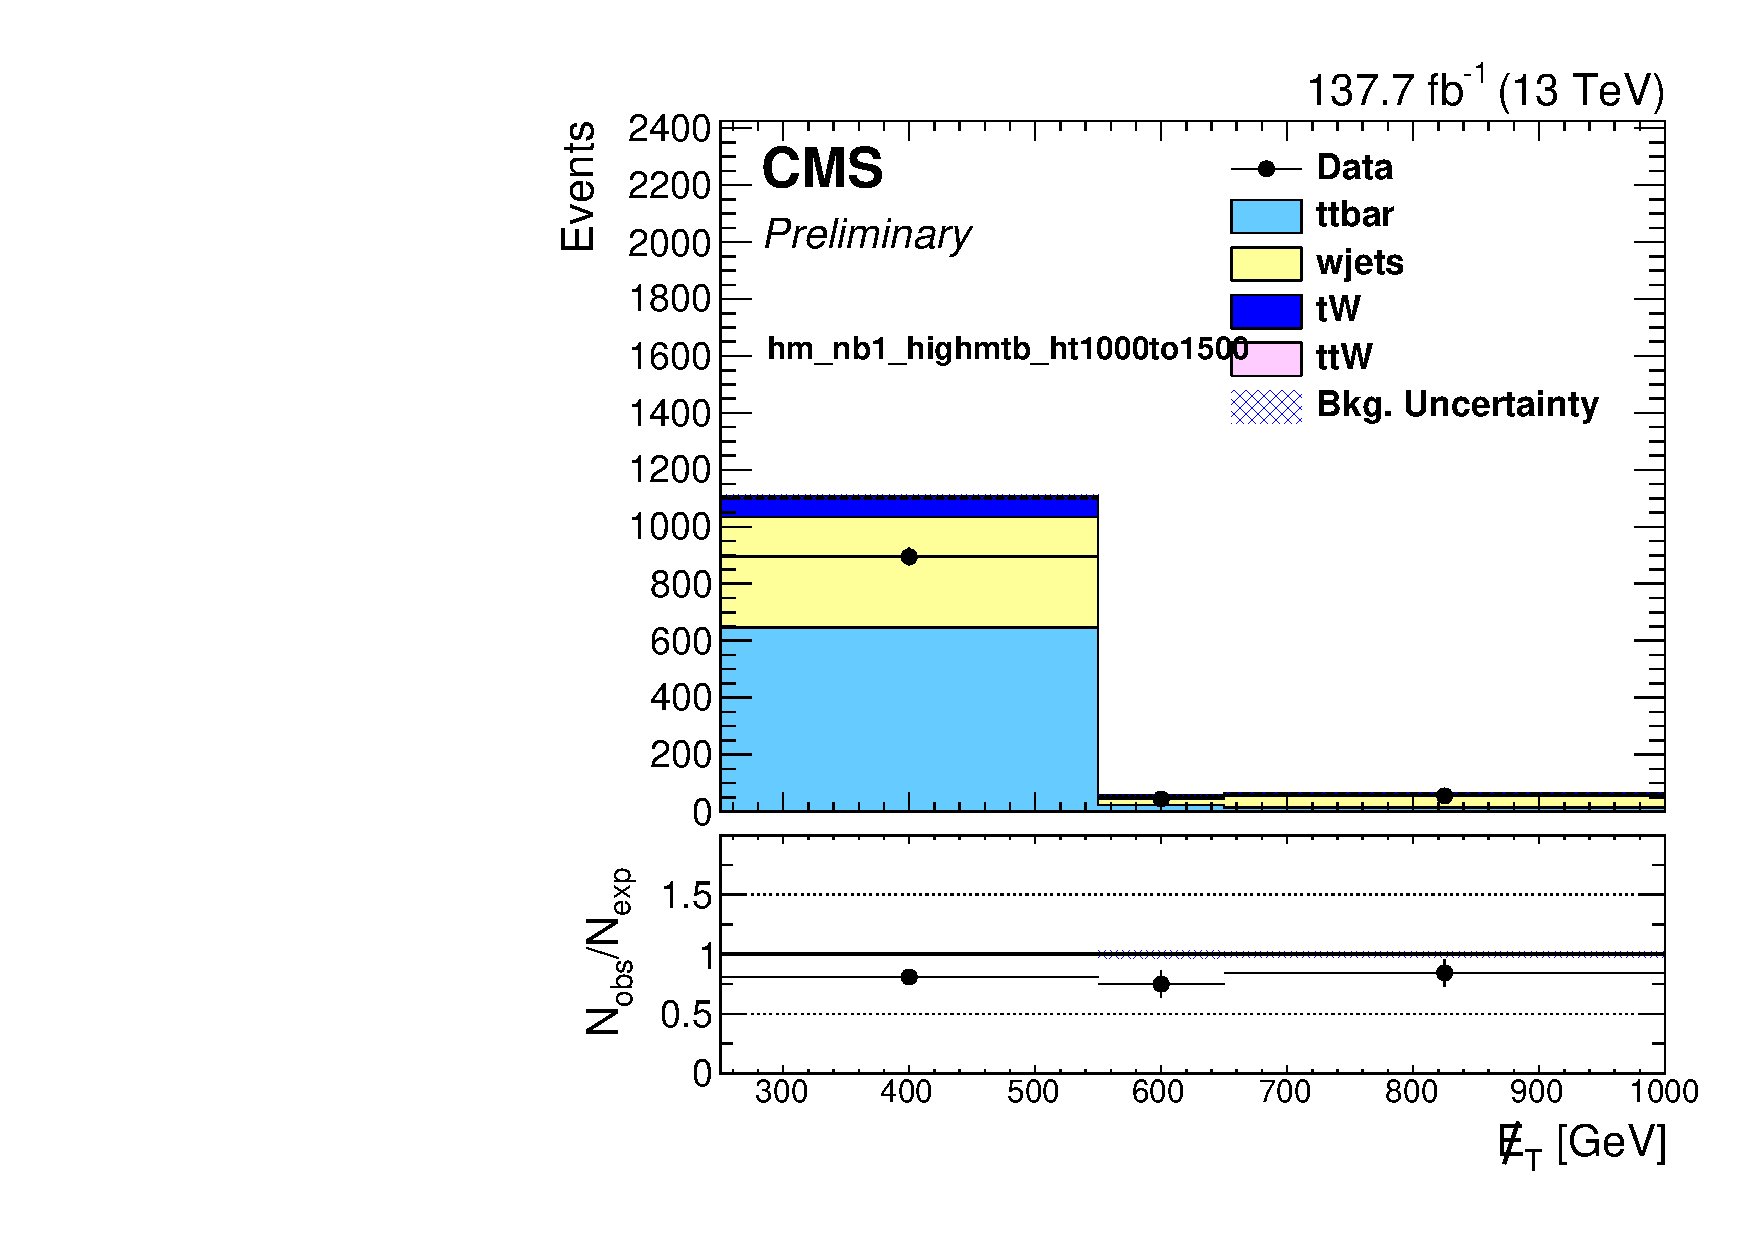
\includegraphics[width=0.32\textwidth]{../Research/SUSY/2019/LLB/lepcr_allEras/MET_pt_DataMC_hm_nb1_highmtb_ntgeq1_nrt0_nw0_ht1000to1500__.pdf}
  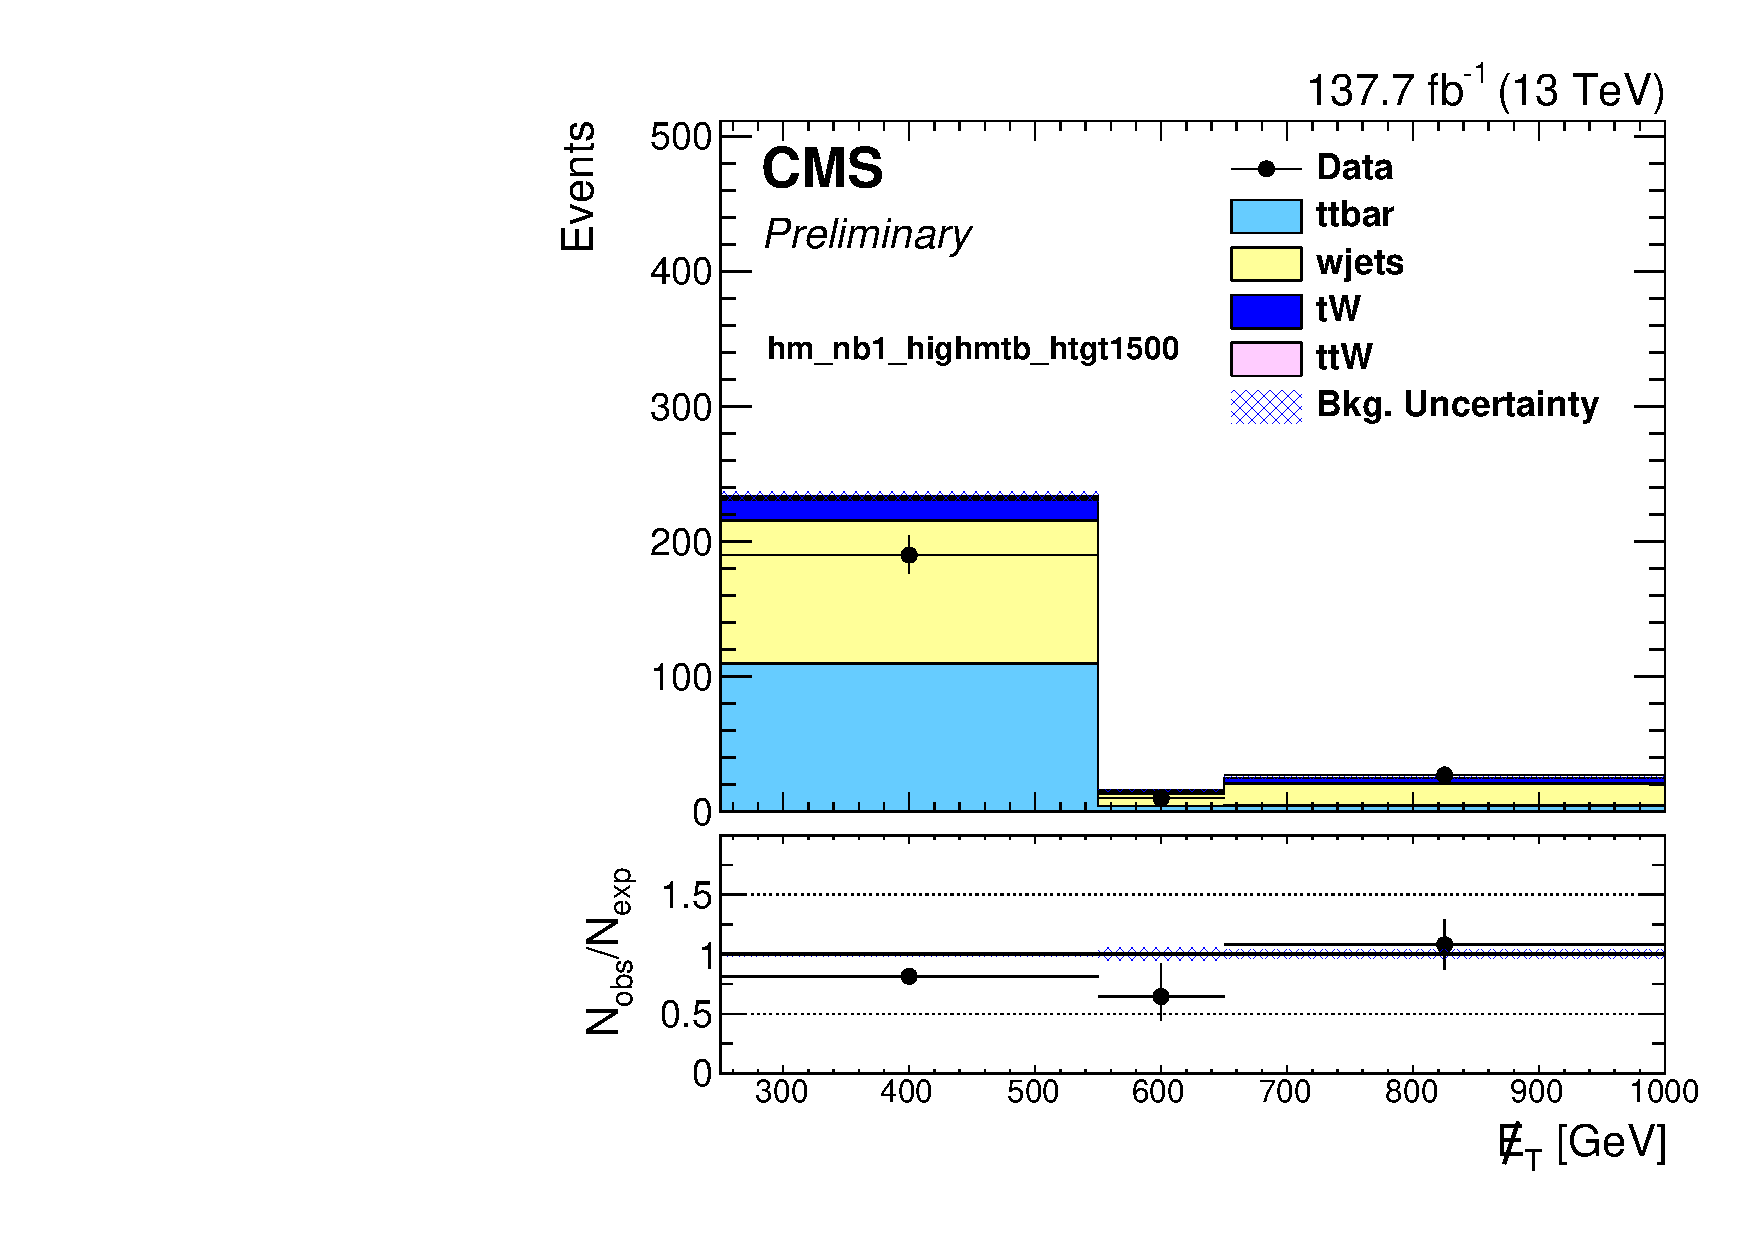
\includegraphics[width=0.32\textwidth]{../Research/SUSY/2019/LLB/lepcr_allEras/MET_pt_DataMC_hm_nb1_highmtb_ntgeq1_nrt0_nw0_htgt1500__.pdf} \\
  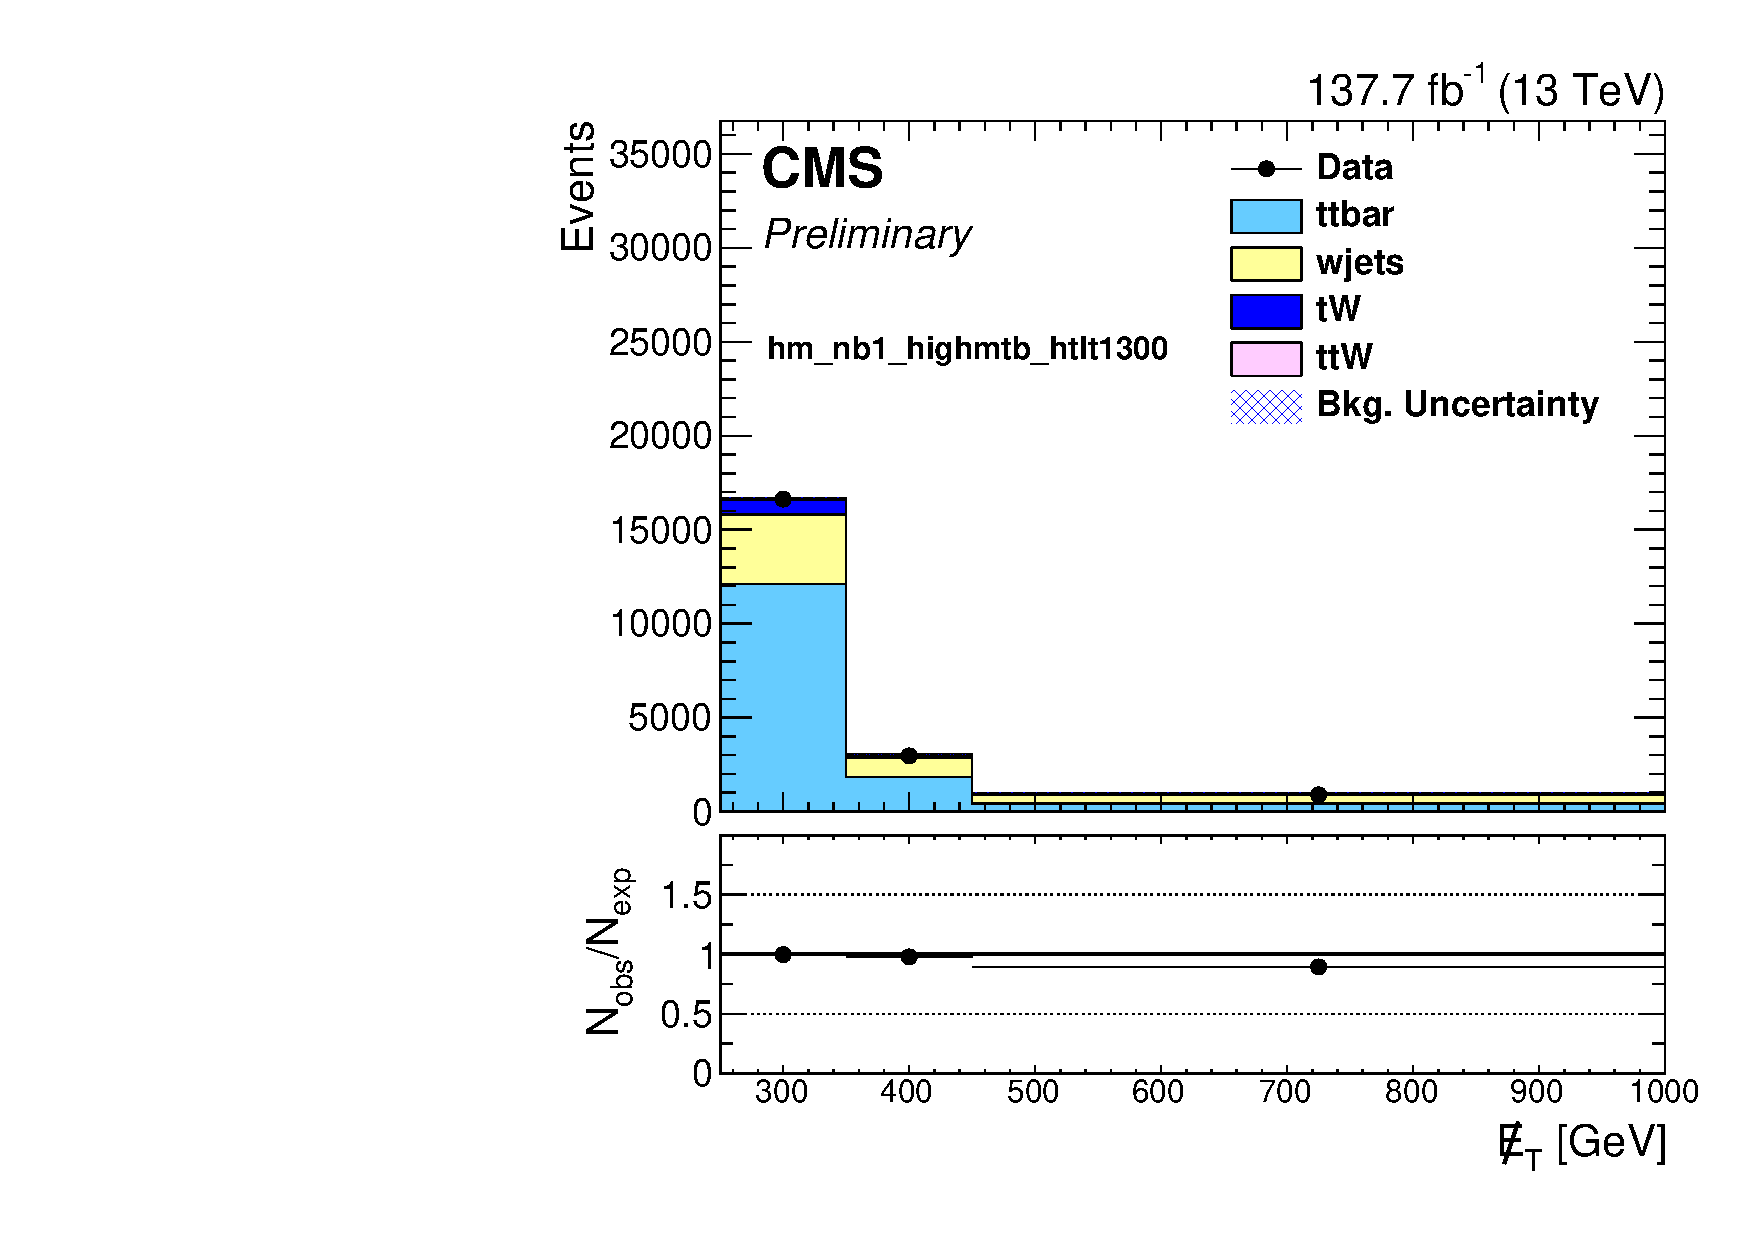
\includegraphics[width=0.32\textwidth]{../Research/SUSY/2019/LLB/lepcr_allEras/MET_pt_DataMC_hm_nb1_highmtb_nt0_nrt0_nwgeq1_htlt1300__.pdf} 
  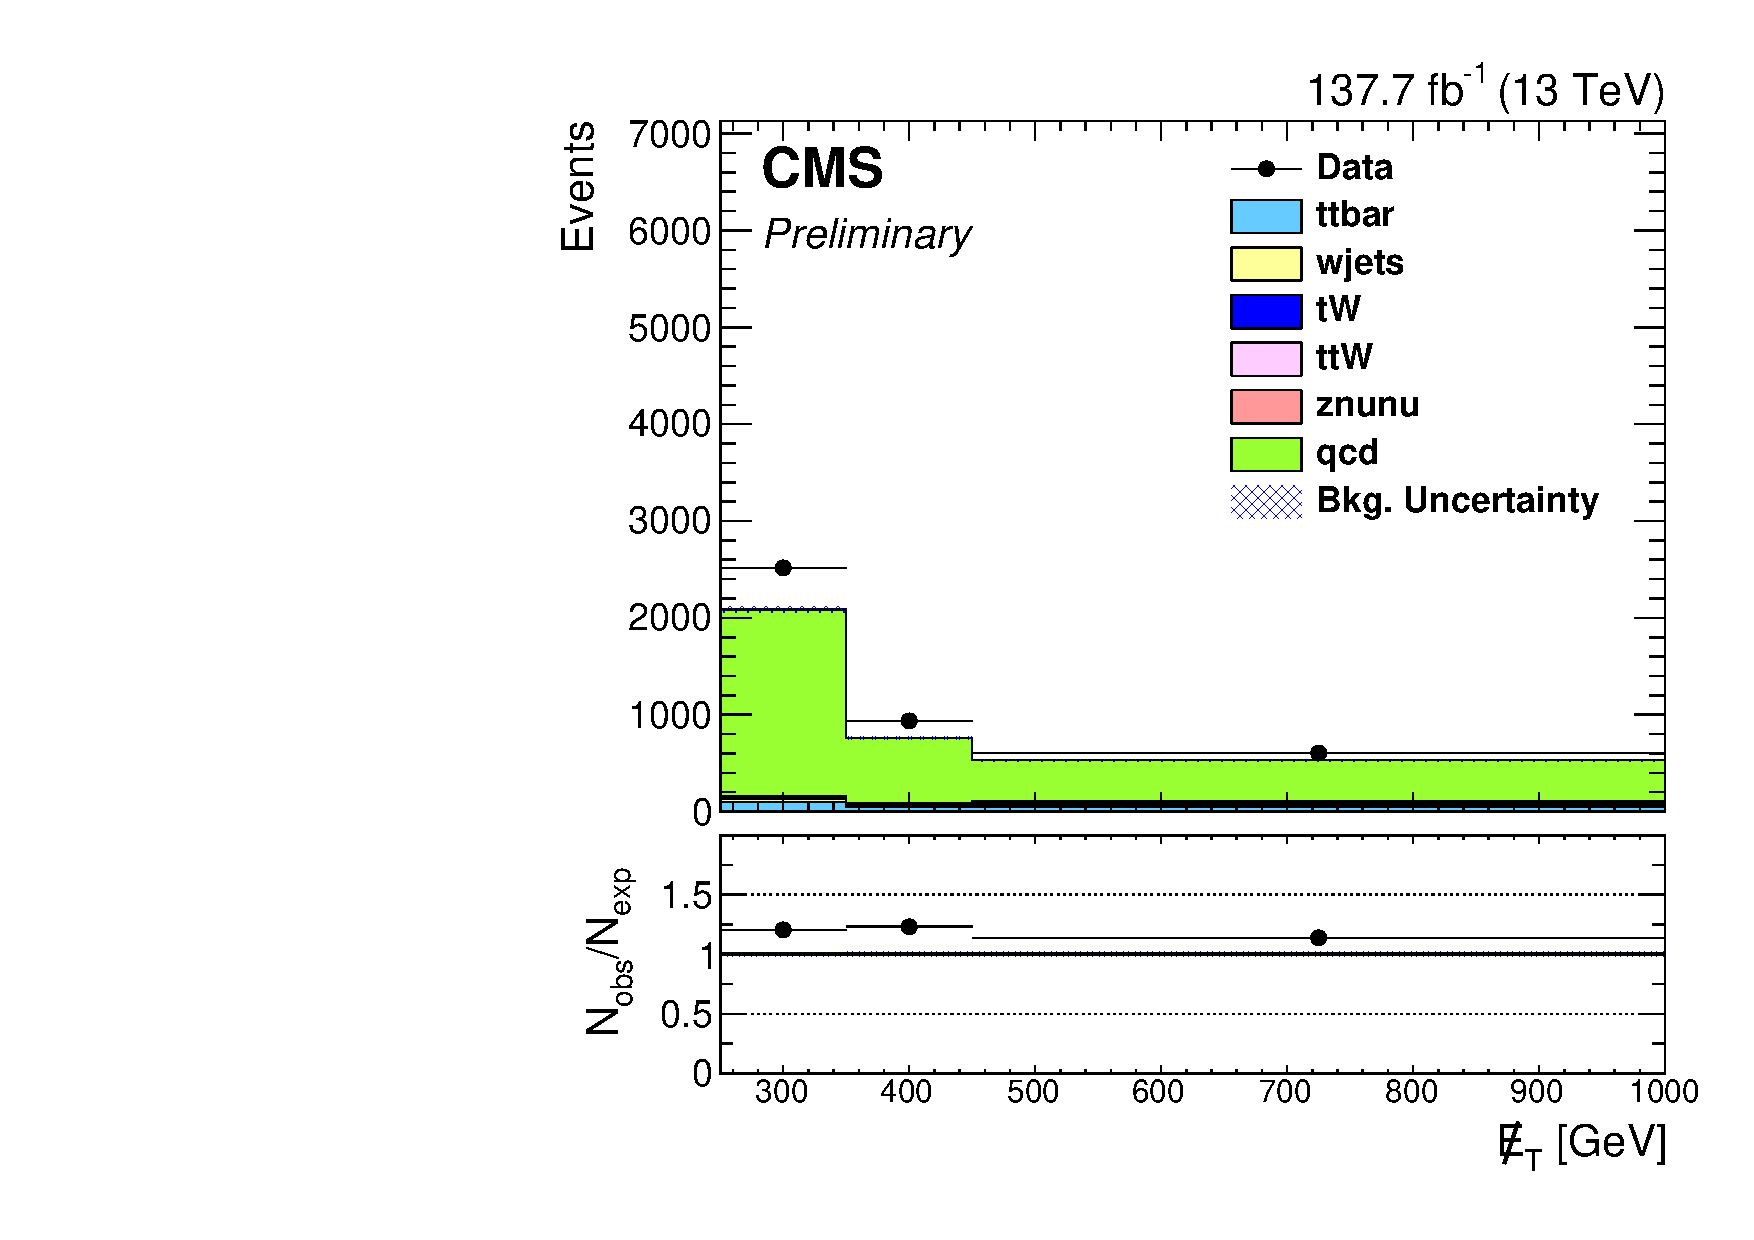
\includegraphics[width=0.32\textwidth]{../Research/SUSY/2019/LLB/lepcr_allEras/MET_pt_DataMC_hm_nb1_highmtb_nt0_nrt0_nwgeq1_htgt1300__.pdf} \\
  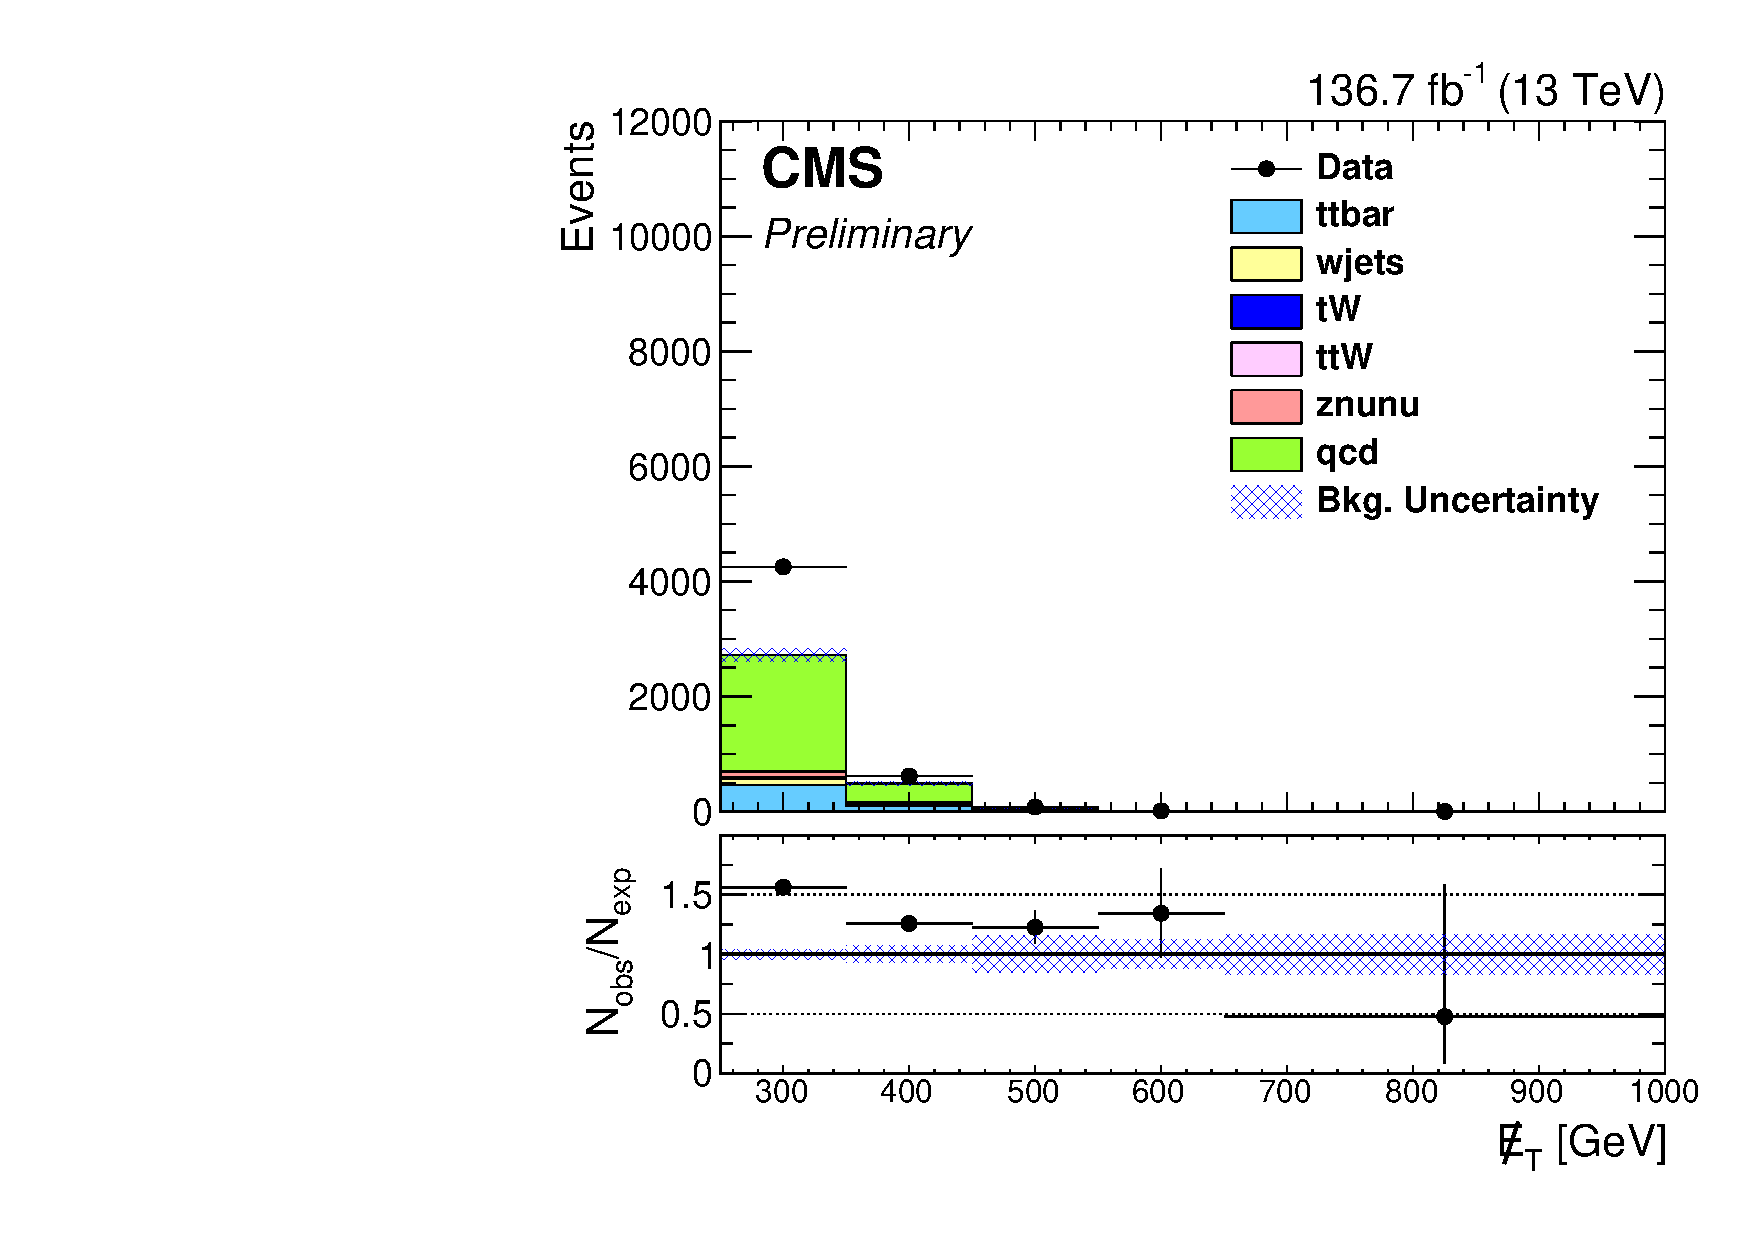
\includegraphics[width=0.32\textwidth]{../Research/SUSY/2019/LLB/lepcr_allEras/MET_pt_DataMC_hm_nb1_highmtb_nt0_nrtgeq1_nw0_htlt1000__.pdf} 
  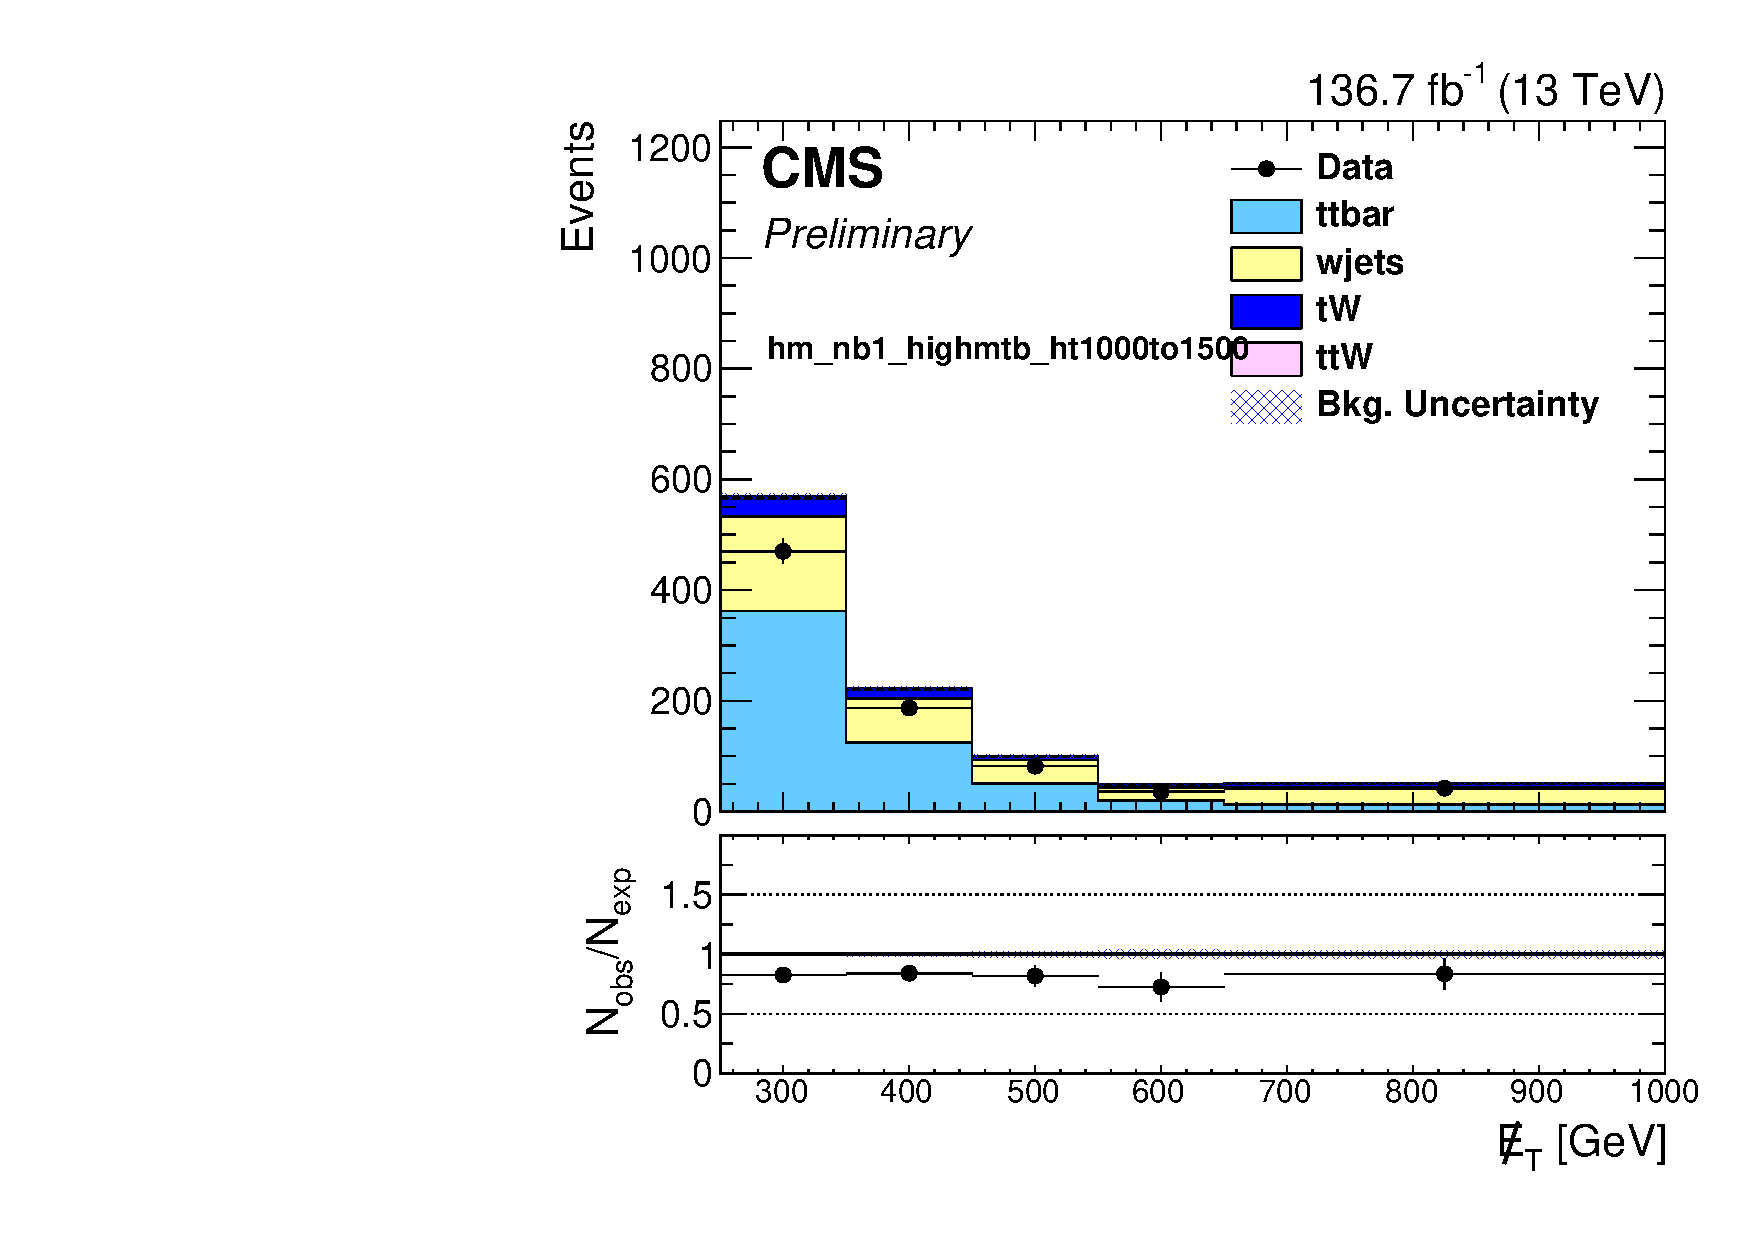
\includegraphics[width=0.32\textwidth]{../Research/SUSY/2019/LLB/lepcr_allEras/MET_pt_DataMC_hm_nb1_highmtb_nt0_nrtgeq1_nw0_ht1000to1500__.pdf} 
  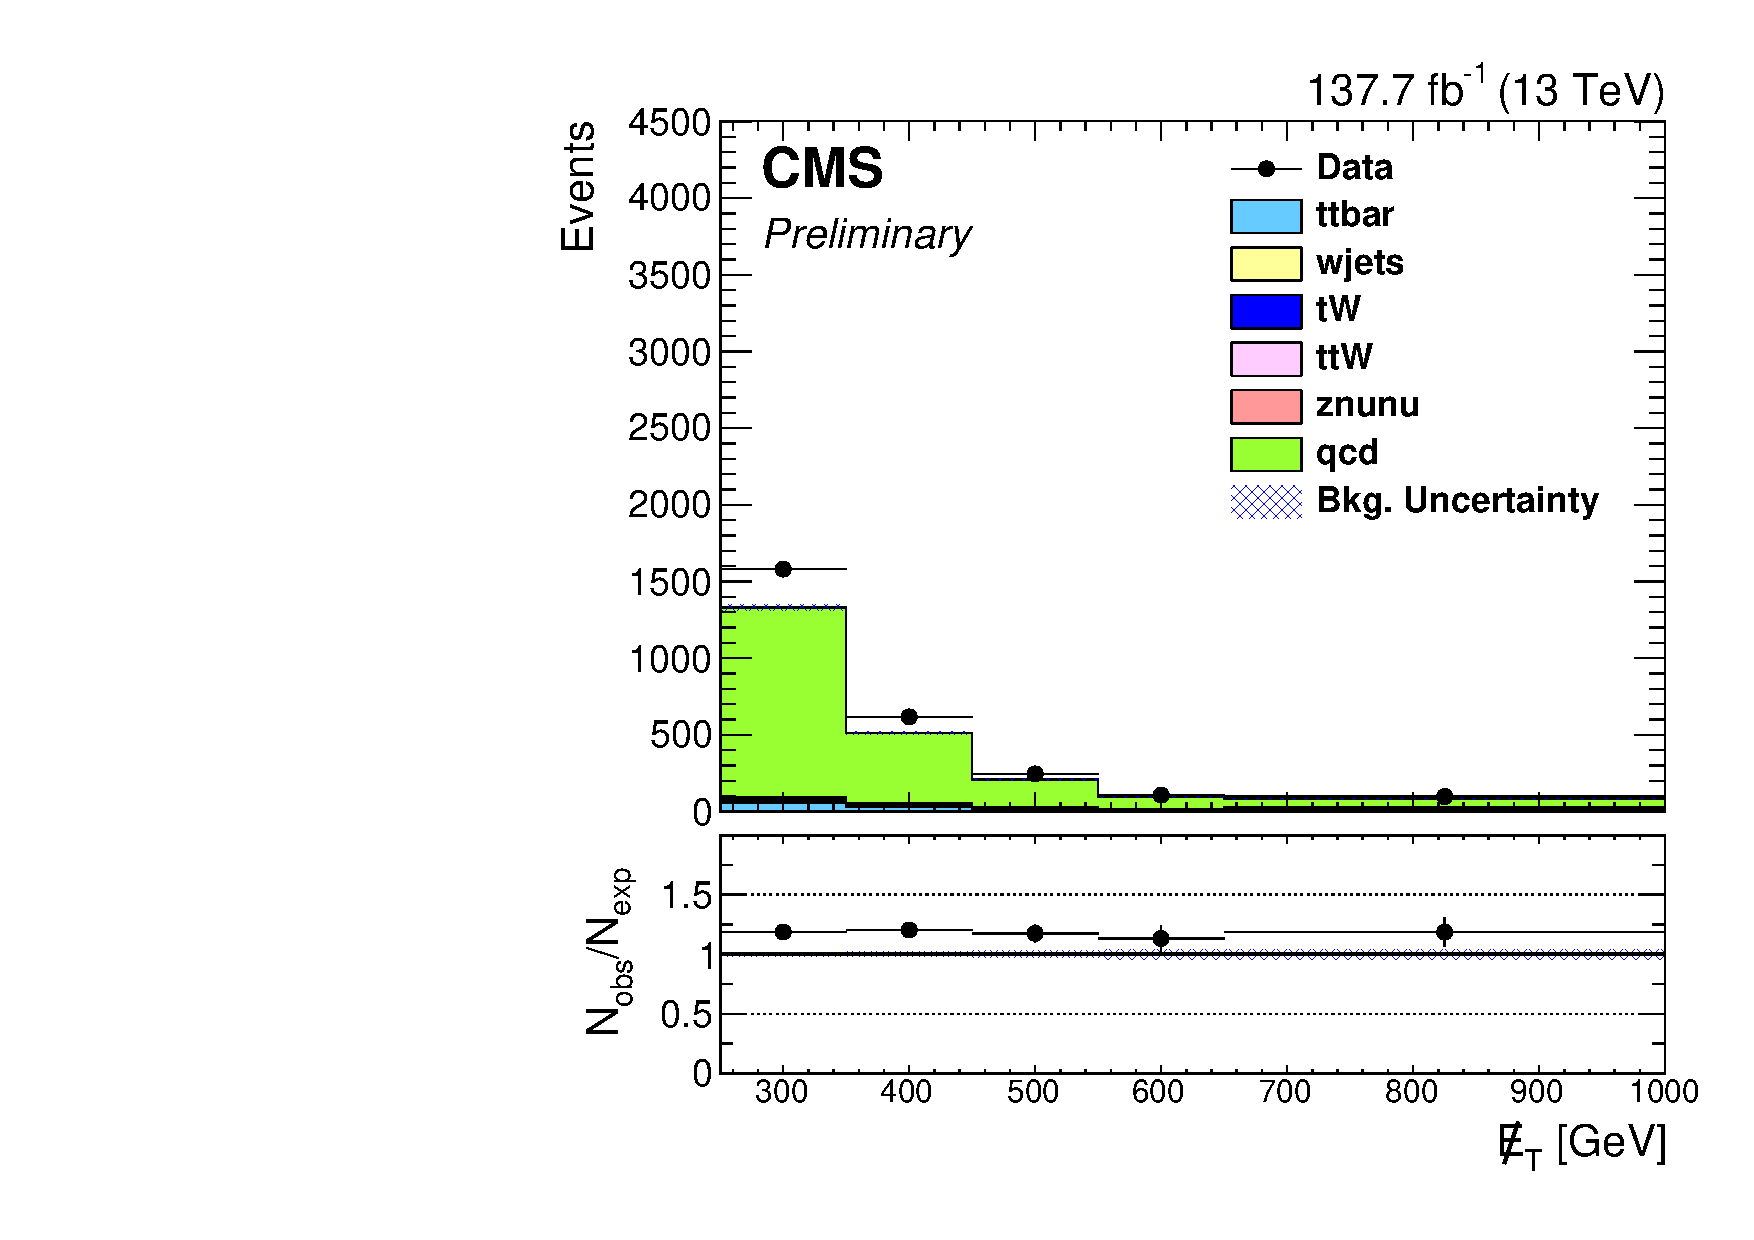
\includegraphics[width=0.32\textwidth]{../Research/SUSY/2019/LLB/lepcr_allEras/MET_pt_DataMC_hm_nb1_highmtb_nt0_nrtgeq1_nw0_htgt1500__.pdf} \\
  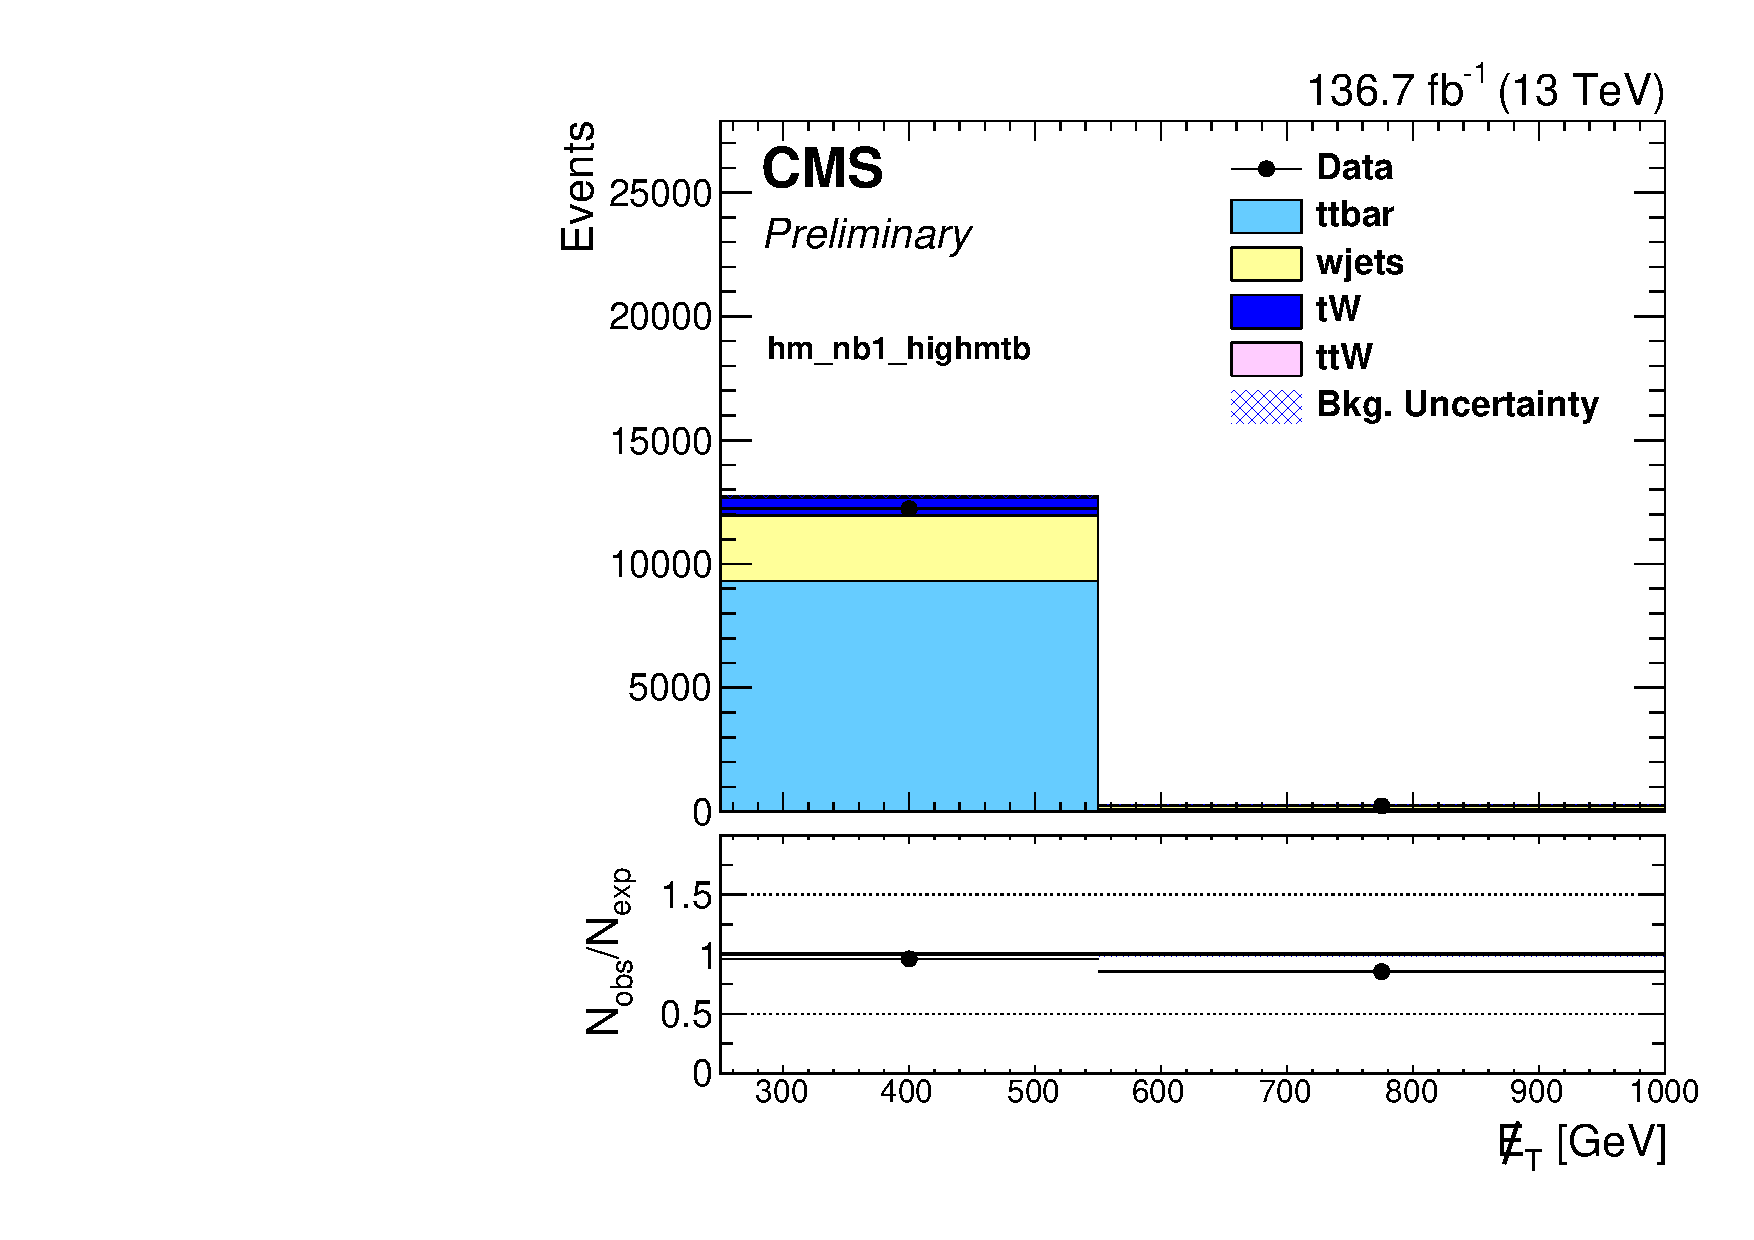
\includegraphics[width=0.32\textwidth]{../Research/SUSY/2019/LLB/lepcr_allEras/MET_pt_DataMC_hm_nb1_highmtb_ntgeq1_nrt0_nwgeq1__.pdf} 
  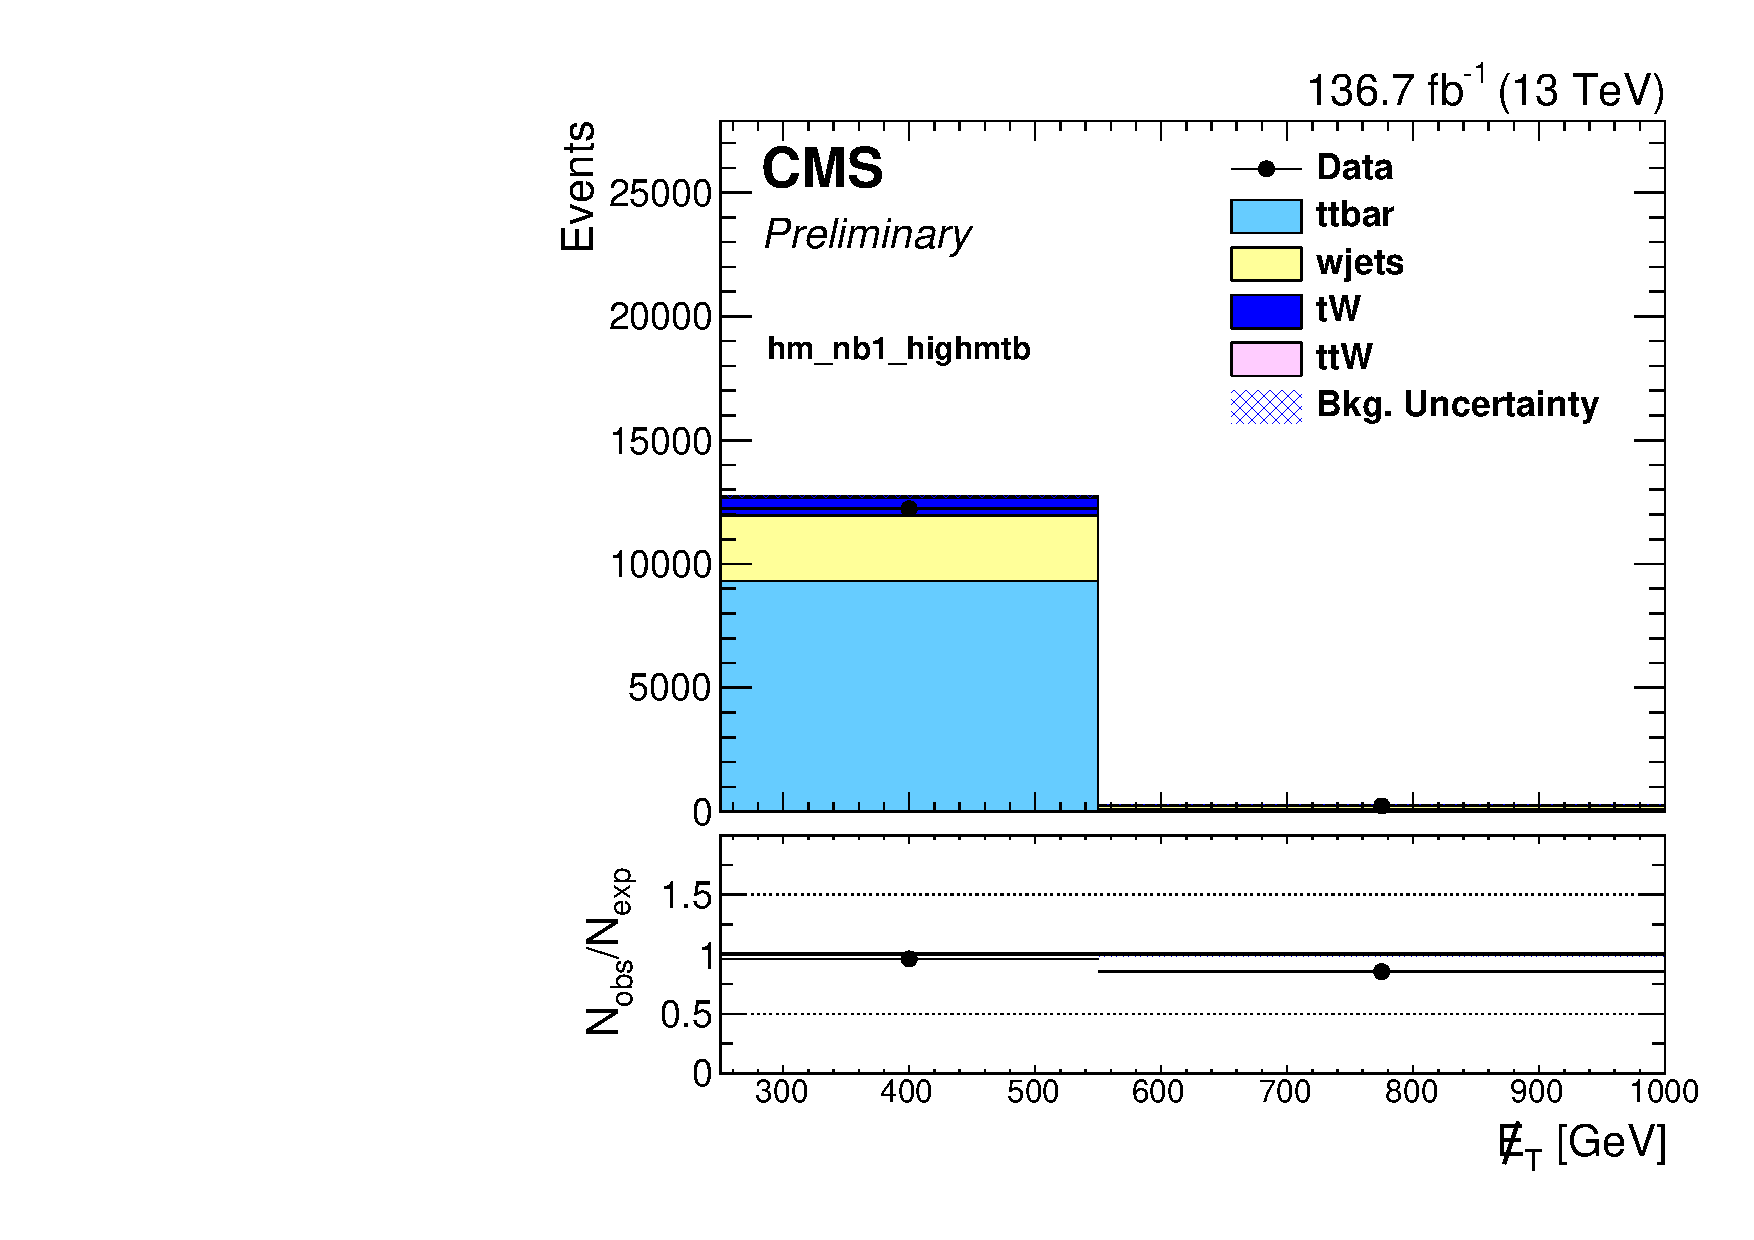
\includegraphics[width=0.32\textwidth]{../Research/SUSY/2019/LLB/lepcr_allEras/MET_pt_DataMC_hm_nb1_highmtb_ntgeq1_nrtgeq1_nw0__.pdf} 
  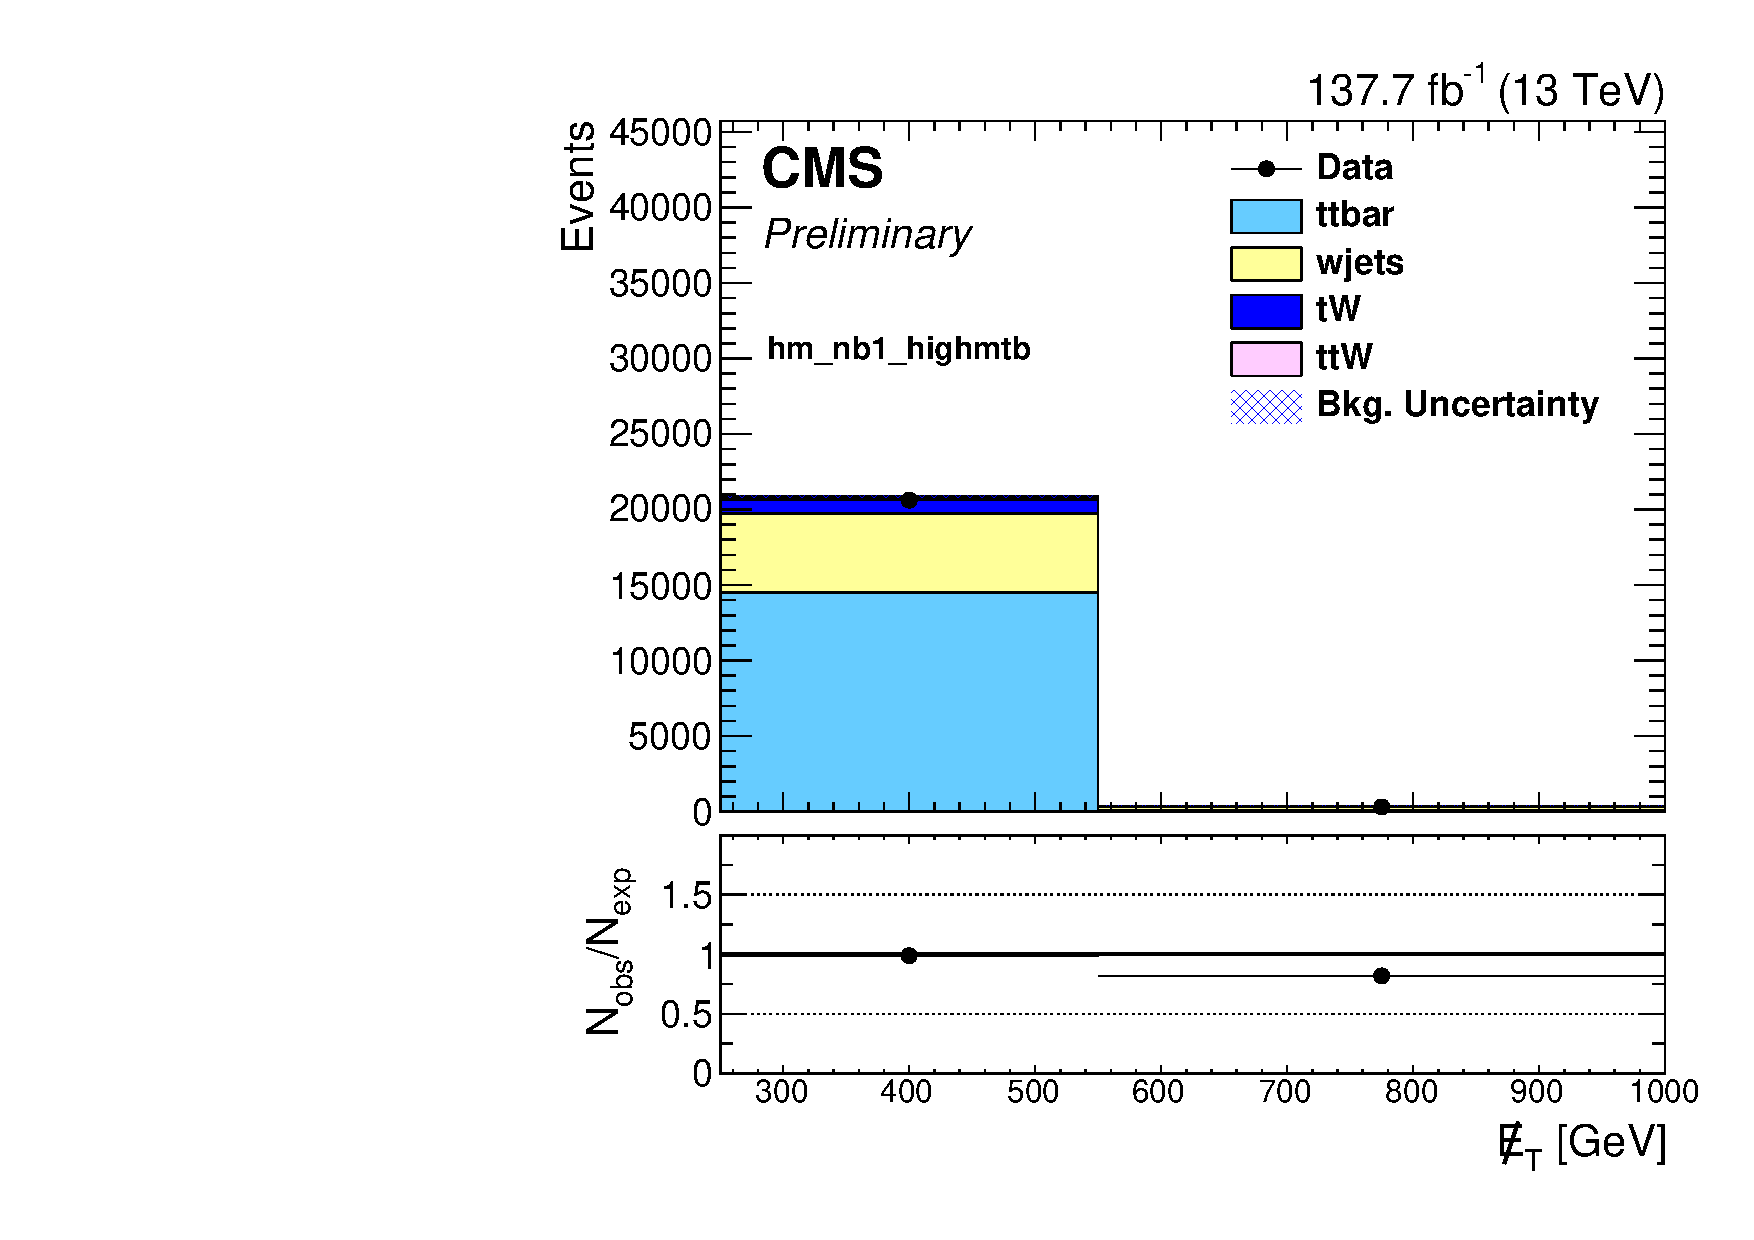
\includegraphics[width=0.32\textwidth]{../Research/SUSY/2019/LLB/lepcr_allEras/MET_pt_DataMC_hm_nb1_highmtb_nt0_nrtgeq1_nwgeq1__.pdf} \\
	\end{center}
	\caption{Comparison of the \met~distribution in the single-lepton sample after applying the high \dm~baseline selection in the $\nb=1$ region where there are $\geq1$ heavy object tags. Data and simulation are represented by the black points and stacked histograms, respectively. The error bars on the ratio of observed data to simulation correspo    nd to the data statistical uncertainty and the shaded blue band represents the statistical uncertainty on the simulation. These regions are included with the search regions in the simultaneous fit for the signal extraction in order to estimate the LL contribution.
	 %               The plots in the top row are for events with $\mtb<175$~\GeV, with $5\leq\nj<7$ on the left and $\nj\geq7$ on the right. 
	 %               The plots in the middle row are for events with $\mtb>175$~\GeV and $\nt=0, \nw=0$, with $5\leq\nj<7$ on the left and $\nj\geq7$ on the right. 
	 %               The plot in the bottom row is for events with $\mtb>175$~\GeV and $\nj\geq5$, with $\nt=0, \nw\geq1$ on the left, $\nt\geq1, \nw=0$ on the middle, and $\nt\geq1$, and $\nw\geq1$ on the right.
	 }
	\label{fig:llb-1lcr-datavsmc-hm-nb1}
\end{figure}

\begin{figure}[!htb]
	\begin{center}
  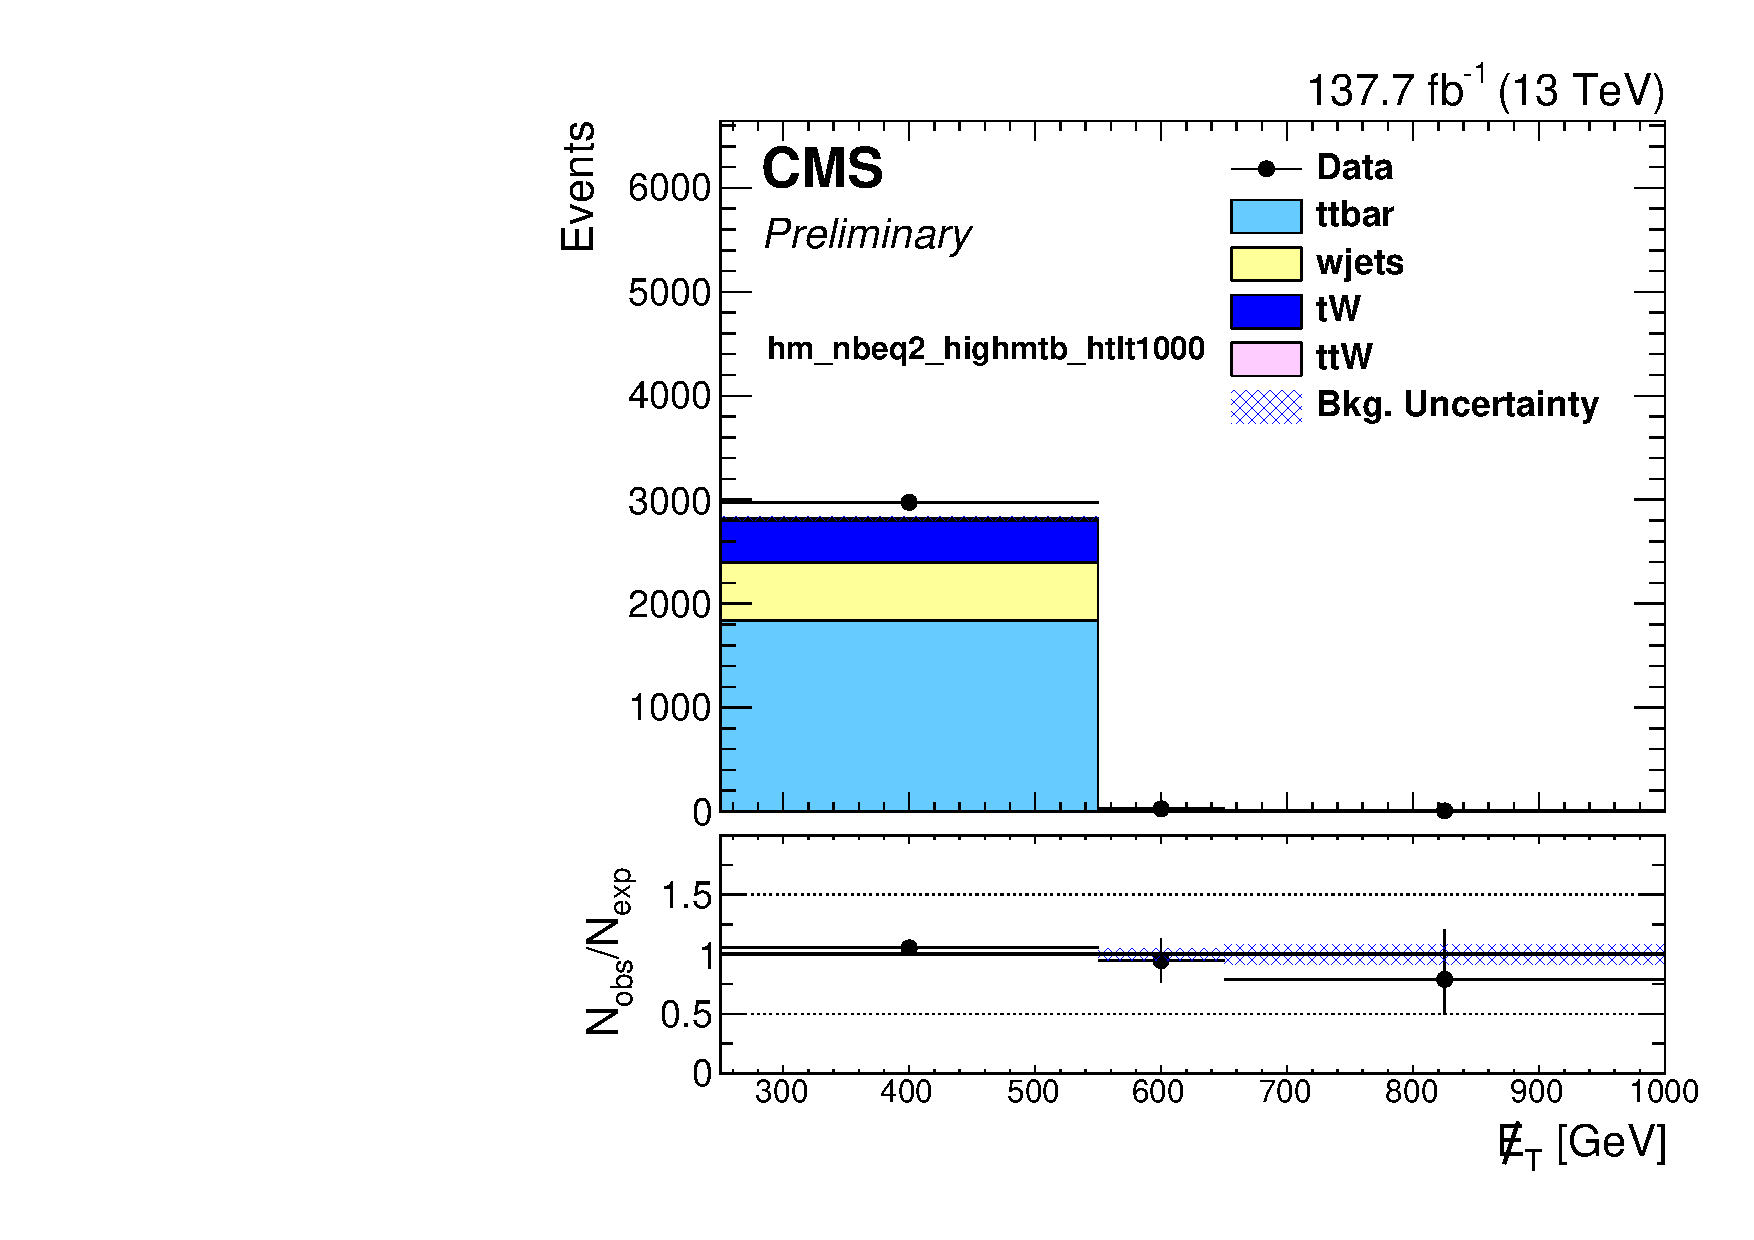
\includegraphics[width=0.32\textwidth]{../Research/SUSY/2019/LLB/lepcr_allEras/MET_pt_DataMC_hm_nbeq2_highmtb_nt1_nrt0_nw0_htlt1000__.pdf}
  \includegraphics[width=0.32\textwidth]{../Research/SUSY/2019/LLB/lepcr_allEras/MET_pt_DataMC_hm_nbeq2_highmtb_nt1_nrt0_nw0_ht1000to1500__.pdf}
  \includegraphics[width=0.32\textwidth]{../Research/SUSY/2019/LLB/lepcr_allEras/MET_pt_DataMC_hm_nbeq2_highmtb_nt1_nrt0_nw0_htgt1500__.pdf} \\
  \includegraphics[width=0.32\textwidth]{../Research/SUSY/2019/LLB/lepcr_allEras/MET_pt_DataMC_hm_nbeq2_highmtb_nt0_nrt0_nw1_htlt1300__.pdf} 
  \includegraphics[width=0.32\textwidth]{../Research/SUSY/2019/LLB/lepcr_allEras/MET_pt_DataMC_hm_nbeq2_highmtb_nt0_nrt0_nw1_htgt1300__.pdf} \\
  \includegraphics[width=0.32\textwidth]{../Research/SUSY/2019/LLB/lepcr_allEras/MET_pt_DataMC_hm_nbeq2_highmtb_nt0_nrt1_nw0_htlt1000__.pdf} 
  \includegraphics[width=0.32\textwidth]{../Research/SUSY/2019/LLB/lepcr_allEras/MET_pt_DataMC_hm_nbeq2_highmtb_nt0_nrt1_nw0_ht1000to1500__.pdf} 
  \includegraphics[width=0.32\textwidth]{../Research/SUSY/2019/LLB/lepcr_allEras/MET_pt_DataMC_hm_nbeq2_highmtb_nt0_nrt1_nw0_htgt1500__.pdf} \\
  \includegraphics[width=0.32\textwidth]{../Research/SUSY/2019/LLB/lepcr_allEras/MET_pt_DataMC_hm_nbeq2_highmtb_nt1_nrt0_nw1__.pdf} 
  \includegraphics[width=0.32\textwidth]{../Research/SUSY/2019/LLB/lepcr_allEras/MET_pt_DataMC_hm_nbeq2_highmtb_nt0_nrt1_nw1__.pdf} \\
	\end{center}
	\caption{Comparison of the \met~distribution in the single-lepton sample after applying the high \dm~baseline selection in the $\nb=2$ and $\nt=1, \nrt=1,$ or $\nw=1$ regions. Data and simulation are represented by the black points and stacked histograms, respectively. The error bars on the ratio of observed data to simulation correspo    nd to the data statistical uncertainty and the shaded blue band represents the statistical uncertainty on the simulation. These regions are included with the search regions in the simultaneous fit for the signal extraction in order to estimate the LL contribution.
	 %               The plots in the top row are for events with $\mtb<175$~\GeV, with $5\leq\nj<7$ on the left and $\nj\geq7$ on the right. 
	 %               The plots in the middle row are for events with $\mtb>175$~\GeV and $\nt=0, \nw=0$, with $5\leq\nj<7$ on the left and $\nj\geq7$ on the right. 
	 %               The plot in the bottom row is for events with $\mtb>175$~\GeV and $\nj\geq5$, with $\nt=0, \nw\geq1$ on the left, $\nt\geq1, \nw=0$ on the middle, and $\nt\geq1$, and $\nw\geq1$ on the right.
	 }
	\label{fig:llb-1lcr-datavsmc-hm-nb2-1}
\end{figure}

\begin{figure}[!htb]
	\begin{center}
  \includegraphics[width=0.32\textwidth]{../Research/SUSY/2019/LLB/lepcr_allEras/MET_pt_DataMC_hm_nbeq2_highmtb_nt1_nrt1_nw0_htlt1300__.pdf}
  \includegraphics[width=0.32\textwidth]{../Research/SUSY/2019/LLB/lepcr_allEras/MET_pt_DataMC_hm_nbeq2_highmtb_nt1_nrt1_nw0_htgt1300__.pdf} \\
  \includegraphics[width=0.32\textwidth]{../Research/SUSY/2019/LLB/lepcr_allEras/MET_pt_DataMC_hm_nbeq2_highmtb_nt2_nrt0_nw0_htlt1300__.pdf}
  \includegraphics[width=0.32\textwidth]{../Research/SUSY/2019/LLB/lepcr_allEras/MET_pt_DataMC_hm_nbeq2_highmtb_nt2_nrt0_nw0_htgt1300__.pdf} 
  \includegraphics[width=0.32\textwidth]{../Research/SUSY/2019/LLB/lepcr_allEras/MET_pt_DataMC_hm_nbeq2_highmtb_nt0_nrt0_nw2__.pdf} \\
  \includegraphics[width=0.32\textwidth]{../Research/SUSY/2019/LLB/lepcr_allEras/MET_pt_DataMC_hm_nbeq2_highmtb_nt0_nrt2_nw0_htlt1300__.pdf}  
  \includegraphics[width=0.32\textwidth]{../Research/SUSY/2019/LLB/lepcr_allEras/MET_pt_DataMC_hm_nbeq2_highmtb_nt0_nrt2_nw0_htgt1300__.pdf} \\
  \includegraphics[width=0.32\textwidth]{../Research/SUSY/2019/LLB/lepcr_allEras/MET_pt_DataMC_hm_nbeq2_highmtb_nrtntnwgeq3_htlt1300__.pdf} 
  \includegraphics[width=0.32\textwidth]{../Research/SUSY/2019/LLB/lepcr_allEras/MET_pt_DataMC_hm_nbeq2_highmtb_nrtntnwgeq3_htgt1300__.pdf} \\
	\end{center}
	\caption{Comparison of the \met~distribution in the single-lepton sample after applying the high \dm~baseline selection in the $\nb=2$ and $\nt=2, \nrt=2,$ or $\nw=2$ region. Data and simulation are represented by the black points and stacked histograms, respectively. The error bars on the ratio of observed data to simulation correspo    nd to the data statistical uncertainty and the shaded blue band represents the statistical uncertainty on the simulation. These regions are included with the search regions in the simultaneous fit for the signal extraction in order to estimate the LL contribution.
	 %               The plots in the top row are for events with $\mtb<175$~\GeV, with $5\leq\nj<7$ on the left and $\nj\geq7$ on the right. 
	 %               The plots in the middle row are for events with $\mtb>175$~\GeV and $\nt=0, \nw=0$, with $5\leq\nj<7$ on the left and $\nj\geq7$ on the right. 
	 %               The plot in the bottom row is for events with $\mtb>175$~\GeV and $\nj\geq5$, with $\nt=0, \nw\geq1$ on the left, $\nt\geq1, \nw=0$ on the middle, and $\nt\geq1$, and $\nw\geq1$ on the right.
	 }
	\label{fig:llb-1lcr-datavsmc-hm-nb2-2}
\end{figure}

\begin{figure}[!htb]
	\begin{center}
  \includegraphics[width=0.32\textwidth]{../Research/SUSY/2019/LLB/lepcr_allEras/MET_pt_DataMC_hm_nb3_highmtb_nt1_nrt0_nw0_htlt1000__.pdf}
  \includegraphics[width=0.32\textwidth]{../Research/SUSY/2019/LLB/lepcr_allEras/MET_pt_DataMC_hm_nb3_highmtb_nt1_nrt0_nw0_ht1000to1500__.pdf} 
  \includegraphics[width=0.32\textwidth]{../Research/SUSY/2019/LLB/lepcr_allEras/MET_pt_DataMC_hm_nb3_highmtb_nt1_nrt0_nw0_htgt1500__.pdf} \\
  \includegraphics[width=0.32\textwidth]{../Research/SUSY/2019/LLB/lepcr_allEras/MET_pt_DataMC_hm_nb3_highmtb_nt0_nrt0_nw1__.pdf} 
  \includegraphics[width=0.32\textwidth]{../Research/SUSY/2019/LLB/lepcr_allEras/MET_pt_DataMC_hm_nb3_highmtb_nt0_nrt1_nw0_htlt1000__.pdf} \\
  \includegraphics[width=0.32\textwidth]{../Research/SUSY/2019/LLB/lepcr_allEras/MET_pt_DataMC_hm_nb3_highmtb_nt0_nrt1_nw0_ht1000to1500__.pdf}  
  \includegraphics[width=0.32\textwidth]{../Research/SUSY/2019/LLB/lepcr_allEras/MET_pt_DataMC_hm_nb3_highmtb_nt0_nrt1_nw0_htgt1500__.pdf} \\
  \includegraphics[width=0.32\textwidth]{../Research/SUSY/2019/LLB/lepcr_allEras/MET_pt_DataMC_hm_nb3_highmtb_nt1_nrt0_nw1__.pdf} 
  \includegraphics[width=0.32\textwidth]{../Research/SUSY/2019/LLB/lepcr_allEras/MET_pt_DataMC_hm_nb3_highmtb_nt0_nrt1_nw1__.pdf} \\
	\end{center}
	\caption{Comparison of the \met~distribution in the single-lepton sample after applying the high \dm~baseline selection in the $\nb\geq3$ and $\nt=1, \nrt=1,$ or $\nw=1$ region. Data and simulation are represented by the black points and stacked histograms, respectively. The error bars on the ratio of observed data to simulation correspo    nd to the data statistical uncertainty and the shaded blue band represents the statistical uncertainty on the simulation. These regions are included with the search regions in the simultaneous fit for the signal extraction in order to estimate the LL contribution.
	 %               The plots in the top row are for events with $\mtb<175$~\GeV, with $5\leq\nj<7$ on the left and $\nj\geq7$ on the right. 
	 %               The plots in the middle row are for events with $\mtb>175$~\GeV and $\nt=0, \nw=0$, with $5\leq\nj<7$ on the left and $\nj\geq7$ on the right. 
	 %               The plot in the bottom row is for events with $\mtb>175$~\GeV and $\nj\geq5$, with $\nt=0, \nw\geq1$ on the left, $\nt\geq1, \nw=0$ on the middle, and $\nt\geq1$, and $\nw\geq1$ on the right.
	 }
	\label{fig:llb-1lcr-datavsmc-hm-nb3-1}
\end{figure}

\begin{figure}[!htb]
	\begin{center}
  \includegraphics[width=0.32\textwidth]{../Research/SUSY/2019/LLB/lepcr_allEras/MET_pt_DataMC_hm_nb3_highmtb_nt1_nrt1_nw0_htlt1300__.pdf} 
  \includegraphics[width=0.32\textwidth]{../Research/SUSY/2019/LLB/lepcr_allEras/MET_pt_DataMC_hm_nb3_highmtb_nt1_nrt1_nw0_htgt1300__.pdf} \\  
  \includegraphics[width=0.32\textwidth]{../Research/SUSY/2019/LLB/lepcr_allEras/MET_pt_DataMC_hm_nb3_highmtb_nt2_nrt0_nw0_htlt1300__.pdf} 
  \includegraphics[width=0.32\textwidth]{../Research/SUSY/2019/LLB/lepcr_allEras/MET_pt_DataMC_hm_nb3_highmtb_nt2_nrt0_nw0_htgt1300__.pdf} 
  \includegraphics[width=0.32\textwidth]{../Research/SUSY/2019/LLB/lepcr_allEras/MET_pt_DataMC_hm_nb3_highmtb_nt0_nrt0_nw2__.pdf} \\
  \includegraphics[width=0.32\textwidth]{../Research/SUSY/2019/LLB/lepcr_allEras/MET_pt_DataMC_hm_nb3_highmtb_nt0_nrt2_nw0_htlt1300__.pdf} 
  \includegraphics[width=0.32\textwidth]{../Research/SUSY/2019/LLB/lepcr_allEras/MET_pt_DataMC_hm_nb3_highmtb_nt0_nrt2_nw0_htgt1300__.pdf} 
  \includegraphics[width=0.32\textwidth]{../Research/SUSY/2019/LLB/lepcr_allEras/MET_pt_DataMC_hm_nb3_highmtb_nrtntnwgeq3__.pdf} \\
	\end{center}
	\caption{Comparison of the \met~distribution in the single-lepton sample after applying the high \dm~baseline selection in the $\nb\geq3$ $\nt=2, \nrt=2,$ or $\nw=2$ region. Data and simulation are represented by the black points and stacked histograms, respectively. The error bars on the ratio of observed data to simulation correspo    nd to the data statistical uncertainty and the shaded blue band represents the statistical uncertainty on the simulation. These regions are included with the search regions in the simultaneous fit for the signal extraction in order to estimate the LL contribution.
	 %               The plots in the top row are for events with $\mtb<175$~\GeV, with $5\leq\nj<7$ on the left and $\nj\geq7$ on the right. 
	 %               The plots in the middle row are for events with $\mtb>175$~\GeV and $\nt=0, \nw=0$, with $5\leq\nj<7$ on the left and $\nj\geq7$ on the right. 
	 %               The plot in the bottom row is for events with $\mtb>175$~\GeV and $\nj\geq5$, with $\nt=0, \nw\geq1$ on the left, $\nt\geq1, \nw=0$ on the middle, and $\nt\geq1$, and $\nw\geq1$ on the right.
	 }
	\label{fig:llb-1lcr-datavsmc-hm-nb3-2}
\end{figure}


\section{Z Boson Decay to Neutrinos}
\label{subsec:Znunu}

An important source of background for the zero-lepton search is from events in which a \Z{} boson, produced in association with jets, decays to neutrinos that result in a significant amount of missing energy in the event. Two methods are traditionally used to estimate the \Znunu{} background. The first method makes use of a sample dominated by \Zll+jets events. This approach comes with the advantage of very similar kinematics (after correcting for the difference in acceptance between charged lepton pairs and pairs of neutrinos), but is statistically limited, especially in the tight search regions used in SUSY searches. The second method utilizes a $\gamma+$jets sample. The $\gamma+$jets process has a factor of 5 or more larger cross section than the \Zll+jets process, and has similar leading order Feynman diagrams to \Z+jets events. However, there are two main differences between the two processes that must be taken into account, namely, different quark-boson couplings and the fact that the \Z{} boson is very massive. Both of these effects become less important with higher boson \pt, which is the kinematic region we are probing with this search. The \met{} of the $\gamma+$jets process is calculated after removing the photon from the event to mimic the \Znunu{} process.

Based on the above, we use a hybrid method to estimate the \Znunu{} background that makes use of both the $\gamma+$jets and the \Zll+jets processes. The photon and the dilepton system are removed from the events before calculating \met{} and other kinematic variables related to \met, and the modified \met{} is denoted by $\met^\gamma$ and $\met^{ll}$ for $\gamma+$jets and the \Zll+jets processes, respectively. We utilize the \Zll+jets sample to measure the normalization of the \Znunu{} process in different ranges of \nb{} and \nsv, andwe take advantage of the much higher statistics of the $\gamma+$jets sample to extract shape corrections. As discussed in Sec. , the good agreement we observe between data and simulation in the Lost Lepton background leads us to integrate the control regions used in the estimation of the \Znunu{} background in the number of $t$ and \W{} tags to increase the statistical power of the prediction. We then extrapolate into tagged regions using simulation, corrected with the appropriate $t$ and \W{} tagging data-to-simulation scale factors.

The prediction of the \Znunu{} background is given by:
\begin{equation}
N_{pred}^{\Znunu}=N_{MC}^{\Znunu} \cdot R_Z \cdot S_\gamma
\end{equation}

Znunu: production of a Z boson that decays into two nuetrinos which are then missed by the detector. Can have jets from other quarks/gluons in the interaction

\section{Quantum Chromodynamic Events}
\label{subsec:QCD}

Simulation predicts negligible levels of QCD contamination in the various search regions. However, the QCD multijet simulation has limited statistics and there are uncertainties related to the description of physics in the simulation, particularly for the rare scenarios that would lead to a multijet event passing all of the final search region selection criteria. For these reasons, it is necessary to perform a data-driven QCD background estimation. We follow an approach similar to those described for other SM backgrounds, first using a QCD-enhanced region to validate the simulation, then extrapolating the event count in the control region to a prediction in the search region. 

\met{} is generated in QCD events through either jet \pt{} mis-measurement or semileptonic heavy flavor decay and for the purposes of this section both sources of \met{} will be generally referred to as "mis-measurement". This leads to the characteristic of \met{} being aligned to one of the leading jets, which motivates including a veto on such events in the baseline selection. On the other hand, inverting and tightening the \qcdhighdm{} selection from the high \dm{} region, or the \qcdlowdm{} selection from the low \dm{} region, to \qcdcr{} for both the high and low \dm{} regions result in regions with fairly pure samples of QCD events. The QCD search regions yields are estimated with data yields in a series of control regions with this modified baseline selection after subtracting the contamination of non-QCD processes. The control region yields are related to search region yields with the following simulation transfer factors:
\begin{equation}\label{QCDTF}
TF_{QCD}=\frac{N_{MC}^{QCD}(SR)}{N_{MC}^{QCD}(\qcdcr)}
\end{equation}
where $N_{MC}^{QCD}(SR)$ are the expected QCD yields from simulation for the signal regions, (\qcdhighdm{} for high \dm{} and \qcdlowdm{} for low \dm) and $N_{MC}^{QCD}(\qcdcr)$ is the expected QCD yield from simulation for the control region. The QCD estimate, $N_{pred}^{QCD}$, is defined as:
\begin{equation}
N_{pred}^{QCD}=TF_{QCD}\cdot(N_{data}-N_{MC}^{non-QCD}),
\end{equation}
where $N_{data}$ is the number of events in the \qcdcr{} control sample described above, and $N_{MC}^{non-QCD}$ is the number of non-QCD events in this sample as estimated by the background predictions.

\begin{figure}[!h]
	\begin{center}
  \includegraphics[width=0.32\textwidth]{QCD/MET_pt_DataMC_lm_nb0_nivf0_highptisr_nj2to5__.pdf}
  \includegraphics[width=0.32\textwidth]{QCD/MET_pt_DataMC_lm_nb0_nivf0_highptisr_nj6__.pdf} \\
  \includegraphics[width=0.32\textwidth]{QCD/MET_pt_DataMC_lm_nb0_nivf1_highptisr_nj2to5__.pdf}
  \includegraphics[width=0.32\textwidth]{QCD/MET_pt_DataMC_lm_nb0_nivf1_highptisr_nj6__.pdf} \\
	\end{center}
	\caption[QCD Multijet LM Control Region $\nb=0$]{Comparison of the \met~distribution in the QCD multijet sample after applying the low \dm~baseline selection in the $\nb=0$ region. Data and simulation are represented by the black points and stacked histograms, respectively. The error bars on the ratio of observed data to simulation correspond to the data statistical uncertainty and the shaded blue band represents the statistical uncertainty on the simulation. These regions are included with the search regions in the simultaneous fit for the signal extraction in order to estimate the QCD contribution.
	 %               The plots in the top row are for events with $\mtb<175$~\GeV, with $5\leq\nj<7$ on the left and $\nj\geq7$ on the right. 
	 %               The plots in the middle row are for events with $\mtb>175$~\GeV and $\nt=0, \nw=0$, with $5\leq\nj<7$ on the left and $\nj\geq7$ on the right. 
	 %               The plot in the bottom row is for events with $\mtb>175$~\GeV and $\nj\geq5$, with $\nt=0, \nw\geq1$ on the left, $\nt\geq1, \nw=0$ on the middle, and $\nt\geq1$, and $\nw\geq1$ on the right.
	 }
	\label{fig:qcd-cr-datavsmc-lm-nb0}
\end{figure}
\begin{figure}[!h]
	\begin{center}  
		\includegraphics[width=0.32\textwidth]{QCD/MET_pt_DataMC_lm_nb1_nivf0_lowmtb_lowptisr_lowptb__.pdf}
		\includegraphics[width=0.32\textwidth]{QCD/MET_pt_DataMC_lm_nb1_nivf0_lowmtb_lowptisr_medptb__.pdf} \\
		\includegraphics[width=0.32\textwidth]{QCD/MET_pt_DataMC_lm_nb1_nivf0_lowmtb_highptisr_lowptb__.pdf}
		\includegraphics[width=0.32\textwidth]{QCD/MET_pt_DataMC_lm_nb1_nivf0_lowmtb_highptisr_medptb__.pdf}
		\includegraphics[width=0.32\textwidth]{QCD/MET_pt_DataMC_lm_nb1_nivf1_lowmtb_lowptb__.pdf} \\
		\includegraphics[width=0.32\textwidth]{QCD/MET_pt_DataMC_lm_nb2_lowmtb_lowptisr_lowptb12__.pdf} 
		\includegraphics[width=0.32\textwidth]{QCD/MET_pt_DataMC_lm_nb2_lowmtb_lowptisr_medptb12__.pdf}
		\includegraphics[width=0.32\textwidth]{QCD/MET_pt_DataMC_lm_nb2_lowmtb_lowptisr_highptb12_nj7__.pdf} \\
		\includegraphics[width=0.32\textwidth]{QCD/MET_pt_DataMC_lm_nb2_lowmtb_highptisr_lowptb12__.pdf} 
		\includegraphics[width=0.32\textwidth]{QCD/MET_pt_DataMC_lm_nb2_lowmtb_highptisr_medptb12__.pdf}
		\includegraphics[width=0.32\textwidth]{QCD/MET_pt_DataMC_lm_nb2_lowmtb_highptisr_highptb12_nj7__.pdf} \\
	\end{center}
	\caption[QCD Multijet LM Control Region $\nb=1$]{Comparison of the \met~distribution in the QCD multijet sample after applying the low \dm~baseline selection. Two top rows: Events with $\nb=1$; Two bottom rows: Events with $\nb \geq2$;  Data and simulation are represented by the black points and stacked histograms, respectively. The error bars on the ratio of observed data to simulation correspond to the data statistical uncertainty and the shaded blue band represents the statistical uncertainty on the simulation. These regions are included with the search regions in the simultaneous fit for the signal extraction in order to estimate the QCD contribution.
	%               The plots in the top row are for events with $\mtb<175$~\GeV, with $5\leq\nj<7$ on the left and $\nj\geq7$ on the right. 
	%               The plots in the middle row are for events with $\mtb>175$~\GeV and $\nt=0, \nw=0$, with $5\leq\nj<7$ on the left and $\nj\geq7$ on the right. 
	 %               The plot in the bottom row is for events with $\mtb>175$~\GeV and $\nj\geq5$, with $\nt=0, \nw\geq1$ on the left, $\nt\geq1, \nw=0$ on the middle, and $\nt\geq1$, and $\nw\geq1$ on the right.
	 }
	\label{fig:qcd-cr-datavsmc-lm-nb1}
\end{figure}

%\begin{figure}[!h]
	\begin{center}
  \includegraphics[width=0.49\textwidth]{QCD/MET_pt_DataMC_hm_nb1_lowmtb_nj7_nrtgeq1__.pdf}
  \includegraphics[width=0.49\textwidth]{QCD/MET_pt_DataMC_hm_nb2_lowmtb_nj7_nrtgeq1__.pdf} \\
  \includegraphics[width=0.49\textwidth]{QCD/MET_pt_DataMC_hm_nb1_highmtb_nt0_nrt0_nw0_htgt1000__.pdf}
  \includegraphics[width=0.49\textwidth]{QCD/MET_pt_DataMC_hm_nb2_highmtb_nt0_nrt0_nw0_htgt1000__.pdf} \\
	\end{center}
	\caption[QCD Multijet HM Control Region]{Comparison of the \met~distribution in the QCD multijet sample after applying the high \dm~baseline selection in the $\mtb<175~\GeV$ and $\nt=0, \nrt=0,$ and $\nw=0$ region. Data and simulation are represented by the black points and stacked histograms, respectively. The error bars on the ratio of observed data to simulation correspond to the data statistical uncertainty and the shaded blue band represents the statistical uncertainty on the simulation. These regions are included with the search regions in the simultaneous fit for the signal extraction in order to estimate the QCD contribution.
	 %               The plots in the top row are for events with $\mtb<175$~\GeV, with $5\leq\nj<7$ on the left and $\nj\geq7$ on the right. 
	 %               The plots in the middle row are for events with $\mtb>175$~\GeV and $\nt=0, \nw=0$, with $5\leq\nj<7$ on the left and $\nj\geq7$ on the right. 
	 %               The plot in the bottom row is for events with $\mtb>175$~\GeV and $\nj\geq5$, with $\nt=0, \nw\geq1$ on the left, $\nt\geq1, \nw=0$ on the middle, and $\nt\geq1$, and $\nw\geq1$ on the right.
	 }
	\label{fig:qcd-cr-datavsmc-hm-nt0-nrt0-nw0}
\end{figure}

\begin{figure}[!h]
	\begin{center}
  \includegraphics[width=0.32\textwidth]{QCD/MET_pt_DataMC_hm_nb1_highmtb_ntgeq1_nrt0_nw0_htlt1000__.pdf}
  \includegraphics[width=0.32\textwidth]{QCD/MET_pt_DataMC_hm_nb1_highmtb_ntgeq1_nrt0_nw0_ht1000to1500__.pdf}
  \includegraphics[width=0.32\textwidth]{QCD/MET_pt_DataMC_hm_nb1_highmtb_ntgeq1_nrt0_nw0_htgt1500__.pdf} \\
  \includegraphics[width=0.32\textwidth]{QCD/MET_pt_DataMC_hm_nb1_highmtb_nt0_nrt0_nwgeq1_htlt1300__.pdf} 
  \includegraphics[width=0.32\textwidth]{QCD/MET_pt_DataMC_hm_nb1_highmtb_nt0_nrt0_nwgeq1_htgt1300__.pdf} \\
  \includegraphics[width=0.32\textwidth]{QCD/MET_pt_DataMC_hm_nb1_highmtb_nt0_nrtgeq1_nw0_htlt1000__.pdf} 
  \includegraphics[width=0.32\textwidth]{QCD/MET_pt_DataMC_hm_nb1_highmtb_nt0_nrtgeq1_nw0_ht1000to1500__.pdf} 
  \includegraphics[width=0.32\textwidth]{QCD/MET_pt_DataMC_hm_nb1_highmtb_nt0_nrtgeq1_nw0_htgt1500__.pdf} \\
  \includegraphics[width=0.32\textwidth]{QCD/MET_pt_DataMC_hm_nb1_highmtb_ntgeq1_nrt0_nwgeq1__.pdf} 
  \includegraphics[width=0.32\textwidth]{QCD/MET_pt_DataMC_hm_nb1_highmtb_ntgeq1_nrtgeq1_nw0__.pdf} 
  \includegraphics[width=0.32\textwidth]{QCD/MET_pt_DataMC_hm_nb1_highmtb_nt0_nrtgeq1_nwgeq1__.pdf} \\
	\end{center}
	\caption[QCD Multijet HM Control Region $\nb=1$]{Comparison of the \met~distribution in the QCD multijet sample after applying the high \dm~baseline selection in the $\nb=1$ region where there are $\geq1$ heavy object tags. Data and simulation are represented by the black points and stacked histograms, respectively. The error bars on the ratio of observed data to simulation correspond to the data statistical uncertainty and the shaded blue band represents the statistical uncertainty on the simulation. These regions are included with the search regions in the simultaneous fit for the signal extraction in order to estimate the QCD contribution.
	 %               The plots in the top row are for events with $\mtb<175$~\GeV, with $5\leq\nj<7$ on the left and $\nj\geq7$ on the right. 
	 %               The plots in the middle row are for events with $\mtb>175$~\GeV and $\nt=0, \nw=0$, with $5\leq\nj<7$ on the left and $\nj\geq7$ on the right. 
	 %               The plot in the bottom row is for events with $\mtb>175$~\GeV and $\nj\geq5$, with $\nt=0, \nw\geq1$ on the left, $\nt\geq1, \nw=0$ on the middle, and $\nt\geq1$, and $\nw\geq1$ on the right.
	 }
	\label{fig:qcd-cr-datavsmc-hm-nb1}
\end{figure}

\begin{figure}[!h]
	\begin{center}
  \includegraphics[width=0.32\textwidth]{QCD/MET_pt_DataMC_hm_nbeq2_highmtb_nt1_nrt0_nw0_htlt1000__.pdf}
  \includegraphics[width=0.32\textwidth]{QCD/MET_pt_DataMC_hm_nbeq2_highmtb_nt1_nrt0_nw0_ht1000to1500__.pdf}
  \includegraphics[width=0.32\textwidth]{QCD/MET_pt_DataMC_hm_nbeq2_highmtb_nt1_nrt0_nw0_htgt1500__.pdf} \\
  \includegraphics[width=0.32\textwidth]{QCD/MET_pt_DataMC_hm_nbeq2_highmtb_nt0_nrt0_nw1_htlt1300__.pdf} 
  \includegraphics[width=0.32\textwidth]{QCD/MET_pt_DataMC_hm_nbeq2_highmtb_nt0_nrt0_nw1_htgt1300__.pdf} \\
  \includegraphics[width=0.32\textwidth]{QCD/MET_pt_DataMC_hm_nbeq2_highmtb_nt0_nrt1_nw0_htlt1000__.pdf} 
  \includegraphics[width=0.32\textwidth]{QCD/MET_pt_DataMC_hm_nbeq2_highmtb_nt0_nrt1_nw0_ht1000to1500__.pdf} 
  \includegraphics[width=0.32\textwidth]{QCD/MET_pt_DataMC_hm_nbeq2_highmtb_nt0_nrt1_nw0_htgt1500__.pdf} \\
  \includegraphics[width=0.32\textwidth]{QCD/MET_pt_DataMC_hm_nbeq2_highmtb_nt1_nrt0_nw1__.pdf} 
  \includegraphics[width=0.32\textwidth]{QCD/MET_pt_DataMC_hm_nbeq2_highmtb_nt0_nrt1_nw1__.pdf} \\
	\end{center}
	\caption[QCD Multijet HM Control Region $\nb=2$ with 1 heavy object]{Comparison of the \met~distribution in the QCD multijet sample after applying the high \dm~baseline selection in the $\nb=2$ and $\nt=1, \nrt=1,$ or $\nw=1$ regions. Data and simulation are represented by the black points and stacked histograms, respectively. The error bars on the ratio of observed data to simulation correspond to the data statistical uncertainty and the shaded blue band represents the statistical uncertainty on the simulation. These regions are included with the search regions in the simultaneous fit for the signal extraction in order to estimate the QCD contribution.

	 %               The plots in the top row are for events with $\mtb<175$~\GeV, with $5\leq\nj<7$ on the left and $\nj\geq7$ on the right. 
	 %               The plots in the middle row are for events with $\mtb>175$~\GeV and $\nt=0, \nw=0$, with $5\leq\nj<7$ on the left and $\nj\geq7$ on the right. 
	 %               The plot in the bottom row is for events with $\mtb>175$~\GeV and $\nj\geq5$, with $\nt=0, \nw\geq1$ on the left, $\nt\geq1, \nw=0$ on the middle, and $\nt\geq1$, and $\nw\geq1$ on the right.
	 }
	\label{fig:qcd-cr-datavsmc-hm-nb2-1}
\end{figure}

\begin{figure}[!h]
	\begin{center}
  \includegraphics[width=0.32\textwidth]{QCD/MET_pt_DataMC_hm_nbeq2_highmtb_nt1_nrt1_nw0_htlt1300__.pdf}
  \includegraphics[width=0.32\textwidth]{QCD/MET_pt_DataMC_hm_nbeq2_highmtb_nt1_nrt1_nw0_htgt1300__.pdf} \\
  \includegraphics[width=0.32\textwidth]{QCD/MET_pt_DataMC_hm_nbeq2_highmtb_nt2_nrt0_nw0__.pdf} 
  \includegraphics[width=0.32\textwidth]{QCD/MET_pt_DataMC_hm_nbeq2_highmtb_nt0_nrt0_nw2__.pdf} \\
  \includegraphics[width=0.32\textwidth]{QCD/MET_pt_DataMC_hm_nbeq2_highmtb_nt0_nrt2_nw0_htlt1300__.pdf}  
  \includegraphics[width=0.32\textwidth]{QCD/MET_pt_DataMC_hm_nbeq2_highmtb_nt0_nrt2_nw0_htgt1300__.pdf}
  \includegraphics[width=0.32\textwidth]{QCD/MET_pt_DataMC_hm_nbeq2_highmtb_nrtntnwgeq3__.pdf} \\
	\end{center}
	\caption[QCD Multijet HM Control Region $\nb=2$ with 2 heavy objects]{Comparison of the \met~distribution in the QCD multijet sample after applying the high \dm~baseline selection in the $\nb=2$ and $\nt=2, \nrt=2,$ or $\nw=2$ region. Data and simulation are represented by the black points and stacked histograms, respectively. The error bars on the ratio of observed data to simulation correspond to the data statistical uncertainty and the shaded blue band represents the statistical uncertainty on the simulation. These regions are included with the search regions in the simultaneous fit for the signal extraction in order to estimate the QCD contribution.
	 %               The plots in the top row are for events with $\mtb<175$~\GeV, with $5\leq\nj<7$ on the left and $\nj\geq7$ on the right. 
	 %               The plots in the middle row are for events with $\mtb>175$~\GeV and $\nt=0, \nw=0$, with $5\leq\nj<7$ on the left and $\nj\geq7$ on the right. 
	 %               The plot in the bottom row is for events with $\mtb>175$~\GeV and $\nj\geq5$, with $\nt=0, \nw\geq1$ on the left, $\nt\geq1, \nw=0$ on the middle, and $\nt\geq1$, and $\nw\geq1$ on the right.
	 }
	\label{fig:qcd-cr-datavsmc-hm-nb2-2}
\end{figure}

\begin{figure}[!h]
	\begin{center}
  \includegraphics[width=0.32\textwidth]{QCD/MET_pt_DataMC_hm_nb3_highmtb_nt1_nrt0_nw0_htlt1000__.pdf}
  \includegraphics[width=0.32\textwidth]{QCD/MET_pt_DataMC_hm_nb3_highmtb_nt1_nrt0_nw0_ht1000to1500__.pdf} 
  \includegraphics[width=0.32\textwidth]{QCD/MET_pt_DataMC_hm_nb3_highmtb_nt1_nrt0_nw0_htgt1500__.pdf} \\
  \includegraphics[width=0.32\textwidth]{QCD/MET_pt_DataMC_hm_nb3_highmtb_nt0_nrt0_nw1__.pdf} 
  \includegraphics[width=0.32\textwidth]{QCD/MET_pt_DataMC_hm_nb3_highmtb_nt0_nrt1_nw0_htlt1000__.pdf} 
  \includegraphics[width=0.32\textwidth]{QCD/MET_pt_DataMC_hm_nb3_highmtb_nt0_nrt1_nw0_ht1000to1500__.pdf}  \\
  \includegraphics[width=0.32\textwidth]{QCD/MET_pt_DataMC_hm_nb3_highmtb_nt0_nrt1_nw0_htgt1500__.pdf} 
  \includegraphics[width=0.32\textwidth]{QCD/MET_pt_DataMC_hm_nb3_highmtb_nt0_nrt1_nw1__.pdf} 
  \includegraphics[width=0.32\textwidth]{QCD/MET_pt_DataMC_hm_nb3_highmtb_nt1_nrt1_nw0__.pdf} \\
	\end{center}
	\caption[QCD Multijet HM Control Region $\nb\geq3$ with 1 heavy object]{Comparison of the \met~distribution in the QCD multijet sample after applying the high \dm~baseline selection in the $\nb\geq3$ and $\nt=1, \nrt=1,$ or $\nw=1$ region. Data and simulation are represented by the black points and stacked histograms, respectively. The error bars on the ratio of observed data to simulation correspond to the data statistical uncertainty and the shaded blue band represents the statistical uncertainty on the simulation. These regions are included with the search regions in the simultaneous fit for the signal extraction in order to estimate the QCD contribution.
	 %               The plots in the top row are for events with $\mtb<175$~\GeV, with $5\leq\nj<7$ on the left and $\nj\geq7$ on the right. 
	 %               The plots in the middle row are for events with $\mtb>175$~\GeV and $\nt=0, \nw=0$, with $5\leq\nj<7$ on the left and $\nj\geq7$ on the right. 
	 %               The plot in the bottom row is for events with $\mtb>175$~\GeV and $\nj\geq5$, with $\nt=0, \nw\geq1$ on the left, $\nt\geq1, \nw=0$ on the middle, and $\nt\geq1$, and $\nw\geq1$ on the right.
	 }
	\label{fig:qcd-cr-datavsmc-hm-nb3-1}
\end{figure}


For the estimation of the QCd contribution in the high \dm{} search regions, the QCD control regions match the selection in the corresponding search regions except from the selection on $N_t,N_W,$ and $N_{res}$. Binning the control regions in these dimensions has the advantage of measureming the efficiency of each variable directly in data. The $t$ and \W{} tags improves significantly the statistical power of the estimate. The lepton vetoes are not applied when calculating $TF_{QCD}$, only on $N_{data}$ and $N_{MC}^{non-QCD}$. The fake rates are then estimated directly from data. 

A similar approach is utilized for the estimation of the QCD contribution in the low \dm{} search regions. The QCD control regions are binned in the same variables and ranges as of the search regions, but the QCD purity is low for the low \dm{} control regions with one or more b-tags (the high \dm{} control regions are integrated with respect to top and \W-tags and therefore have sufficient statistics in spite of the number of b-tags). Except for a normalization factor, the MC is generally consistent with data as function of \met{} for each of the control regions. Therefore, these low \dm{} control region \met{} bins are combined in order to increase the precision of the prediction in these search region bins. A systematic uncertainty on this integration is obtained by comparing the MC \met{} shape to the data shape for the two $N_b=0$ control regions in which no integration is applied. For each control region, the data to MC ratio for each \met{} bin is compared to the fully integrated ratio. The maximum difference, $51\%$ is the systematic uncertainty.

QCD events fail the \qcdhighdm{} or \qcdlowdm{} selection cuts, for the high and low \dm{} regions respectively, and enter the search region due to a leading jet undergoing such severe mis-measurement that it is reconstructed as one of the sub-leading jets. Mis-measurement is parameterized by the jet response, defined as:
\begin{equation}\label{jetres}
r_{jet}=\frac{(\pt)_{reco}}{(\pt)_{gen}}.
\end{equation}

A much larger proportion of events in the search region that the control region are in the tail of the $r_{jet}$ distribution, which means that this method relies on the correct modeling of $r_{jet}$ in simulation. Therefore, a $r_{jet}$ correction and uncertainty is extracted from data using the method described in Ref. []. The correciton is derived with the pseudo jet response $(r_{pseudo,jet})$ distribution, applying the QCD control region selection except for the number of jets and b-tagging requirements. We divide this region into two, in the case of the jet aligned to \met{} passing the medium b-tag requirement and in the case of it not passing the light b-tag requirement. The corrections range between $0.81\pm0.12$ and $0.83\pm0.08$ in the case of jets originating from b-quarks and between $1.04\pm0.04$ and $1.82\pm0.15$ for all other jets as can be seen in Table .

The statistical uncertainty on $TF_{QCD}$ is reduced by increasing the effective luminosity of the QCD multijet sample with a method referring to as "local smearing." The method relies on the parametrization of $r_{jet}$, which is only dependent on jet properties.

\subsubsection{QCD Local Smearing}\label{Smearing}
The local smearing methods for QCD use a parameterization of the reconstructed(reco) jet. The reco jet is used when defining the jet response, see Eqn. \ref{jetres}. The analysis of the jet response spans many order of mangitude and is binned in \pt{} and jet flavor, see Fig. \label{jetRes}. 
\input{QCD_jetResponse.tex}

\subsubsection{QCD Corrections}

Figures ? and ? show the \met{} distribution in data and simulation in the QCD control regions for the high \dm{} and lowd \dm{} selections, respectively. The stacked plot labeled "Non-QCD bkg" is the distribution of the non-QCD events as predicted with the estimation methods detailed in this note. The other stacked plot, labeled "Smeared QCD MC" is the smeared QCD simulation yield after applying the $r_{jet}$ corrections. The other two lines show a combination of the predicted non-QCD SM yields and one of two scenarios. "Without $r_{jet}$ corr" is the smeared QCD simulation without the $r_{jet}$ correction and "With orig. QCD MC" is the standard QCD simulation without this correction. There are three important trends in this figure. The first is the purity of the control regions, which gives confidence in using them to predict QCD yields. The second is that the "Without $r_{jet}$ corr" estimation is nearly equivalent to "With orig. QCD MC" in the regions where there are enough statistics to have a meaningful comparison. This improves our confidence in the use of the smeared QCD simulation. Finally, the $r_{jet}$ correction improves the agreement between data simulation, which is a useful validation of this correction. Due to the nature of the background estimation method applied in the high \dm{} search, control regions are utilized for the prediciton of multiple search regions. 

Tables ? and ? summarize the yields in data, the derived transfer factors, and the resulting QCD predictions for the high \dm{} and low \dm{} search regions respectively. The transfer factors in the high \dm{} region actually account for two levels of extrapolation, i.e., the extrapolation from the control regions to the search regions without the requirement of top and W tags, and the extrapolation in top and W tags in the search regions after correcting the top- and W-tagging efficiencies:
\begin{equation}\label{QCDTFExtrapolation}
\begin{split}
TF_{QCD}&=TF_{QCD}^{CR-SR}\times TF_{QCD}^{SR-extrap} \\
&=\frac{N_{MC}(SR)(\nj,\nb,\met)}{N_{MC}(\qcdcr)(\nj,\nb,\met)}\times\frac{N_{MC}(SR)(\nj,\nb,\met,\nt,\nrt,\nw)}{N_{MC}(SR)(\nj,\nb,\met)}
\end{split}
\end{equation}

\section{Rare Interactions}
\label{subsec:rare}

The contributions of diboson (WW, WZ, and ZZ) processes are relatively small compared to the other backgrounds, and mainly affect the search regions targeting low \dm{} signal models. The prediciton of the diboson background is obtained directly from simulation, and an uncertainty of 50\% is assigned on the cross section.

The contribution of the ttZ background is also generally very small due to the rarity of this process. However, in search regions that require the presence of more than one top- or W-tagged candidates, this process can constitute a significant fraction of the total SM background due to the strong suppression of the other SM processes. In order to validate the prediction of this background, we define a three-lepton control sample, selected using single-lepton triggers, which requires the presence of exactly three electrons or muons satisfying \pt$>40$ GeV for the leading lepton, \pt$>20$ GeV for the second and third leptons, and no additional lepton with \pt$>10$ GeV. We further require at least five jets, at least two of which are b-tagged. A Z boson mass window of 81-101 GeV is placed on the invariant mass of the same-flavor dilepton \pt{} of this lepton pair is further required to be at least 100 GeV, in order to probe a kinematic region close to the one relevant for the analysis. Figure ? shows the reconstructed Z boson \pt{} distribution observed in this sample. We use the region outside the Z boson mass window (the \met{} distribution in this region is also shown in Fig. ?) to simultaneously constrain the \ttbar background consisting of dilepton \ttbar events with an additional lepton originating from semi-leptonic b-hadron decay or from a misidentified jet, and obtain a scale factor of $1.10\pm0.26$ for the ttZ-like processes in this sample, where the uncertainty is dominated by the statistical uncertainty in the data sample. We therefore apply an uncertainty of 24\% to the normalization of the ttZ background in the analysis. In order to check the extrapolation from the lower Z-\pt{} region of this control sample to the search sample, we evaluate the ttZ scale factor in bins of reconstructed Z boson \pt{} as far as statistics permit. The \pt-binned scale factors are found to be consistent with the inclusive scale factor evaluated for $\pt(Z)>100$ GeV (Fig. sldkjf). Additional experimental and theoretical uncertainties related to PDF and factorization/renormalization scale variations are also assigned. Figure ? shows the number of top- and W-tagged events observed in the ttZ control sample. 
